\documentclass[12pt,UTF8,aspectratio=169]{beamer} 
\RequirePackage{mybeamer}
%%% sudo vim /usr/local/texlive/2021/texmf-dist/tex/xelatex/mybeamer
%%%% sudo texhash

%-------------------正文-------------------------%
%                                               %
%                                               %
\begin{document}                                %
%                                               %
%                                               %
%-----------------------------------------------%

%题目,作者,学校,日期                
\author{\myfont 李小飞}
\title{\textbf{\Huge 工~程~数~学}}
\subtitle{Engineering Mathematics}
\institute[电子科技大学]{{\large 光电科学与工程学院}}
\date{\today}


%\frame[plain]{\titlepage}
\begin{frame} [plain]
    \setbeamertemplate{headline} {} %
    \Background[17] 
    \maketitle
    \addtocounter{framenumber}{-1} 
\end{frame}
%\maketitle
%%%%%%%%%%%%%%%%%%%%%%%%%%%%%%%%%

%------------------- 章节-------------------------%
%\section{课程简介}

\begin{frame}
  \begin{algorithm}[H]
    \SetAlgoLined
    \KwData{this text}
    \KwResult{how to write algorithm with \LaTeX2e }
    initialization\;
    \While{not at end of this document}{
        read current\;
        \eIf{understand}{
            go to next section\;
            current section becomes this one\;
            }{
            go back to the beginning of current section\;
        }
    }
\caption{How to write algorithms}
\end{algorithm}

\end{frame}

\begin{frame}
  \begin{proof}
    This is a proof
  \end{proof}

\end{frame}

\begin{frame}
  \tcbset{colback=white,arc=0mm,width=(\linewidth-4pt)/4,
  equal height group=AT,before=,after=\hfill,fonttitle=\bfseries}
  
  \noindent
  \foreach \n in {xxx,ggg,AAA,\"Agypten}
  {\begin{tcolorbox}[title=\n,colframe=red!75!black]
    Some content.\end{tcolorbox}}
  
  \noindent
  \foreach \n in {xxx,ggg,AAA,\"Agypten}
  {\begin{tcolorbox}[adjusted title=\n,colframe=blue!75!black]
  Some content.\end{tcolorbox}}
  
  \begin{tcbitemize}[raster columns=3,raster equal height,
            colframe=red!75!black,colback=red!5!white,fonttitle=\bfseries]
  \tcbitem[squeezed title={Short title}]
  First box
  \tcbitem[squeezed title={This is a very very long title}]
  Second box
  \tcbitem[squeezed title={This title is clearly to long for this application}] Third box
  \end{tcbitemize}
  
  \begin{tcbitemize}[raster columns=3,raster equal height,
            colframe=blue!75!black,colback=red!5!white,fonttitle=\bfseries]
  \tcbitem[squeezed title*={Short title}]
  First box
  \tcbitem[squeezed title*={This is a very very long title}]
  Second box
  \tcbitem[squeezed title*={This title is clearly to long for this application}] Third box
  \end{tcbitemize}
\end{frame}


\begin{frame}
  \begin{tcolorbox1}{title}
    This is tcolorbox1
  \end{tcolorbox1}
  \begin{tcolorbox1}[2]{title}
    This is tcolorbox1
  \end{tcolorbox1}
  \begin{tcolorbox2}{title}
    This is tcolorbox2
  \end{tcolorbox2}
  \begin{tcolorbox}{title}
    This is tcolorbox
  \end{tcolorbox}
\end{frame}
                   %
%                                               %
%
%%%%%%%%%%%%%%%%%%%%%%%%%%%%%%%%%%%%%
\begin{frame} [plain]
    \frametitle{}
    \Background[1] 
    \begin{center}
    { {\huge 第一章:绪论 }}
    \end{center}  
    \addtocounter{framenumber}{-1}   
\end{frame}
%%%%%%%%%%%%%%%%%%%%%%%%%%%%%%%%%%

\section{1.课程简介}

\begin{frame}
    \frametitle{课程目标}
        \begin{enumerate}
            \Item Learn the formal theory of Quantum Mechanics
            \IItem How physical systems are described in Quantum Mechanics.
            \Item How to solve problems in Quantum Mechanics.
        \end{enumerate}
\end{frame}
\begin{frame} 
    \frametitle{分数构成}
        \begin{enumerate}
            \Item Normal results 20\%
            \Item Midterm examination results 20\%
            \Item Final examination results 60\%
        \end{enumerate}
\end{frame}

\begin{frame} 
    \frametitle{教学效果}
    \centering
    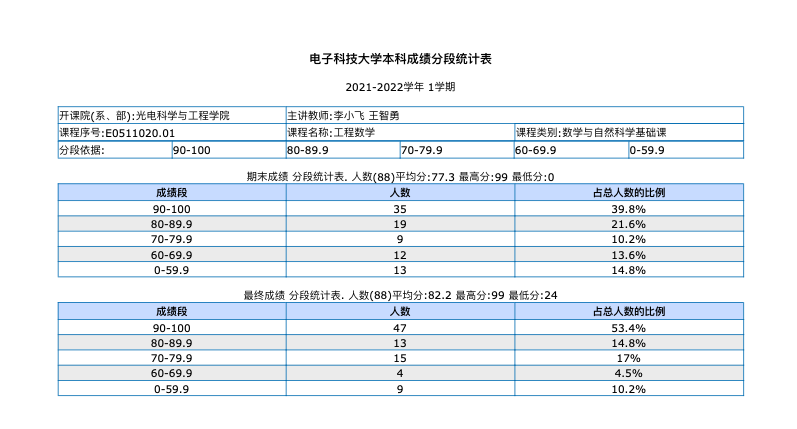
\includegraphics[width=1.0\textwidth,height=5.0cm]{figs/exam1.png}
\end{frame}

\begin{frame}
    \frametitle{参考书目}
        \begin{itemize}
            \Item 《量子力学》卷I,II, 曾谨言, 科学出版社, 2008           
            \Item Principles of quantum mechanics, shankar
            \Item Modern quantum mechanics, shankar
            \Item Lectures on quantum mechanics, weinberg
            \Item Principles of quantum mechanics, Dirac
        \end{itemize}
\end{frame}

\begin{frame}
    \begin{tcolorbox4}[三条军规]    
        \begin{enumerate}
            \Item Objects are wave-particles and can be in states of superposition
            \Item Rule 1 holds as long as you don't measure
            \Item Measurement gives random results
        \end{enumerate}
    \end{tcolorbox4} 
\end{frame}

\section{2.能量子假说}

\subsection{伟大成就}

\begin{frame}[t]
    \frametitle{经典物理伟大成就}
    \begin{tcolorbox3}
    [Great successes in Classical Physics]
        \begin{enumerate}
            \Item Newtonian mechanics
            \Item Maxwell's electromagnetism
            \Item Thermodynamic laws
        \end{enumerate}
    \end{tcolorbox3}  
    \begin{quotation}
        "There is nothing new to be discovered in physics now. All that remains is 
        more and more precise measurements"   \\
        \rightline{$\cdots$ Lord Kelvin (1900)\hspace{3em}}
    \end{quotation}
\end{frame}

\begin{frame}
    \frametitle{}
    \begin{quotation}
        "But the beauty and clearness ... is obscured by two small puzzling clouds \faCloud "  \\
        \rightline{$\cdots$ Lord Kelvin (1900.4)\hspace{3em}}   
    \end{quotation}
    ~~ \vspace{0.3em}
    \begin{tcolorbox4}[两朵乌云]    
        \begin{enumerate}
        \Item Michelson-Morley experiment
        \Item Black body radiation
        \end{enumerate}
    \end{tcolorbox4} 
\end{frame}

\begin{frame}
    \frametitle{迈克尔逊-莫雷实验}
    \begin{center}
    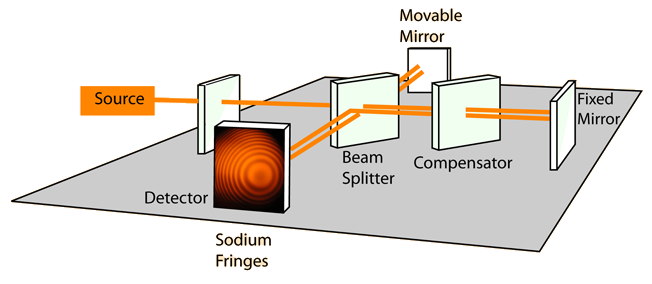
\includegraphics[width=0.8\textwidth]{figs/michel.png}
    \end{center}
There is no displacement of the interference bands. \dots 
the Stationary Ether is thus shown to be incorrect
\end{frame}

\begin{frame}
    The theory of relativity is established 
    \begin{center}
        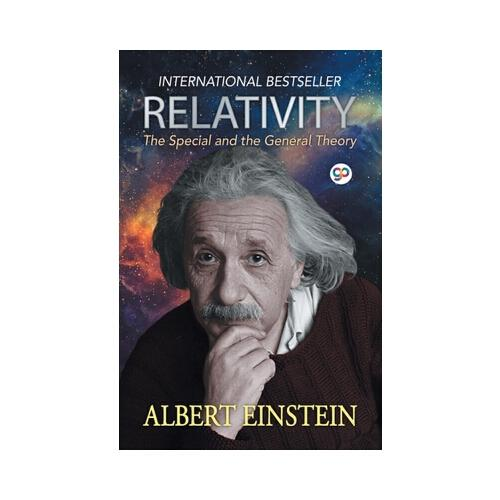
\includegraphics[width=0.4\textwidth]{figs/relativity.jpg}
    \end{center}   
    Greatly changed our view of time and space. Mainly useful in two aspects: high-speed motion, and strong gravitational field. 
\end{frame}

\begin{frame}
    \frametitle{黑体辐射实验}
    \begin{center}
    \includegraphics[width=0.7\textwidth]{figs/2021-12-01-23-47-27.png}
    \end{center}
    No mathematical function to describe the curves exactly 
\end{frame}
\begin{frame}
    Quantum mechanics is established  
    \begin{center}
        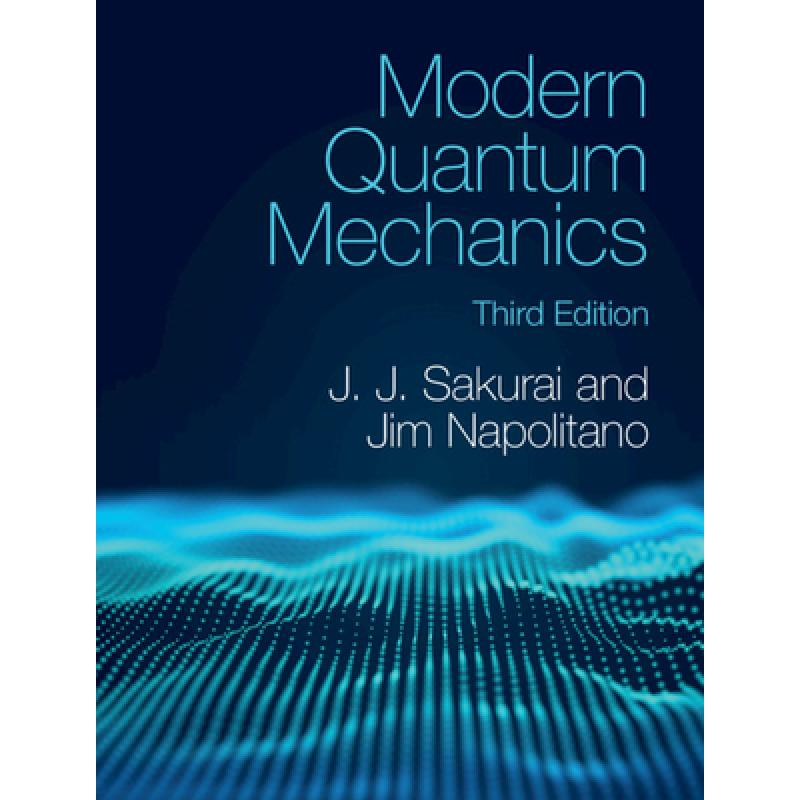
\includegraphics[width=0.45\textwidth]{figs/mqm.jpg}
    \end{center}   
    It is a theory about matter.
\end{frame}

\begin{frame}
    \frametitle{现代科学基石}
    \begin{center}
        \includegraphics[width=0.75\textwidth]{figs/stone.png}
    \end{center}   
\end{frame}

%%%%%%%%%%%%%%%%%%%%%%%%%%%%%%%%%%%%
\subsection{普朗克公式}
%%%%%%%%%%%%%%%%%%%%%%%%%%%%%%%%%%%%

\begin{frame}
    \frametitle{Black body radiation}
    \begin{definition}[Black body: ]
    \hspace{2em}absorb all electromagnetic waves in any temperature
    \end{definition}
    \begin{center}
        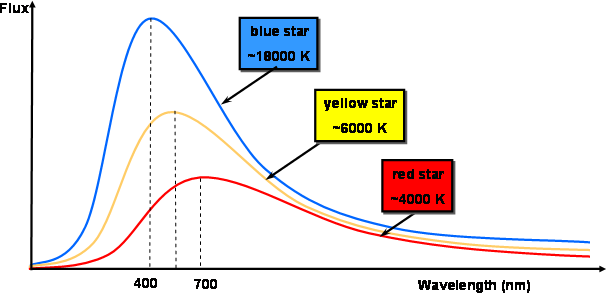
\includegraphics[width=0.55\textwidth]{figs/blackbody_radn_curves.png}
    \end{center}
    \textbf{\color{deepred} Most interestingly}, what is the mathematical function that describes all of these curves?
\end{frame}

\begin{frame}
    \frametitle{三个经验公式}
    \begin{center}
        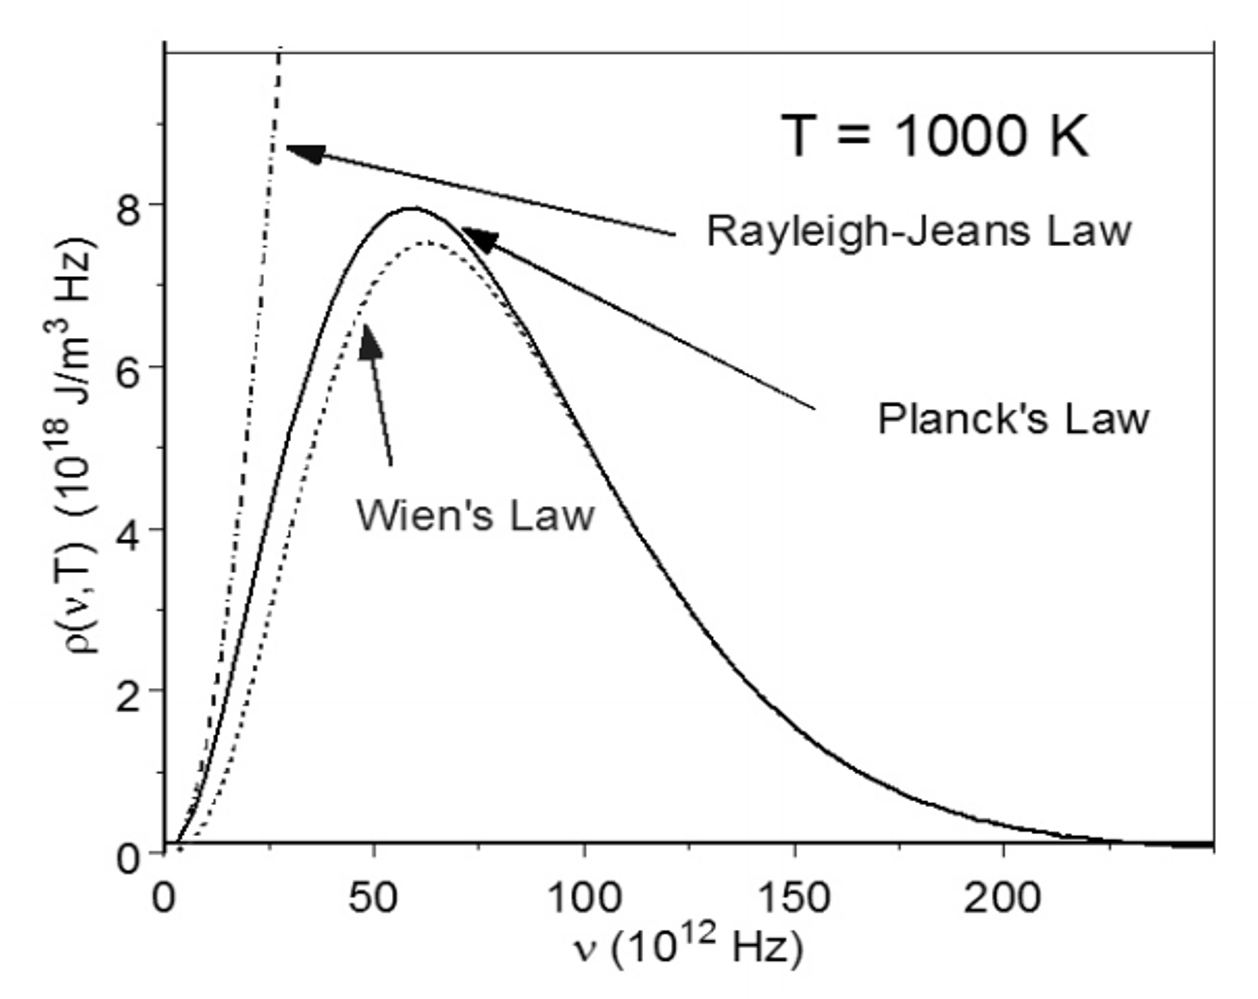
\includegraphics[width=0.7\textwidth]{figs/threelaws.png}
    \end{center}
\end{frame}

\begin{frame} [t]
    \frametitle{维恩公式}
    \begin{equation*}
        \rho(\nu) d \nu=c_{1} \nu^{3} e^{-c_{2} \nu / T} d \nu 
    \end{equation*}
    Derived from electromagnetism (1893), but described well only in high frequency region.\\ 
    {\color{deepred} Nobel Prize in physics(1911)}\\
\end{frame}

\begin{frame}[t]
    \frametitle{瑞-金公式}
    \begin{equation*}
        \rho(\nu, T) d \nu=\frac{8 \pi}{c^{3}} \nu^{2} k T d \nu 
    \end{equation*}
    Derived from thermodynamics (1900), but described well only in low frequency region.\\ 
   {\color{deepred} Nobel Prize in physics(1904)}\\ \vspace{0.3em}
   {\color{deepblue} {\Bullet} Ultraviolet Catastrophe:} 
    \begin{equation*}
         \int_0 ^\infty \frac{8 \pi}{c^{3}} \nu^{2} k T d \nu \to \infty 
    \end{equation*}
\end{frame}

\begin{frame}
    \frametitle{普朗克公式}
    On 1900-10-19, at the German Physical Society, 
    Max Planck presented a resolution to {\color{deepblue} Ultraviolet Catastrophe} 
    \begin{equation}
        \boxed{\rho(\nu, T) d \nu=\frac{8 \pi}{c^{3}} \frac{h \nu^{3}}{e^{h \nu / K T}-1} d \nu}
    \end{equation}
    Obtained from experimental data via interpolation technique, described well in whole region \\
    {\color{deepred} Nobel Prize in physics(1918)}\\
\end{frame}

\begin{frame}
    \centering
    \begin{tcbb}[0.7]{Problems}{
        How to derive the formula from existing theory.}
    \end{tcbb}
\end{frame}

\begin{frame}
    \begin{tcolorbox2}{Solution}
        On 1900-12-14, Planck gives out his solution based on the Energy Quantum Hypothesis  
    \end{tcolorbox2}
\end{frame}

%%%%%%%%%%%%%%%%%%%%%%%%%%%%%%%%%%%%
\subsection{能量子假说}
%%%%%%%%%%%%%%%%%%%%%%%%%%%%%%%%%%%%
\begin{frame}{能量子假说}
    \begin{tcolorbox4}[Energy quantum hypothesis]
    Assuming the oscillators of the cavity could only radiate at a discrete amounts of energy
    \begin{equation}
        E=n\varepsilon
    \end{equation}
    where, the $\varepsilon$ is the unit of the energy (quanta) determined by the oscillator' frequency 
    \begin{equation}
        \varepsilon=h\nu
    \end{equation}
    and the $h=6.6260693(11)\times10^{-34} J\cdot s,\quad (\hbar=\frac{h}{2\pi} \approx 6.58\times 10^{-16} eV\cdot s )$ is the Planck constant. 
    \end{tcolorbox4}
\end{frame}

\begin{frame} {推导公式}
    Based on Boltzmann distribution law,
    \begin{equation*}
        \frac{N_{i}}{N}=\frac{\exp \left(-\frac{E_{i}}{k T}\right)}{\sum_{i} \exp \left(\frac{-E_{i}}{k T}\right)}
    \end{equation*}
    {\Bullet} when the energy is continuous,the distribution between $E - dE$ should be 
    \begin{equation*}
        \frac{e^{-E / k T}}{\int\limits_{0}^{\infty} e^{-E / k T} d E}
    \end{equation*}  
    the average energy 
    \begin{equation*}
        <E>=\int\limits_{0}^{\infty} E \frac{e^{-E / k T}}{\int\limits_{0}^{\infty} e^{-E / k T} d E} d E
    \end{equation*}
\end{frame}

\begin{frame}
    \begin{equation*}
        \begin{split}
            <E> &= -kT \frac{Ee^{-E / k T}\vert_0 ^\infty-\int\limits_{0}^{\infty} e^{-E / k T} d E } {\int\limits_{0}^{\infty} e^{-E / k T} d E }\\  
                &= kT
        \end{split}  
    \end{equation*} 
    {\Bullet} when the energy is discrete,the distribution should be   
    \begin{equation*}
        \frac{e^{-E / k T}}{\int\limits_{0}^{\infty} e^{-E / k T} d E} 
        \to \frac{e^{-E / k T}}{\sum\limits_{0}^{\infty} e^{-E / k T}} 
        \to \frac{e^{-nh\nu / k T}}{\sum\limits_{0}^{\infty} e^{-nhv / k T}} 
    \end{equation*}    
\end{frame}

\begin{frame}
    the average energy 
    \begin{equation*}
        \begin{split}
            <E> &= \sum\limits_{0}^{\infty} nh\nu\frac{e^{-nh\nu / k T}}{\sum\limits_{0}^{\infty} e^{-nh\nu / k T}} \\
            &= -h\nu \frac{d}{dx} \frac{n e^{-nx}}{\sum\limits_{0}^{\infty} e^{-nx}} \\
            &= \frac{h\nu}{e^{h\nu/kT}-1} 
        \end{split} 
    \end{equation*}
    We get
    \begin{equation*}
        \text{(continuous)} \quad k T \rightarrow \frac{h \nu}{e^{ h \nu / k T}-1} \quad \text{(discrete)} 
    \end{equation*}
\end{frame}

\begin{frame}
    In Rayleigh-Jeans formula
    \begin{equation*}
        \rho(\nu, T) d \nu=\frac{8 \pi}{c^{3}} \nu^{2} k T d \nu 
    \end{equation*}
    the item $kT$ should be replaced by $\dfrac{h \nu}{e^{ h \nu / k T}-1}$
    \begin{equation*}
        \rho(\nu, T) d \nu=\frac{8 \pi}{c^{3}} \frac{h \nu^{3}}{e^{h \nu / K T}-1} d \nu
    \end{equation*}
    It is the Planck's formula exactly 
\end{frame}

\begin{frame}
    \begin{tcolorbox4}[Revolutionary Significance]
        Planck's Energy Quantum Hypothesis broke through the constraints of classical physics and 
        opened the door of quantum mechanics 
    \end{tcolorbox4}
\end{frame}

\begin{frame}
    \frametitle{}
    \centering
    \tcbb[0.68]{一只会下金蛋的鹅}
    {
    历史上,普朗克,德拜,艾伦菲斯特,劳厄,洛伦兹,庞加莱,泡利,玻色,爱因斯坦等从多角度推导过普朗克公式,每一次推导都给物理学带来了新的知识内容 
    }

 《黑体辐射公式的多种推导及其在近代物理构建中的意义》- 返朴|曹则贤
\end{frame}

%\begin{frame}
%    \begin{tcolorbox}[colback=yellow!10,colframe=red!75!black,title=THE END]
%    In 1927, Dirac got the Planck's formula from Quantum Mechanism.  
%    \end{tcolorbox}
%\end{frame}

\begin{frame}
    \frametitle{}
    \begin{tcolorbox3}[学术讨论]
        普朗克黑体辐射公式重要,还是能量量子化观念重要?\\
        能量量子化只是一种数学处理工具?
    \end{tcolorbox3}
\end{frame}

%%%%%%%%%%%%%%%%%%%%%%%%%%%%%%%%%%%%%%%%%%%%%%%%%%%%%%%%%%%%%%%%%%%
\begin{frame}
    \frametitle{作业}
   \begin{enumerate}
       \item Planck's Energy Quantum Hypothesis
       \item What's the quanta
       \item Deriving the Rayleigh-Jeans formula and Wien's formula from Planck's formula
   \end{enumerate}
\end{frame}
%%%%%%%%%%%%%%%%%%%%%%%%%%%%%%%%%%%%%%%%%%%%%%%%%%%%%%%%%%%%%%%%%%%

\section{3.波粒二象性}      

\begin{frame}
    \frametitle{}
    \begin{tcolorbox3}[前情回顾]
        Assuming the oscillators can radiate at a discrete amounts of energy
        \[    E=n\varepsilon, \qquad (n=1,2,3,\cdots) \]
        and the unit of the energy is determined by the oscillator' frequency
        \[   \varepsilon=h\nu  \]
        one can derive the framula:
        \[ \rho(\nu, T) d \nu=\frac{8 \pi}{c^{3}} \frac{h \nu^{3} }{e^{h \nu / K T}-1} d \nu \]
    \end{tcolorbox3}
\end{frame}

\begin{frame}
    \frametitle{粒-波的不可调和性}
	\begin{columns}
		\begin{column}[t]{0.46\linewidth}
			粒子性
			\begin{itemize}
				\Item  确定的位置、能量、动量等
				\Item  两个粒子不能同时占据同一位置
				\Item  同一粒子也不能同时占据多个位置
				\Item  碰撞现象
			\end{itemize}
		\end{column}
		\begin{column}[t]{0.46\linewidth}
			波动性
			\vspace{1ex}
			\begin{itemize}
				\Item  确定的波长、振幅、相位等
				\Item  可以同时出现在同一位置
				\Item  可以同时占据多个位置
				\Item  衍射、干涉,无碰撞
			\end{itemize}
		\end{column}
	\end{columns}
\end{frame}

\begin{frame} 
    人们通过上述特性进行判定\\
    \begin{itemize}
        \Item  一个物体要么是粒子,要么是波
        \Item  这个方法一直是有效
        \Item  直到遇到**光** 
    \end{itemize}   
    \begin{figure}
        \centering
        \subfigure[]{\includegraphics[width=7.4cm]{figs/2021-12-02-15-26-40.png}}
        \subfigure[]{
\includegraphics[width=4.5cm]{figs/2021-12-06-11-44-50.png}}
        %\caption{} %图片标题
        %\label{fig:1}  
    \end{figure} 
    \setcounter{subfigure}{0}
\end{frame}

\begin{frame}
	\begin{columns}
		\begin{column}[t]{0.46\linewidth}
            水波
            \begin{center}
                \includegraphics[width=2.5in,height=2.5in]{figs/2021-12-02-15-46-16.png}
            \end{center}
		\end{column}
		\begin{column}[t]{0.46\linewidth}
            光波
            \begin{center}
                \includegraphics[width=2.5in,height=2.5in]{figs/2021-12-02-15-49-36.png}
            \end{center}
		\end{column}
	\end{columns}
\end{frame}

\begin{frame} {光的波动说}
    \begin{center}
        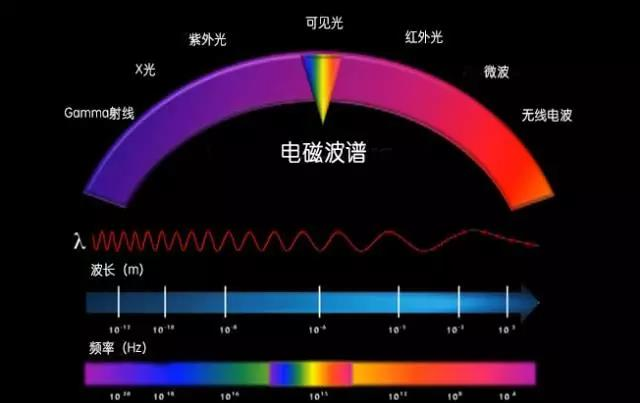
\includegraphics[width=0.70\textwidth]{figs/2021-12-02-16-23-16.png}
    \end{center}
    光只是一定波长范围内的电磁波
\end{frame}

\begin{frame} 
    波动说面临的困难:
    \begin{itemize}
        \Item  黑体辐射
        \Item  光电效应
        \Item  康普顿效应
        \Item  氢原子光谱
    \end{itemize}
\end{frame}

%%%%%%%%%%%%%%%%%%%%%%%%%%%%%%%%%%%%
\subsection{光电效应}
%%%%%%%%%%%%%%%%%%%%%%%%%%%%%%%%%%%%

\begin{frame} 
    \frametitle{光电效应实验}   
    \begin{center}
       \includegraphics[width=0.53\textwidth]{figs/2021-12-02-16-01-21.png}
   \end{center}  
   {\Bullet} 具有瞬时性 \\
   {\Bullet} 存在临界频率 $\nu_0$ \\
   {\Bullet} 光电子能量由光的频率决定
\end{frame}  

\begin{frame} 
    In 1905, Einstein considered the derivation of Planck's Law  \\
    \begin{itemize}
        \Item  Plank’s Law was consistent with experment but not with existing theory
        \Item  Rayleigh-Jeans Law was consistent with existing theory but not with experiment
        \Item  For treating Ultraviolet Catastrophe, he proposed the light quantum hypothesis
        \Item  Using light quantum hypothesis, he explained the Photoelectric effect
    \end{itemize}
\end{frame}

\begin{frame}
    \frametitle{}
        \begin{figure}
            \centering
            \subfigure[光强分布]{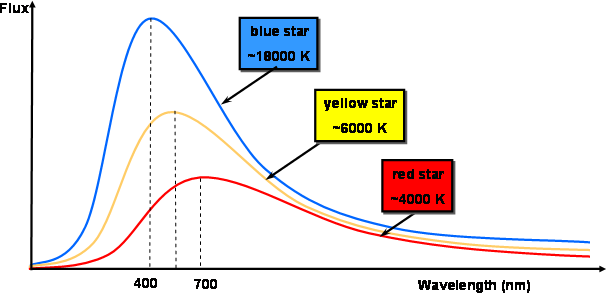
\includegraphics[width=0.495\textwidth]{figs/blackbody_radn_curves.png}}
            \subfigure[粒子数分布]{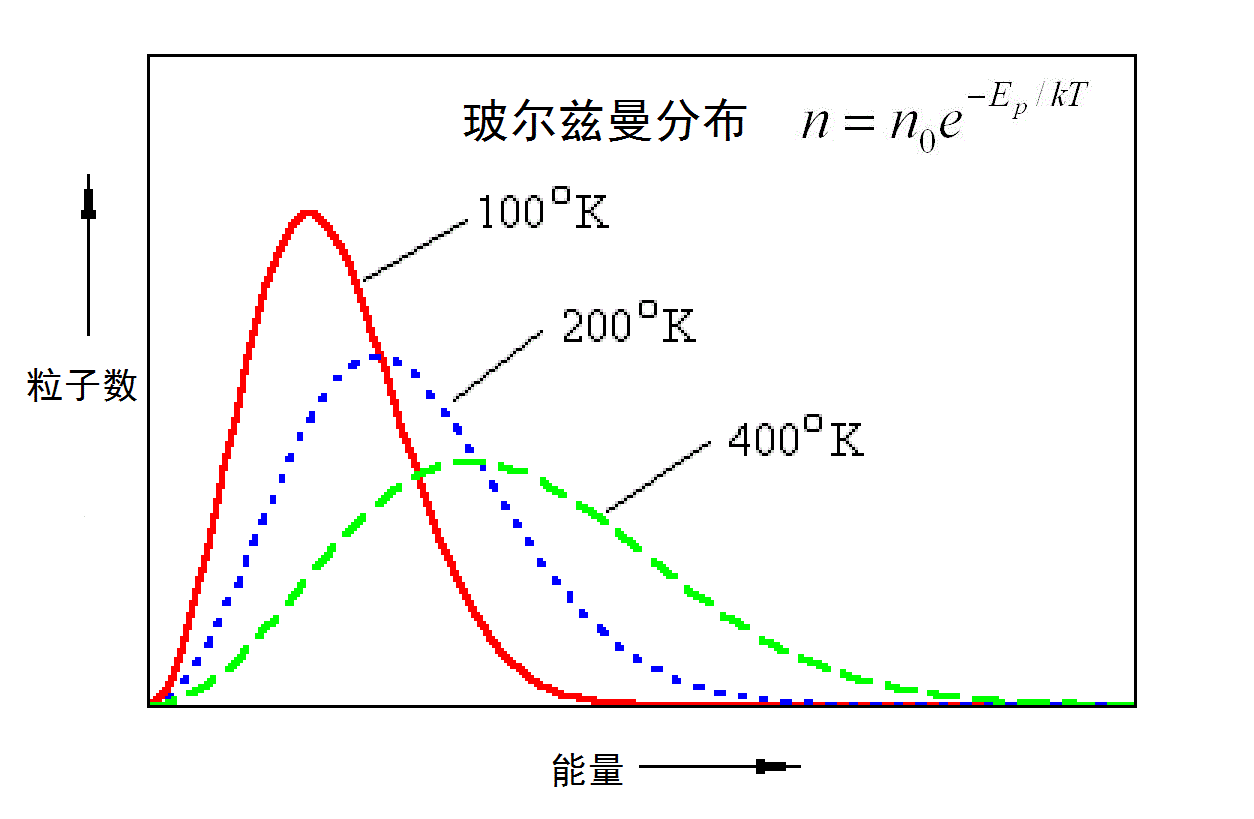
\includegraphics[width=0.495\textwidth]{figs/2022-01-17-14-21-43.png}}
        \end{figure}
    \setcounter{subfigure}{0}
\end{frame}

\begin{frame} 
    \begin{tcolorbox4}[Light quantum hypothesis]
        {\Bullet} Light likes particles with unit energy  (quanta).\\
        \[E=h\nu\]  
        {\Bullet} The energy of n light quantum is $nh\nu$. \\
        {\Bullet} The momentum of light quantum is (1918) \\
        \[p=\frac{E}{c}=\frac{h\nu}{c}=\frac{h}{\lambda}\]
    \end{tcolorbox4}
\end{frame}

\begin{frame} 
    基于光量子假说,提出光电效应公式
    \[
    \frac{1}{2}m_eV_0^2=h\nu-W
    \]
    \begin{itemize}
        \Item  瞬时性:光如果是粒子,碰上电子则能量被瞬时吸收
        \Item  临界频率:$\nu_0=\frac{W}{h} $
        \Item  光电子能量与光的频率决定: $E_k=h\nu-W$
    \end{itemize}
    {\color{deepred} Nobel Prize in physics(1921)}
\end{frame}

\begin{frame} 
    基于光电效应公式:
$$
\frac{1}{2}m_eV_0^2=h\nu-W
$$
1916年,密立根实验上测定普朗克系数,验证光子说\\
\color{deepred}{1923年诺贝尔物理学奖} 
\end{frame}

\begin{frame} 
    \begin{tcolorbox4}[光量子假说的意义]
        \begin{itemize}
            \Item  揭示能量子的本质:在于光本身是量子化的,具有粒子性
            \Item  揭示光的本质:光既具波动性又具粒子性。
        \end{itemize}
    \end{tcolorbox4}
    \begin{quotation}
        "在近代物理学结出硕果的那些重大问题中,很难找到一个问题是爱因斯坦没有做出过重要贡献的。
        在他的各种推测中,他有时可能也曾经没有中标的,例如他的光量子假设,就有点迷失了方向\dots"  \\
        \rightline{$\cdots$ 普朗克\hspace{3em}}   
    \end{quotation}
\end{frame}

%%%%%%%%%%%%%%%%%%%%%%%%%%%
\subsection{康普顿效应}
%%%%%%%%%%%%%%%%%%%%%%%%%%%

\begin{frame}   
    \frametitle{康普顿效应 (1922)}
    \begin{center}
        \includegraphics[width=0.7\textwidth, height=3in]{figs/comptonscattering.png}
    \end{center}  
\end{frame}

\begin{frame} 
    ~~\\ 
    经验公式:$\lambda_{out}-\lambda_{in}=\lambda_e(1-\cos \theta)$ \\  \vspace*{0.6em}
    \alert{解:} Energy of electron 
    \begin{equation*}
        E^2 =m_ec^2=p^2c^2 +m_0 ^2 c^4 
    \end{equation*}
    Energy of light quantum
    \begin{equation*}
        E =pc 
    \end{equation*}
    energy conservation law
    \begin{equation*}
        \begin{split}
        E_i + m_0 c^2 &= E_o + m_ec^2 \\
        (E_i -E_o + m_0 c^2)^2 &= E_e ^2\\
        (p_i c-p_o c + m_0 c^2) ^2 &= p_e ^2 c^2 +m_0 ^2 c^4 \\
        (p_i-p_o)^2 +2 m_0 (p_i c-p_o c) &= p_e ^2
    \end{split}
    \end{equation*}
\end{frame}

\begin{frame}  
    momentum conservation law
    \begin{equation*}
        \begin{split}
            \vec{p}_i -\vec{p}_o &= \vec{p}_e \\
            (\vec{p}_i -\vec{p}_o)\cdot (\vec{p}_i -\vec{p}_o)  &= \vec{p}_e\cdot \vec{p}_e   \\
            p_i ^2 + p_o ^2 -2p_i p_o \cos \theta &= p_e ^2  \\
            p_i ^2 + p_o ^2 -2p_i p_o \cos \theta &= (p_i-p_o)^2 +2 m_0 (p_i c-p_o c) \\
            \frac{1}{p_o} -\frac{1}{p_i} &= \frac{1}{m_0 c} (1-\cos \theta) \\
            \lambda_o -\lambda_i &= \frac{h}{m_0 c} (1-\cos \theta) 
        \end{split}
    \end{equation*}
\end{frame}

\begin{frame}   
    \begin{tcolorbox3}[Significance]
        Prove that:\\
        {\Bullet} The light of wavelength ($\lambda$) possesses a quantum momentum \[p=\frac{h}{\lambda}\]
        {\Bullet} Momentum conservation law works in subatom scales 
    \end{tcolorbox3}   
    \color{deepred}{Nobel Prize in physics(1927)}\\
\end{frame}

%%%%%%%%%%%%%%%%%%%%%%%%%%
\subsection{氢原子光谱}
%%%%%%%%%%%%%%%%%%%%%%%%%%

\begin{frame}  
     \frametitle{氢原子光谱}
     \begin{center}
        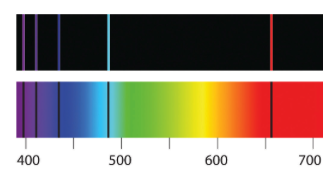
\includegraphics[width=0.6\textwidth]{figs/2022-01-17-14-02-45.png}
    \end{center}  
    经验公式:
       $\dfrac{1}{\lambda}=R_H c (\dfrac{1}{m^2} -\dfrac{1}{n^2})$ \\ \vspace{0.3em}
    \alert{Problem:} the formula cannot be derived from existing theory
\end{frame}

\begin{frame} 
    \frametitle{Rutherford model}  
    \begin{center}
        \includegraphics[width=0.8\textwidth]{figs/utherford_atom.png}
    \end{center}  
\end{frame}

\begin{frame}  
    \begin{tcolorbox4}[Bohr's hydrogen atom hypothesis]
    Bohr asummed that :\\
    {\Bullet} Stationary states: Electrons move around the nucleus only in certain allowed circular orbits with fixed energy \\
    \[ L=n \frac{h}{2\pi}= n \hbar,\qquad (\oint p_i dq_i = n_i h)\]
    {\Bullet} Quantum transition: Electron can jump between stationary state orbits when absorbed or emitted a photon with certain energy\\
    \[ h\nu=E_n -E_m \]
    \end{tcolorbox4}
\end{frame}

\begin{frame}   
    \frametitle{}
    推导光谱公式\\
    {\Bullet} Stationary state orbit radius:
    \begin{equation*}
        \begin{split}
            m\frac{v^2}{r}&=\frac{1}{4\pi\epsilon_0} \frac{e^2}{r^2} \\
            L=&mvr =n\hbar \\
            r_n&= n^2 (\frac{\epsilon_0 h^2}{m\pi e^2}) =n^2 r_1   
        \end{split} 
     \end{equation*}
     {\Bullet} Stationary state orbit energy: 
     \begin{equation*}
        \begin{split}
            E_n &= T + U \\
            &= \frac{1}{2}mv^2- \frac{1}{4\pi\epsilon_0} \frac{e^2}{r_n ^2} \\
            &= \frac{1}{n^2} (-\frac{m e^4}{8 \epsilon_0 ^2 h^2}) = \frac{E_1}{n^2}
        \end{split}  
     \end{equation*}
\end{frame}

\begin{frame}
    {\Bullet} Spectrum formula: 
    \begin{equation*}
        \begin{split}
         \nu&=\frac{E_n -E_m}{h} \\
         &= \frac{m e^4}{4\pi \hbar ^3} [\frac{1}{m^2} -\frac{1}{n^2}]
        \end{split}  
     \end{equation*}
     {\Bullet} Rydberg constant : 
     \[R_{theo}= \frac{m e^4}{4\pi \hbar ^3 c} =1.0973731\times 10^7 m^{-1}\]
    \[R_{exp}=1.0974\times10^7 m^{-1} \]  
\end{frame}

\begin{frame}   
    \frametitle{Bohr's model}  
    \begin{center}
        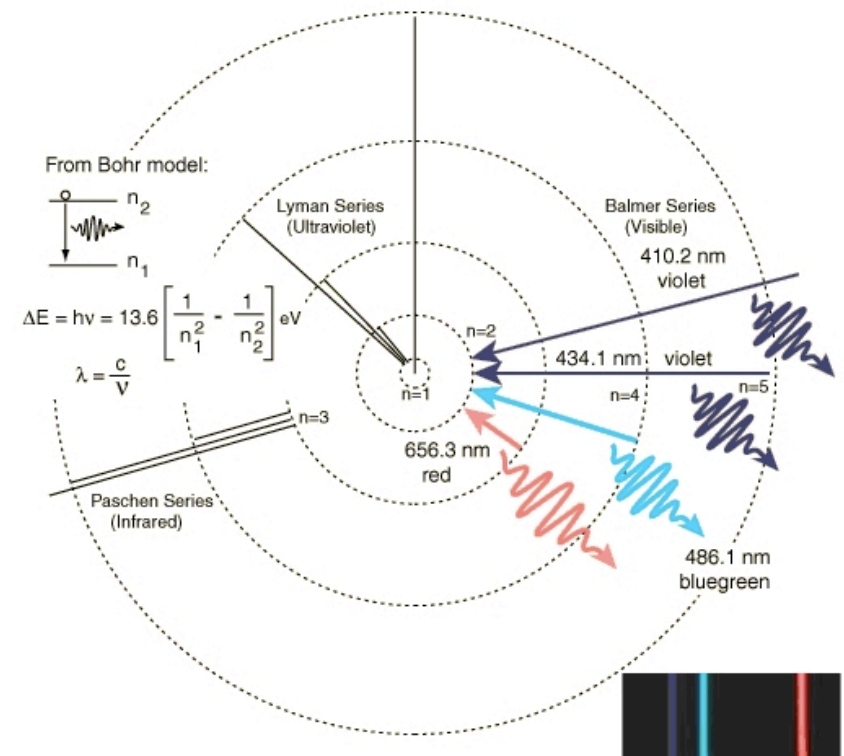
\includegraphics[width=0.6\textwidth]{figs/bohrmodel.png}
    \end{center}  
    {\Bullet} 1905年爱因斯坦提出的光子概念,不受名人的重视,普朗克把爱因斯坦的光量子概念说成是“迷失了方向”。\\
    {\Bullet} 1913年,28岁的玻尔,创造性地把光子概念用到卢瑟福模型上,成功破解氢原子光谱问题 \\
    {\color{deepred} {\Bullet} Nobel Prize in physics(1922)}\\ 
\end{frame}

\subsection{光的波粒二象性} 

\begin{frame} 
  \frametitle{光的波粒二象性}  
  {\Bullet} In 1905, when Einstein first put forward this hypothesis, 
  he simply stated that light consisted of quanta with energy \[ E = h\nu \] 
  {\Bullet} In 1917, he stated that the light quantum carried a momentum of  \[ p=\frac{h}{\lambda}\]
  At this point, the light quantum with massless particle property was named as photon (光子)
\end{frame}

\begin{frame}  
  $\begin{cases}
    \text{Light behaves like waves }\\
    \text{~~\qquad Interference} \\
    \text{~~\qquad Diffraction} \\
    \text{Light behaves like particles}\\
    \text{~~\qquad Black body radiation} \\
    \text{~~\qquad Photoelectric effect} \\
    \text{~~\qquad Compton effect} \\
   \end{cases}$\\
   ~~\\
   Light has both wave and particle properties is called \alert{wave-particle duality} of light
\end{frame}

\begin{frame}
    \frametitle{}
    \begin{tcolorbox3}[学术讨论]
        ~\\
        How can the light be both particle and wave ?
    \end{tcolorbox3}
\end{frame}

%%%%%%%%%%%%%%%%%%%%%%%%%%%
\subsection{物质波假说}
%%%%%%%%%%%%%%%%%%%%%%%%%%%

\begin{frame}   
  \frametitle{物质波假说}
  \begin{tcolorbox4}[Matter wave hypothesis]
  In 1923, de Broglie states that if light which is classically a wave could behave as a particle
  then classical particles could also behave as quantum waves. The wave length and frequency are
  \[\lambda=\frac{h}{p}\]
  \[\nu =\frac{E}{h}\]
  \end{tcolorbox4}
\end{frame}

\begin{frame}  
    \frame{}
    Calculating de Broglie wavelength of electron in Bohr's H atom model
    \begin{equation*}
        \begin{split}
            L&=n\hbar \\
            \vec{r} \cdot \vec{p} & =  n\frac{h}{2 \pi} \\
            2\pi r&=  n\frac{h}{p}\\
            2\pi r&=  n\lambda 
        \end{split} 
     \end{equation*}
     Now, we called it standing-wave condition 
\end{frame}


\begin{frame}   
  \frametitle{Experimental verification}
  \begin{center}
    \includegraphics[width=0.5\textwidth]{figs/elediffr.jpeg} \\
    Electron diffraction patterns (Davisson and Germer, 1927)
    \end{center} 
\end{frame}
\begin{frame}   
    \begin{center}
      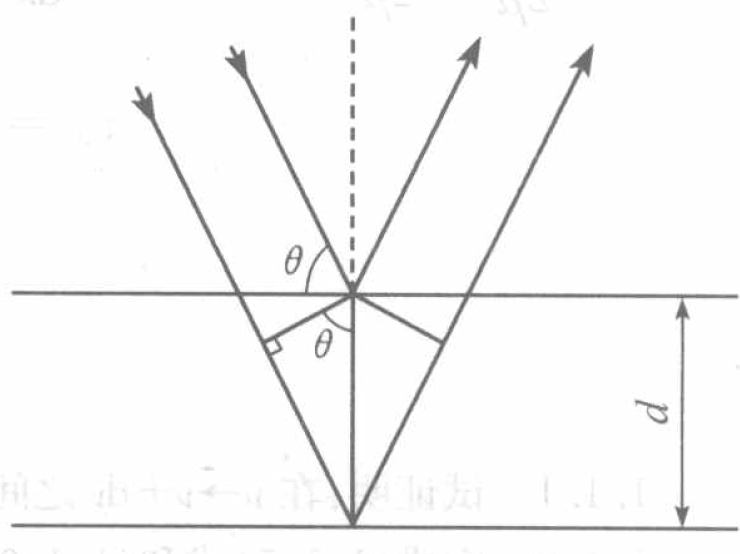
\includegraphics[width=0.55\textwidth]{figs/scatting.png} \\
    \end{center} 
    \begin{itemize}
        \Item  Meeting Bragg formula $2d\sin \theta=n\lambda $
        \Item  Obtaining the wavelength of electron (about 0.16X $nm$), agreeing well with the 
   calculated de Broglie wavelength 
    \end{itemize}
  {\color{deepred} Nobel Prize in physics(1937)}  
  \end{frame}

  \begin{frame}
      \frametitle{}
    \begin{center}
         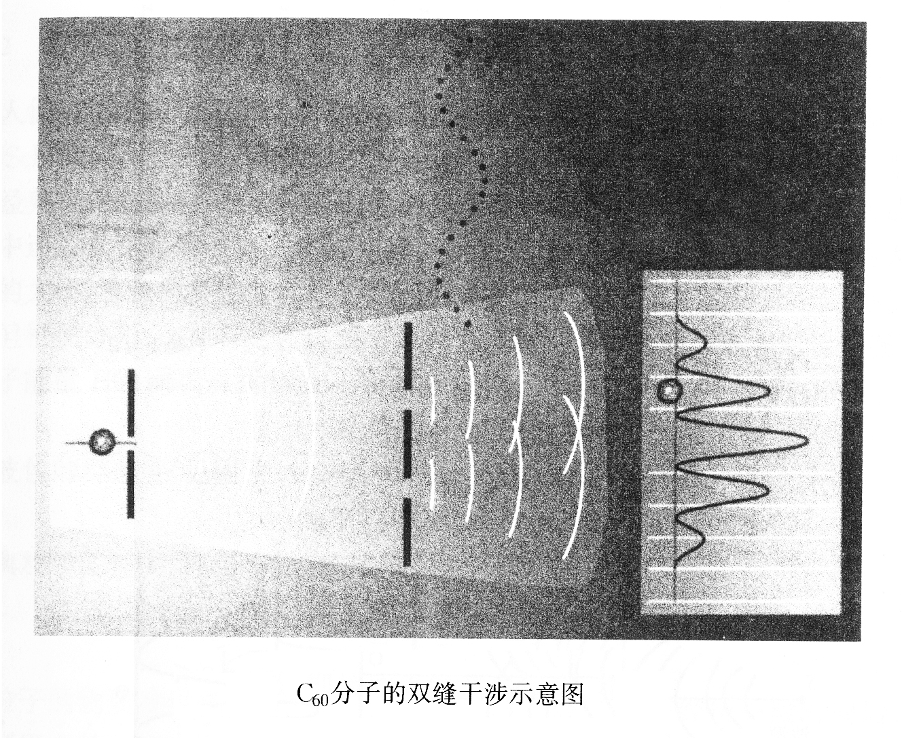
\includegraphics[width=0.8\textwidth,height=2.5in]{figs/c60.png}
    \end{center}
  \end{frame}
\begin{frame} 
    \begin{tcolorbox}[colback=yellow!10,colframe=red!75!black,title=Significance]
        De Broglie extended the wave-particle duality from light to particles! \\
        {\color{deepred} Nobel Prize in physics(1929)} for discovery of wave nature of electrons
    \end{tcolorbox}  
\end{frame}

\begin{frame}{电子双缝干涉实验}
    \includemedia[
    width=1.0\linewidth,height=0.67\linewidth, % 16:9
    activate=pageopen,
    addresource=figs/doubleslite-n.mp4,
    flashvars={
    source=figs/doubleslite-n.mp4
    &autoPlay=true % start playing on activation
    &loop=true
    }
    ]{}{VPlayer.swf}
\end{frame}

\begin{frame}
    \frametitle{学术讨论}
        \begin{figure}
            \centering
            \subfigure[]{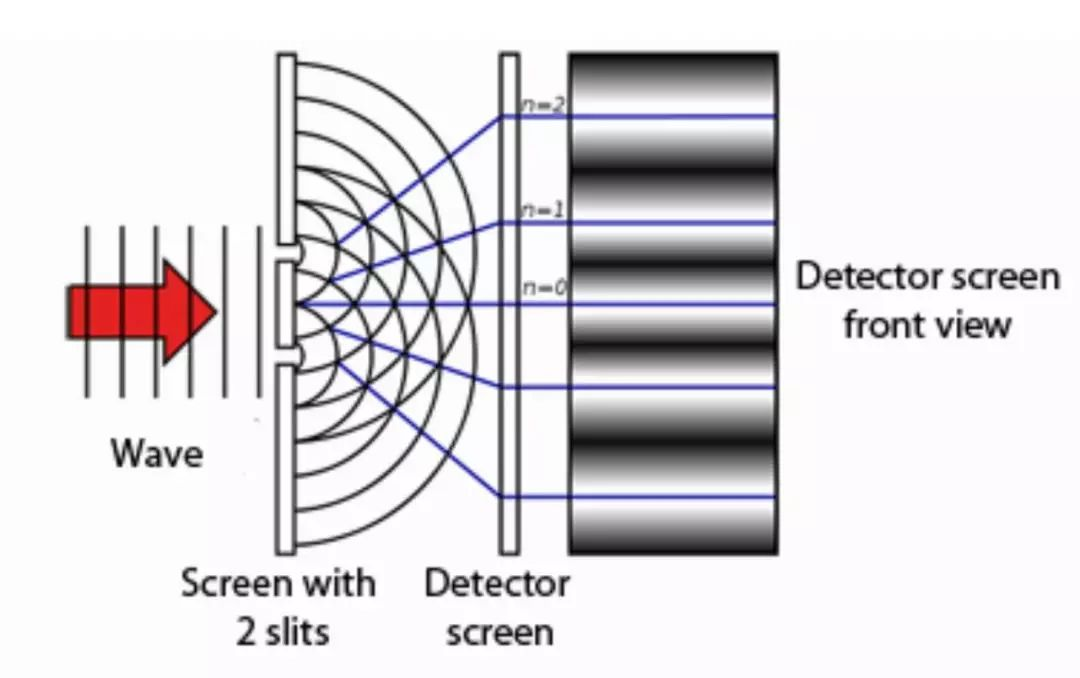
\includegraphics[width=4.5cm]{figs/ds-1.jpeg}}
            \subfigure[]{\includegraphics[width=4.5cm]{figs/ds-2.jpeg}}
            \subfigure[]{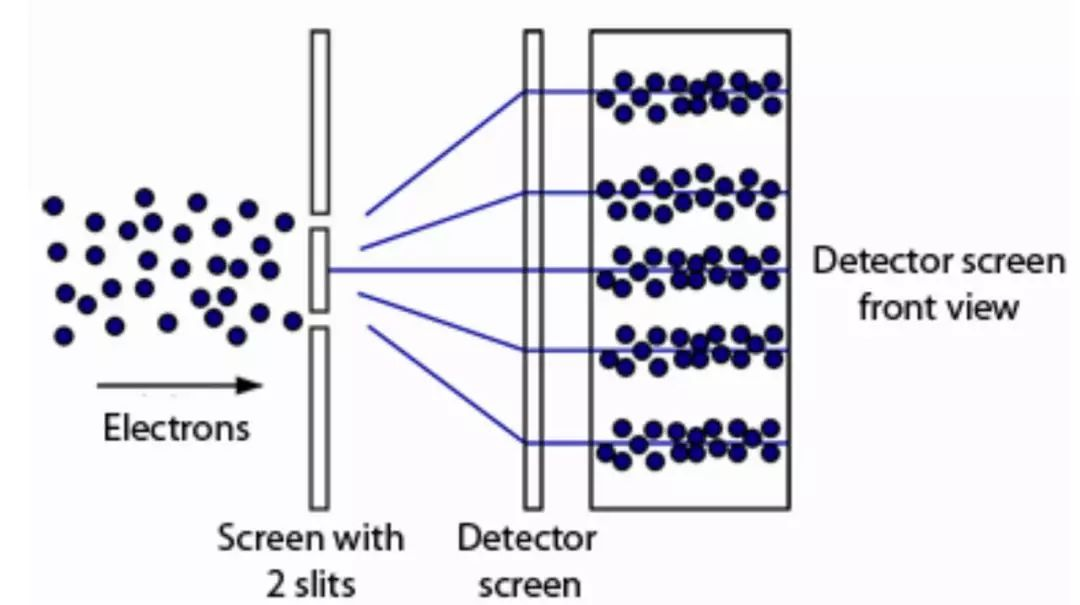
\includegraphics[width=4.5cm]{figs/ds-3.jpeg}}
            %\caption{} %图片标题
            %\label{fig:1}  
            {\color{red} How can electrons be both a particle and a wave?}
        \end{figure}
    \setcounter{subfigure}{0}
\end{frame}

\begin{frame}  
    \begin{tcolorbox3}[Conclusion]
    Wave-particle duality is the inherent attribute of matter
    \end{tcolorbox3} 
\end{frame} 

\begin{frame}
    \frametitle{}
    \centering
    \tcbb[0.5]{Big problems}
    {
      \large  How to interpret a world where waves are particles and particles are waves
    }
\end{frame}

%%%%%%%%%%%%%%%%%%%%%%%%%%%%%%%%%%%%%%%%%%%%%%%%%%%%%%%%%%%%%%%%%%%
\begin{frame}
    \frametitle{课外作业}
    \begin{enumerate}
        \item 计算氢原子第一玻尔半径上电子的德布罗意波长
        \item 计算经 50 V 电势装成加速后电子的德布罗意波长
    \end{enumerate}
\end{frame}
%%%%%%%%%%%%%%%%%%%%%%%%%%%%%%%%%%%%%%%%%%%%%%%%%%%%%%%%%%%%%%%%%%%
%%%%%%%%%%%%%%%%%%%%%%%%%%%%%%%%%%%%%%%%%%%%%%%%%
	\begin{frame}
		\frametitle{}
		\Background[1] 
	    \begin{center}
		{ {\Huge 第二章~~三大偏微分方程\\(6学时)}}
	    \end{center}    
	\end{frame}
%%%%%%%%%%%%%%%%%%%%%%%%%%%%%%%%%%%%%%%%%%%%%

\begin{frame}
	\frametitle{}
	\begin{definition}[] 
	偏微分方程(PDE)指未知函数是多元函数的微分方程,
	方程的函数(物理量)多以时间和空间为变量,这些方程的来源和应用通常具有物理学背景。又称为数学物理方程。
	\end{definition}
	方程的最高阶是二阶的称为二阶偏微分方程
	\begin{equation*}
		au_{xx}+2bu_{xy}+cu_{yy}+du_x+eu_y+fu=g
	\end{equation*}
	根据$\Delta=b^2-ac$二阶偏微分方程可分为三类:椭圆型($\Delta<0$)、双曲型($\Delta>0$)和 抛物型 ($\Delta=0$),\\
	它们的代表分别是:拉普拉斯(泊松方程)、波动方程、热传导方程
\end{frame}

\begin{frame}
\frametitle{三大偏微分方程}
	\begin{itemize}
	\item  波动方程 
	\begin{equation*}
		u_{tt}=a^2u_{xx}
	\end{equation*}
	\item  热传导方程
	\begin{equation*}
		u_t=a^2 \nabla ^2 u 
	\end{equation*}
	\item  拉普拉斯方程
	\begin{equation*}
		 \nabla ^2 u =0
	\end{equation*}
	\end{itemize}
\end{frame}

%%%%%%%%%%%%%%%%%%%%%%%%%%%%%%%%%%%%%%%%%%%%%
\section{1.波动方程}
\subsection{方程的建立}
\begin{frame}
	\frametitle{方程的建立}	
	\begin{exampleblock} {例1、	求弦振动方程}
	考虑均匀柔软的细弦线,二端固定,受到扰动后在平衡位置作微小运动。分析位移函数 u(x,t)满足的方程。\\
	\centering
	\begin{tikzpicture}
	%\draw[eaxis] (0,0) -- (8,0) node[below] {$x$};
	%\draw[eaxis] (0,0) -- (0,0.5) node[right] {$y$};
	\draw (0,0) .. controls (2, 1) and (6,1) .. (8,0);
	\filldraw[red] (0,0) circle [radius=1pt];
	\filldraw[red] (8,0) circle [radius=1pt];
	\end{tikzpicture}
	\end{exampleblock} 	
	自然界普遍存在各种振动,振动的传播形成波,服从统一的方程。	
\end{frame}	

\begin{frame}
	\frametitle{}	
	\begin{center}
		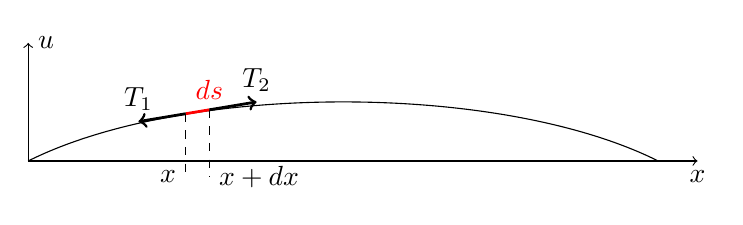
\begin{tikzpicture}
		\draw[->] (0,0) -- (8.5,0) node[below] {$x$};
		\draw[->] (0,0) -- (0,1.5) node[right] {$u$};
		\draw (0,0) .. controls (2, 1) and (6,1) .. (8,0);
		%	\filldraw[red](2,0.6)circle[radius=1pt];
		\draw[dashed] (2,0.6) --(2,-0.2) node[left] {$x$}; 
		%	\filldraw[red](2.3,0.65)circle[radius=1pt];
		\draw[dashed] (2.3,0.65) --(2.3,-0.2) node[right] {$x+dx$}; 
		\draw[red,  line width =1pt] (2,0.6) --(2.3,0.65) node[above] {$ds$};  
		\draw[->, line width =1pt] (2,0.6) --(1.4,0.5) node[above] {$T_1$};  
		\draw[ ->,  line width =1pt] (2.3,0.65) --(2.9,0.75) node[above] {$T_2$};  
	\end{tikzpicture}\\	 \vspace{0.3 em}
	\end{center}
	\alert{解:} 建立坐标系,  取任意微元ds, 临近拉力$T_1, T_2$:\\
	水平:{ $T_2\cos \alpha _2=T_1\cos \alpha _1=T_0$ }  \\   
	竖直:{$T_2\sin \alpha _2-T_1\sin \alpha _1=ma=\rho ds~ u_{tt} $}   \\   
	有~:{ $T_0(\tan \alpha _2-\tan \alpha _1)=\rho ds ~u_{tt}$ }   \\   \vspace{0.3 em}
    \hspace{1cm}$T_0[u_x(x+dx,t)-u_x(x,t)]=\rho dx ~u_{tt}$  \\   \vspace{0.6 em}
	\hspace{1cm}$\displaystyle \frac{T_0}{\rho}\times\frac{u_x(x+dx,t)-u_x(x,t)}{dx}=u_{tt}$ \\ \vspace{0.3 em}
	\Tips (1)斜率就是一阶导,(2)小角度条件下,$ds \simeq dx$
\end{frame}	

\begin{frame}
	\frametitle{}	
	得波动方程:
	\begin{equation*}
		u_{tt}=a^2u_{xx}
	\end{equation*}
	定解条件:\\
	(1) 初始条件 
	$\displaystyle  u(x,t)|_{t=0}= \psi (x) $, 	 $\displaystyle  u_t(x,t)|_{t=0}= \Psi (x) $\\
	(2) 边界条件
	$\displaystyle  u(x,t)|_{x=0}= 0 $, 	 $\displaystyle  u(x,t)|_{x=l}= 0 $\\ 	\vspace{0.3cm} 
	若质点受外力作用, 有:
	\begin{equation*}
		u_{tt}=a^2u_{xx} +f(x,t)
	\end{equation*}
	\begin{block} {Remark}
		波动方程描述了围绕平衡态小幅震荡的规律,它不仅可描述琴弦、鼓膜、耳机的震动,也描述着光波、声波、地震波、引力波,甚至弦论中弦的运动。
	\end{block}
\end{frame}	
%%%%%%%%%%%%%%%%%%%%
\subsection{方程的求解}
\begin{frame}
	\frametitle{方程的求解}	
	\begin{exampleblock} {例2、	求一维波动方程}
	$\displaystyle \begin{cases}
		u_{tt}=a^2u_{xx}\\
		u(x,t)|_{t=0}= \psi (x) ,~~~ u_t(x,t)|_{t=0}= \Psi (x) \\
		u(x,t)|_{x=0}= 0, ~~~  u(x,t)|_{x=l}= 0 
	\end{cases}$ \\	
	\end{exampleblock} %2
	\alert{解:} 	(傅里叶)   设 $\displaystyle  u(x,t)=T(t)X(x) $,代回方程 , 得:
	\begin{equation*}
		 T~^{''}(t)X(x) =a~^2 T(t)X~^{''}(x) 
	\end{equation*}
	 \hspace{1cm} 可分离变量
\end{frame}	

\begin{frame}
	\frametitle{}	
	$ \dfrac{T~^{''}}{a~^2 T}=\dfrac{X~^{''} }{X} =-\lambda $ \\ \vspace{0.3cm}
	转化为两常微分方程 \\ \vspace{0.3cm}
	方程(I):
	$\displaystyle  \begin{cases}
		X~^{''} +\lambda X=0  ~~,~~ 0<x<l\\
		X(0)=0 ~,~X(l)=0
	\end{cases}$ \\	
	方程(II):
	$\displaystyle  \begin{cases}
		T~^{''} +\lambda {a~^2 T}=0 \\
		......
	\end{cases}$ \\	
	\begin{block} {Remark}
		偏微分方程与常微分方程的分离变量法有何不同?
	\end{block}
\end{frame}	

\begin{frame}
	\frametitle{}	
	解方程(I):有特征(辅助)方程, 
	\begin{equation*}
		\mu~^2 +\lambda =0
	\end{equation*}
	根为:
	$\displaystyle  \begin{cases}
		\mu~_1=+\sqrt{-\lambda}\\
		\mu~_2=-\sqrt{-\lambda}
	\end{cases}$ \\	\vspace{0.6 em}	
	{\Bullet}~分情况讨论:\\
	(1) 相异实根($\lambda < 0$)
	有通解:	{ $\displaystyle 	X=Aexp~^{\sqrt{-\lambda}x} + Bexp~^{-\sqrt{-\lambda}x} $ } \\ 
	分别取$x=0, x=l$, 得定解方程组:\\
	$\left[
	\begin{array}{lll}
		1&1\\
		exp~^{\sqrt{-\lambda}~l} &exp~^{-\sqrt{-\lambda}~l}
	\end{array}
	\right]$
	$\left[
	\begin{array}{ll}
		A\\
		B
	\end{array}
	\right]$
	=$\left[
	\begin{array}{ll}
		0\\
		0
	\end{array}
	\right]$
\end{frame}	

\begin{frame}
\frametitle{}	
	有解条件为:
	$\begin{vmatrix}
		1&1\\
		exp~^{\sqrt{-\lambda}~l} &exp~^{-\sqrt{-\lambda}~l}
	\end{vmatrix}
	= 0$\\
	很明显,这个行列式不等于0, 所以只有零解 (A=0,~B=0)    \\ \vspace{0.3cm}
	(2) 相同实根($\lambda = 0$),\\
	则通解为:	{ $\displaystyle 	X=Ax + B $ } \\ 
	分别取$x=0, x=l$, 得定解方程组:\\
	{$\displaystyle \left\{
	\begin{array}{lll}
		B=0\\
		Al+B=0
	\end{array} \right. $}\\
	也只有零解  \\
\end{frame}	

\begin{frame}
	\frametitle{}	
	(3) 虚根($\lambda >0$),即: $ \mu~_1=i\sqrt{\lambda}~~,~~\mu~_2=-i\sqrt{\lambda}$	\\
	通解为:	{ $\displaystyle 	X=A\cos \sqrt{\lambda}x+ B\sin \sqrt{\lambda}x $ } \\ 
	分别取$x=0, x=l$, 得定解方程组:\\
	$\left[
	\begin{array}{lll}
		1&0\\
		\cos( {\sqrt{\lambda}~l}) &\sin ({\sqrt{\lambda}~l})
	\end{array}
	\right]$
	$\left[
	\begin{array}{ll}
		A\\
		B
	\end{array}
	\right]$
	=$\left[
	\begin{array}{ll}
		0\\
		0
	\end{array}
	\right]$\\ 
	系数行列式要为零\\
	$ \sin ({\sqrt{\lambda}~l})=0$ \\
	$ \sqrt{\lambda}~l=n~\pi  (n=1,2,3,...) $\\ 
	\begin{enumerate}
		\IItem 固有值:$\displaystyle  \lambda~_n=\frac{n^2\pi~^2}{l~^2}$ 
		\IItem 固有解:{\large $\displaystyle  X~_n=\sin \frac{n\pi~}{l} x=\sin \omega_n x $}
	\end{enumerate}	
\end{frame}	

\begin{frame}
	\frametitle{}	
	解方程II : 	\[ T~^{''} +\lambda {a~^2 T}=0 \] \\ 
	代入$\lambda_n$, 得:
	$\displaystyle  T~^{''} +\lambda~_n a~^2 ~T=0 $ \\
	变形:$\displaystyle  T~^{''} +\omega ~_n ^2 {a~^2 T}=0 $ \\ 
	特征方程有虚根,通解 :\\
	\hspace{3cm}	$\displaystyle 	T~_n=C~_n\cos \omega_n~a~t+ D~_n\sin \omega ~_n~a~t $  \\ \vspace{1em}
	原方程的基本解:\\
	$\begin{array}{llll}
		u_n(x,t) &=& T_n(t)X_n(x)\\
		&=& (a_n\cos \omega_nat+ b_n\sin \omega _nat ) \sin \omega_n x\\
		&=&(a_n\cos\frac{ n\pi at}{l}+ b_n\sin \frac{ n\pi at}{l}) \sin \frac{ n\pi x}{l}
	\end{array}$ \\ 
\end{frame}	

\begin{frame}
	\frametitle{}	
	叠加解 (解函数):\\
	$\begin{array}{llll}
		u(x,t) &=&\sum\limits_{n=1}^{\infty } u_n(x,t)\\
		&=& \sum\limits_{n=1}^{\infty }  (a_n\cos\frac{ n\pi at}{l}+ b_n\sin \frac{ n\pi at}{l}) \sin \frac{ n\pi x}{l}
	\end{array}$ \\ \vspace{1em}

	\begin{block} {Remark } 
		叠加解的思考与讨论:
		\begin{itemize}
			\item \textbf {数学理解}: 线性方程解的线性组合,依然是方程的解  
			\item \textbf {物理理解}:It is not complicated. It is just a lot of it. 
			\item \textbf {核心成果}:傅里叶级数与傅里叶变换 
		\end{itemize}
	\end{block}
\end{frame}	

\begin{frame}
	\frametitle{}	
	定系数,\\
	$ \displaystyle u(x,t)= \sum\limits_{n=1}^{\infty }  (a_n\cos\frac{ n\pi at}{l}+ b_n\sin \frac{ n\pi at}{l}) \sin \frac{ n\pi x}{l}$\\ \vspace{0.6em}
	代入定解条件:\\ 
	(1) $ \displaystyle u(x,0)= \varphi (x)$ ~~=> ~~$\varphi (x)=\sum_{n=1}^{\infty } a_n \sin \frac{ n\pi x}{l}$\\  
	(2) $ \displaystyle u_t(x,0)= \Psi (x)$ ~~=> ~~$\Psi (x)=\sum_{n=1}^{\infty } b_n \frac{ n\pi a}{l} \sin \frac{ n\pi x}{l}$ \\  \vspace{0.3cm}
	由傳里叶变换公式(非对称), 写出系数:\\  
	$ \displaystyle a_n=  \frac{2}{l}\int\limits_{0 }^{l}  \varphi (x) \sin \frac{ n\pi x}{l} dx $\\   
	$ \displaystyle b_n= \frac{l} { n\pi a} \frac{2}{l}\int\limits_{0 }^{l}  \Psi  (x) \sin \frac{ n\pi x}{l} dx =  \frac{2} { n\pi a}  \int\limits_{0 }^{l}  \Psi  (x) \sin \frac{ n\pi x}{l} dx$\\   
\end{frame}	



\subsection{固有函数正交}
\begin{frame}
	\frametitle{固有函数正交性}	
	\begin{exampleblock} {例3、	试证明固有函数的正交性}
		\begin{equation*}
			X~_n= \sin \frac{n\pi~}{l} x  
		\end{equation*}
	\end{exampleblock} 	
	\alert{解:} 固有函数是固有方程的解:\\
	$\begin{array}{llll}
		&X_n ^{''}+\lambda_n X_n=0\\
		&X_m ^{''}+\lambda_m X_m=0
	\end{array}$ \\ 
	用$X_m$乘第一式,$X_n$乘第二式,\\
	$\begin{array}{llll}
		&X_m X_n ^{''}+\lambda_n X_m X_n=0\\
		&X_nX_m ^{''}+\lambda_m X_n X_m=0
	\end{array}$ \\ 
	两式相减:\\
	$\begin{array}{llll}
		& (\lambda_n-\lambda_m) X_n X_m= X_nX_m ^{''}-X_mX_n ^{''} 
	\end{array}$ \\ 
\end{frame}	

\begin{frame}
	\frametitle{}	
	积分:\\
	$ \begin{array}{llll}
		(\lambda_n-\lambda_m) \int\limits_{0 }^{l}  X_n X_m dx &= & \int\limits_{0 }^{l}  [X_nX_m ^{''}-X_mX_n ^{''} ] dx\\   \vspace{0.3cm}
		&=&  [X_nX_m ^{'}-X_mX_n ^{'} ]_0 ^{l} - \int\limits_{0 }^{l}  [X_n ^{'} X_m ^{'}-X_m ^{'} X_n ^{'} ] dx \\   
	\end{array}$ \\
	等式右边的两项分别为零,有\\
	$ \begin{array}{llll}
		(\lambda_n-\lambda_m) \int\limits_{0 }^{l}  X_n X_m dx=0 \\   
	\end{array}$ \\
	$ \begin{array}{llll}
		\int\limits_{0 }^{l}  X_n X_m dx=0 ~~,~~~ (n\ne m)\\   
	\end{array}$ 
\end{frame}	

\begin{frame}
	\frametitle{}	
	当$n= m \ne 0$时, \\   
	$ \begin{array}{llll}
		\int\limits_{0 }^{l}  X_n X_m dx&= \int\limits_{0 }^{l}  X_n X_n dx \\
		&= \int\limits_{0 }^{l}   \sin ^2  \frac{n\pi~}{l} x dx =  \dfrac{l}{2} \\
	\end{array}$ \\
    正交归一性
    \begin{equation*}
        \int\limits_{0 }^{l}  X_n X_m dx =
        \begin{cases}
         0, \qquad (n=m) \\ 
         \dfrac{l}{2} , \qquad (n \not =m) \\ 
        \end{cases} 
    \end{equation*} 
\end{frame}	

\begin{frame}
	\frametitle{求解实例}	
	\begin{exampleblock} {例4、	求解零初边值问题}
	$\displaystyle  \begin{cases}
		u_{tt} =u_{xx} ~~,~~ 0<x<1, t>0\\
		u(0,t) =u(1,t)=0 \\
		u(x,0) =\sin \pi x, u_t (x,0)=0 
	\end{cases}$ \\	
	\end{exampleblock} 	
	\alert{解:}
	固有值:$\displaystyle  \lambda~_n=\dfrac{n^2\pi~^2}{l~^2 }= n^2\pi~^2 $ \\ 
	固有函数:$\displaystyle  X~_n= \sin \dfrac{n\pi~}{l} x= \sin n\pi x $\\
	解函数:
	$\begin{array}{llll}
		u(x,t)&=& \sum\limits_{n=1}^{\infty }  (a_n\cos\dfrac{ n\pi at}{l}+ b_n\sin \dfrac{ n\pi at}{l}) \sin \dfrac{ n\pi x}{l}\\
		&= &\sum\limits_{n=1}^{\infty }  (a_n\cos n\pi t+ b_n\sin n\pi t ) \sin n\pi x \\
	\end{array}$ \\ 
\end{frame}	

\begin{frame}
	\frametitle{}	
	代入初值条件,
	\begin{columns}[T,onlytextwidth]
		\column{0.5\textwidth}
		$\begin{array}{lllllllll}
			a_n&=  \dfrac{2}{l} \int\limits_{0 }^{l}  \varphi (x) \sin \dfrac{ n\pi x}{l} dx \\
			&= 2 \int\limits_{0 }^{1}  \sin(\pi x) \sin n\pi x dx \\
			&= 2 \int\limits_{0 }^{1}  \sin(\pi x) \sin \pi x dx =1~~  (n=1)   
		\end{array}$ \\ 
	
		\column{0.5\textwidth}
		$\begin{array}{lllllllll}
			b_n&= \dfrac{2} { n\pi a} \int\limits_{0 }^{l}  \Psi  (x) \sin \dfrac{ n\pi x}{l} dx  \\
			&= \dfrac{2} { n\pi} \int\limits_{0 }^{1}  0  \sin n\pi x dx  =0
		\end{array}$ \\  
	  \end{columns} 
	  ~~\\ \vspace{0.3em}
	解函数:$\displaystyle  u(x,t) = \cos(\pi t) \sin(\pi x)   $\\
\end{frame}	

\begin{frame}
	\frametitle{作业:}	
	求解波动方程初边值问题
	$\begin{array}{lllllllll}
	1. & \begin{cases}
		u_{tt} =a^2u_{xx} ~~,~~ 0<x<l, t>0\\
		u(0,t) =u(l,t)=0 \\
		u(x,0) =sin \dfrac{\pi x}{l} ,  u_t (x,0)=\sin \pi x 
	\end{cases}\\	
	2. &\begin{cases}
		u_{tt} =a^2u_{xx} ~~,~~ 0<x<l, t>0\\
		u(0,t) =u(l,t)=0 \\
		u(x,0) =3sin \dfrac{3\pi x}{2l} +6\sin(\dfrac{5\pi x}{2l}),  u_t (x,0)=0
	\end{cases} \\	
	3. &\begin{cases}
		u_{tt} =u_{xx} ~~,~~ 0<x<1, t>0\\
		u(0,t) =u(l,t)=0  \\
		u(x,0) =\sin 2\pi x ,  u_t (x,0)=x (1-x) 
	\end{cases} \\	
	\end{array}$ \\ 	
\end{frame}	


%%%%%%%%%%%%%%%%%%%%%%%%%%%%%%%%%%%%%%%%%%%%%
\section{2.热传导方程}
\subsection{方程的建立}
\begin{frame}
	\frametitle{方程的建立}	
	\begin{exampleblock} {例1、建立热传导方程}
		~~\\
		实验发现,热量总是从温度高的地方传向温度低的地方,服从傅里叶热传导定律:
		\begin{equation*}
			q=-k\nabla u
		\end{equation*}
		式中,$q$是热流强度 (定义为单位时间通过单位横截面积的热量); $k$ 是材料的导热系数 ;$\nabla $ 是梯度算子~$(\frac{\partial }{\partial x} +\frac{\partial }{\partial y} +\frac{\partial }{\partial z})$,u是温度函数。\\
		试建立温度函数$u(x,y,z,t)$所满足的方程 。\\		
	\end{exampleblock}
\end{frame}	

\begin{frame}
	\frametitle{}
	~~~\hspace*{\fill} \\	
	~~~\hspace*{\fill} \\	
	%\usetikzlibrary {3d} 
	\tikzset{math3d/.style={x={(-0.353cm,-0.353cm)},z={(0cm,1cm)},y={(1cm,0cm)}}}
	\opencutright 
	\def\windowpagestuff{\flushright 
	\begin{tikzpicture}[math3d]
			\def\k{1.4}
			\draw [ ->] (-\k,-\k,-\k) --  (\k,-\k,-\k)  node[below] {$z$};
			\draw [ ->]  (-\k,-\k,-\k) -- (-\k, \k,-\k)   node[above] {$x$};
			\draw [ ->]  (-\k,-\k,-\k) -- (-\k,-\k, \k)    node[left] {$y$};
			\def\a{0.5}
			\def\b{0.5}
			\def\c{0.5}
			\coordinate (A01) at ( \a, \b, \c);
			\coordinate (A02) at ( \a,-\b, \c);
			\coordinate (A03) at (-\a,-\b, \c);
			\coordinate (A04) at (-\a, \b, \c);
			\coordinate (A05) at ( \a, \b,-\c);
			\coordinate (A06) at ( \a,-\b,-\c);
			\coordinate (A07) at (-\a,-\b,-\c);
			\coordinate (A08) at (-\a, \b,-\c);
			\draw(A01)--(A02)--(A03)--(A04)--cycle;
			\draw(A06)--(A05)--(A08);
			\draw[dash dot](A06)--(A07)--(A08);
			\draw(A01)--(A05)(A02)--(A06)(A04)--(A08);
			\draw[dash dot](A03)--(A07);
			\draw[line width =1pt]  (-\k,-1,-\k) node[below] {$x$}-- (-\k, 0.0,-\k)  node[below] {$x+dx$}; 
	\end{tikzpicture}}	
	\begin{cutout} {3}{3cm}{1cm}{5}
		\alert{解:}
		傅里叶热传导定律有分量形式 \\
		$~~~~~~q_{x_i}=-k \dfrac{\partial }{\partial x_{i}} u$ \\
		考虑单位时间介质任意小体积~x~方向的净流入:\\	
		\[\begin{aligned}
			(q_x|_{x+dx} &-q_x|_x)dydz \\
			&=-\dfrac{\partial q_x }{\partial x}  dxdydz\\
			&= \dfrac{\partial }{\partial x} (k\dfrac{\partial u}{\partial x})dxdydz \\
		\end{aligned}\]
	\end{cutout} 
	总的热量净流入:
	$[\frac{\partial }{\partial x} (k_x\frac{\partial u}{\partial x}) + \frac{\partial }{\partial y} (k_y\frac{\partial u}{\partial y}) + \frac{\partial }{\partial z} (k_z\frac{\partial u}{\partial z}) ]dxdydz $	
\end{frame}	

\begin{frame}
	\frametitle{}	
	流入的热量导致介质温度发生变化(热量守恒定律)\\
	\begin{equation*}
		c \rho \frac{\partial u}{\partial t}dxdydz=[\frac{\partial }{\partial x} (k_x\frac{\partial u}{\partial x}) + \frac{\partial }{\partial y} (k_y\frac{\partial u}{\partial y}) + \frac{\partial }{\partial z} (k_z\frac{\partial u}{\partial z}) ]dxdydz 
	\end{equation*}
	其中c是比热,$\rho$ 是质量密度 \\ \vspace{0.3em}
	对于各向同性介质:
	\begin{equation*}
		c \rho \frac{\partial u }{\partial t}=k[\frac{\partial }{\partial x} (\frac{\partial u}{\partial x}) + \frac{\partial }{\partial y} (\frac{\partial u}{\partial y}) + \frac{\partial }{\partial z} (\frac{\partial u}{\partial z}) ]	
	\end{equation*}
	\begin{equation*}
		\frac{\partial u }{\partial t}=\frac{k}{c\rho}[\frac{\partial }{\partial x} (\frac{\partial u}{\partial x}) + \frac{\partial }{\partial y} (\frac{\partial u}{\partial y}) + \frac{\partial }{\partial z} (\frac{\partial u}{\partial z}) ]	
	\end{equation*}
	\begin{equation*}
		u_t=a^2 [u_{xx}   +u_{yy}  +u_{zz}] 
	\end{equation*}
	\begin{equation*}
		u_t=a^2 \nabla ^2 u = a^2 \triangle u	
	\end{equation*}
\end{frame}	

\begin{frame}
	\frametitle{}	
	对于一维导线:
	{ $\displaystyle u_t= a^2 u_{xx}$ }  \\ 
	如果有热源$F(x,y,z,t)$,令 $f=\dfrac{F}{c\rho}$:	{$\displaystyle u_t= a^2 u_{xx}+f$ }  \\
	如果时间足够长,温度应不再随时间变化 ($u_t =0$),得 \\ 
	{\Bullet}~~无源$Laplace$ 方程: { $\displaystyle   \nabla ^2 u =0$ }  \\ 
	{\Bullet}~~有源$Poisson$ 方程: { $\displaystyle   \nabla ^2 u =-f$ }  \\  \vspace{1em}
	\begin{block}{Remark}
		传导方程描述了热、电、声、磁、光等传输的基本规律,也称输运方程。
	\end{block}
\end{frame}	

\subsection{方程的求解}
\begin{frame}
	\frametitle{方程的求解}	
	\begin{exampleblock} {例2、求解热传导方程}
	~\\
	对于有限长导线,求解一维热传导方程初边值问题 \\
	$\displaystyle \begin{cases}
		u_{t}=a^2u_{xx} ,~~~~ (0<x<l, t>0)\\
		u(x,t)|_{t=0}= \psi (x)  \\
		u(x,t)|_{x=0}= 0, ~~~  u(x,t)|_{x=l}= 0 
	\end{cases}$ \\
	\end{exampleblock}
	\alert{解:} 方程可分离变量,
	设 $\displaystyle  u(x,t)=T(t)X(x) $,代回方程 \\
	\begin{equation*}
		T~^{'}(t)X(x) =a~^2 T(t)X~^{''}(x) 
	\end{equation*}
	\begin{equation*}
		\frac{T~^{'}}{a~^2 T}=\frac{X~^{''} }{X} =-\lambda 
	\end{equation*}
\end{frame}	

\begin{frame}
	\frametitle{}	
	转化为两个常微分方程 \\
	方程(I):\\
	$\displaystyle  \begin{cases}
		X~^{''} +\lambda X=0  ~~,~~ 0<x<l\\
		X(0)=0 ~,~X(l)=0
	\end{cases}$ \\	
	方程(II):\\
	$\displaystyle  \begin{cases}
		T~^{'} +\lambda {a~^2 T}=0 \\
		......
	\end{cases}$ \\	
\end{frame}	

\begin{frame}
	\frametitle{}		
	方程(I)是原固有值问题,有解:\\
	固有值:$\displaystyle  \lambda~_n=\frac{n^2\pi~^2}{l~^2}$ \\ 
	固有函数:{$\displaystyle  X~_n= \sin \frac{n\pi~}{l} x$}\\
\end{frame}	

\begin{frame}
	\frametitle{}	
	解方程II : 	$\displaystyle  T~^{'} +\lambda {a~^2 T}=0 $ \\ 
	代入$\lambda_n$, 得:
	$\displaystyle  T~^{'} +\lambda~_n a~^2 ~T=0 $ \\
	变形成:$\displaystyle  T~^{'} + rT=0 $ \\ \vspace{0.6em}
	这是衰减数学模型,有公式:
	\begin{equation*}
		T= Bexp(-rt)
	\end{equation*}
	通解 :$\displaystyle T_n=B_n  \exp(-(\dfrac{n\pi a}{l})^2 t)$ \\  
	原方程的解为:\\ \vspace{0.3cm}
	$\begin{array}{llll}
		u(x,t) &= \sum\limits_{n=1}^{\infty }T_n(t)X_n(x)\\
		&= \sum\limits_{n=1}^{\infty }B_n  \exp(-(\dfrac{n\pi a}{l})^2 t) \sin \dfrac{n\pi~}{l} x \\
	\end{array}$ \\ 
\end{frame}	

\begin{frame}
	\frametitle{}	
	代入定解条件:\\ 
	$ \displaystyle u(x,0)= \psi(x)$ ~~=> \\
	$\psi (x)=\sum\limits_{n=1}^{\infty } B_n \sin \dfrac{ n\pi }{l} x$\\  
	由傳里叶变换公式(非对称),得系数:\\  
	$ \displaystyle B_n=  \dfrac{2}{l}\int\limits_{0 }^{l}  \psi (x) \sin \dfrac{ n\pi }{l} x dx , ~~~ (n=1,2,3,...) $\\   
\end{frame}	

\begin{frame}
	\frametitle{实例}
	\begin{exampleblock} {例3、求解热传导方程}
		~\\
	对于有限长的导线,求解如下一维热传导方程 
	$\displaystyle \begin{cases}
		u_{t} =u_{xx} ,~~ 0<x<L, ~~t>0\\
		u(0,t) =0, ~~u(L,t)=0 \\
		u(x,0) =x(L-x)
	\end{cases}$ \\
	\end{exampleblock}
	\alert{解:} 
	零边界条件确定的固有值和固有函数:\\
	固有值:$\displaystyle  \lambda~_n=\dfrac{n^2\pi~^2}{l~^2 }= (\dfrac{n\pi }{L}) ^2$ \\ 
	固有函数:$\displaystyle  X~_n=\sin \dfrac{n\pi~}{l} x=\sin \dfrac{n\pi~}{L} x $\\	
\end{frame}	

\begin{frame}
	\frametitle{}	
	解函数:\\ 
	$\displaystyle \begin{array}{llll}
		u(x,t)&=\sum\limits_{n=1}^{\infty } B_n  \exp(-(\dfrac{n\pi a}{l})^2 t) \sin \dfrac{n\pi~}{l} x\\
		&= \sum\limits_{n=1}^{\infty } B_n  \exp(-(\dfrac{n\pi a}{L})^2 t) \sin \dfrac{n\pi~}{L} x \\
	\end{array}$ \\ 
	$\displaystyle \begin{array}{lllllllll}
		B_n&= \dfrac{2}{l}\int_{0 }^{l}  \psi (x) \sin \dfrac{ n\pi }{l} x dx  \\
		&= \dfrac{2}{L}\int_{0 }^{L}  x(L-x) \sin \dfrac{ n\pi }{L} x dx  \\
		&=\dfrac{2}{L} \times2\times (\dfrac{L2}{n\pi})^3  [1-\cos n \pi ]  \\
		&= 4 \dfrac{L^2}{(n\pi)^3}[1-(-1)^n ]  \\
	\end{array}$ \\ 
	解函数:$\displaystyle  u(x,t) =  (\dfrac{4L^2}{\pi ^3}) \sum_{n=1}^{\infty} \dfrac{1}{n^3} [1-(-1)^n ]  \exp(-(\dfrac{n\pi a}{L})^2 t) \sin \dfrac{n\pi~}{L} x  $\\	
\end{frame}	

\subsection{三类边界条件}
\begin{frame}
	\frametitle{固有值问题II}
	\begin{exampleblock} {例4、求解第二类边界条件热传导方程}
	$\displaystyle  \begin{cases}
		u_{t} =u_{xx} ~~,~~ 0<x<l, t>0\\
		u_x (0,t) =0, u_x (l,t)=0 \\
		u(x,0) =\psi(x)
	\end{cases}$ \\	
	\end{exampleblock}
	\alert{解:} 	
	分离变量后,偏微分方程可转化为 \\
	方程(I):\\
	$\displaystyle  \begin{cases}
		X~^{''} +\lambda X=0  ~~,~~ 0<x<l\\
		X'(0)=0 ~,~X' (l)=0
	\end{cases}$ \\	
	方程(II):\\
	$\displaystyle  \begin{cases}
		T~^{'} +\lambda {a~^2 T}=0 \\
		......
	\end{cases}$ \\	
\end{frame}	

\begin{frame}
	\frametitle{}
	注意到方程(I)是导数边界条件(二类边界条件),不是原固有值问题。\\ \vspace{0.3em}
	{\Bullet}解方程(I):基于以前的讨论,只有在$\lambda >0 $ 即特征方程有虚根时,方程才有非零解。\\
	通解为:
	\begin{equation*}
		X=A\cos \sqrt{\lambda} x + B \sin \sqrt{\lambda} x
	\end{equation*}
	求导:
	\begin{equation*}
		X' (x)=\sqrt{\lambda} [-A\sin \sqrt{\lambda} x + B \cos \sqrt{\lambda} x]
	\end{equation*}
	代入导数边界条件(分别取$x=0, x=l$),得方程组 \\ \vspace{0.3em}
	$\left[
	\begin{array}{lll}
		0&1\\
		-\sin( {\sqrt{\lambda}~l}) &\cos ({\sqrt{\lambda}~l})
	\end{array}
	\right]$
	$\left[
	\begin{array}{ll}
		A\\
		B
	\end{array}
	\right]$
	=$\left[
	\begin{array}{ll}
		0\\
		0
	\end{array}
	\right]$\\ 	
\end{frame}	

\begin{frame}
	\frametitle{}
	系数行列式为零,得$ \sin\sqrt{\lambda}~l =0$\\
	固有值:
	\begin{equation*}
		\lambda_n =(\frac{n\pi}{l})^2 ~~,~~ (n=0,1,2,......)
	\end{equation*}
	代回方程组,得待定系数:$ [A, B] ^T =[1, 0] ^T$\\
	固有函数:
	\begin{equation*}
		X_n=\cos \frac{n\pi}{l} x~,~~~  (n=\textcolor{red}{0},1,2,......)
	\end{equation*}
	级数解:
	\begin{equation*}
		u(x,t)=\sum\limits_{n=0}^{\infty } B_n  \exp(-(\frac{n\pi a}{l})^2 t) \cos \frac{n\pi~}{l} x
	\end{equation*}
	系数:
	$\displaystyle  \begin{cases}
		B_0&= \dfrac{1}{l} \int_{0}^{l} \psi(x) dx \\
		B_n&= \dfrac{2}{l} \int_{0}^{l} \psi(x) \cos \dfrac{n\pi}{l} xdx ,~~ (n=1,2,......)
	\end{cases}$ \\	
\end{frame}	

\begin{frame}
	\frametitle{}
	级数解:
	\begin{equation*}
		u(x,t)=\frac{B_0 }{2}+ \sum\limits_{n=1}^{\infty } B_n  \exp(-(\frac{n\pi a}{l})^2 t) \cos \frac{n\pi~}{l} x
	\end{equation*}	
	\begin{block} {Remark }
		导数边界条件导致:
		\begin{itemize}
			\item  固有函数:$X~_n=\sin \dfrac{n\pi~}{l} x$ $\to$ 	$X_n=\cos \dfrac{n\pi}{l} x$
			\item 	存在n=0 项 :$\cos \frac{n\pi}{l} = \cos \frac{0\pi}{l} =1$
		\end{itemize}
	\end{block}
\end{frame}	

\begin{frame}
	\frametitle{实例}
	\begin{exampleblock} {例5、求解如下初边值问题}
	$\displaystyle  \begin{cases}
		u_{t} =u_{xx} ~~,~~ 0<x<\pi, t>0\\
		u_x (0,t) =0, u_x (l,t)=0 \\
		u(x,0) =x^2 (\pi-x)^2
	\end{cases}$ \\	
	\end{exampleblock}
	\alert{解:} 	
	这是导数边界条件,确定的固有值和固有函数为:\\
	固有值:$\displaystyle  \lambda~_n=\dfrac{n^2\pi~^2}{l~^2 }= (\dfrac{n\pi }{\pi}) ^2 = n^2$ \\ 
	固有函数:$\displaystyle  X~_n=\cos \dfrac{n\pi~}{l} x=\cos nx $\\
	解函数:\\ 
	$\displaystyle \begin{array}{llll}
		u(x,t)&=  \sum\limits_{n=0}^{\infty } B_n  \exp(-(\dfrac{n\pi a}{l})^2 t) \cos \dfrac{n\pi~}{l} x\\
	\end{array}$ \\ 	
\end{frame}	

\begin{frame}
	\frametitle{}
	$\displaystyle \begin{array}{lllllllll}
		B_0&=\dfrac{2}{l} \int_{0}^{l} \psi(x) dx   \\
		&= \dfrac{2}{\pi} \int_{0}^{\pi}  x^2 (\pi-x)^2 dx  \\
		&=\dfrac{\pi ^4}{15}\\
		B_n&=\dfrac{2}{l} \int_{0}^{l} \psi(x) \cos \dfrac{n\pi}{l} xdx \\
		&= \dfrac{2}{\pi} \int_{0}^{\pi}   x^2 (\pi-x)^2   \cos nx dx \\
		&= \dfrac{2}{\pi} \times (-\dfrac{12 \pi}{n^4})  [\cos n\pi +1 ] \\
		&= -\dfrac{24}{n^4} [ (-1)^n +1 ] \\
	\end{array}$ \\ 
	解函数:$\displaystyle  u(x,t) =  \frac{\pi ^4}{30} -24 \sum_{n=1}^{\infty } \frac{(-1)^n +1 }{n^4}  \exp(-(na)^2 t) \cos n x$\\
\end{frame}	

\begin{frame}
	\frametitle{}
	\begin{alertblock}{直接计算$n_0$项}
		$u(x,t)=  \sum\limits_{n=0}^{\infty } B_n  \exp(-(\dfrac{n\pi a}{l})^2 t) \cos \dfrac{n\pi~}{l} x$\\
		代入初值条件: $x^2 (\pi-x)^2=  \sum\limits_{n=0}^{\infty } B_n  \cos \dfrac{n\pi~}{l} x$\\
		取出第0项: $x^2 (\pi-x)^2=  B_0  \cos \dfrac{0\pi~}{l} x $\\
		积分: $\int\limits_{0} ^ \pi  x^2 (\pi-x)^2 dx = \int\limits_{0} ^ \pi   B_0  dx $\\
		\hspace{1cm}  $\dfrac{1}{6}  \int\limits_{0} ^ \pi  (\pi-x)^4 dx = B_0 \pi$\\
		\hspace{1cm}  $B_0 = \dfrac{1}{6\pi}  \int\limits_{0} ^ \pi  (\pi-x)^4 dx = \dfrac{\pi ^4}{30} $
   \end{alertblock}
\end{frame}	

\begin{frame}
	\frametitle{}
	\begin{alertblock}{分部积分计算不定积分}
		\centering
    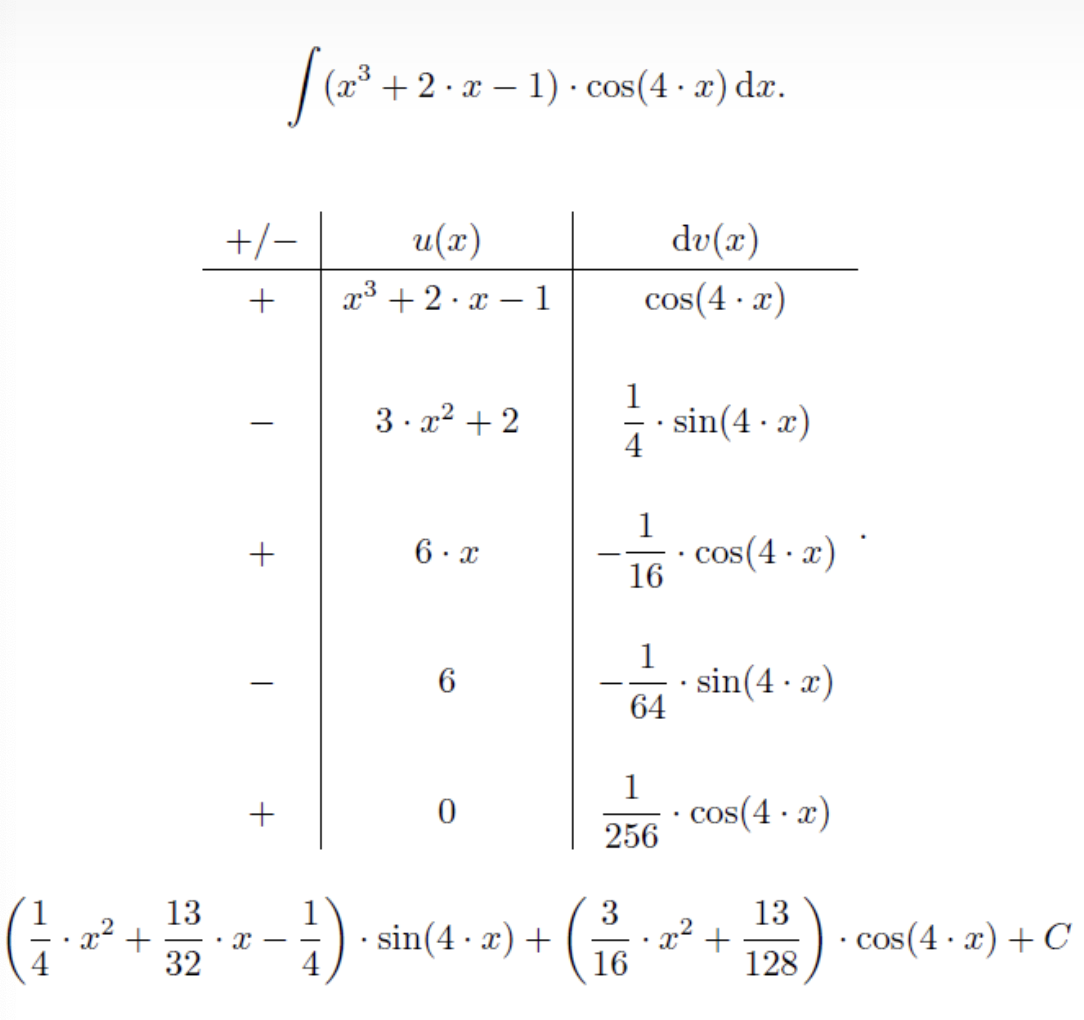
\includegraphics[width=0.6\textwidth]{figs/2022-04-12-10-37-38.png}
	\end{alertblock}
	反、对、幂、三、指的顺序
\end{frame}

\begin{frame}{}
			\begin{alertblock}{分部积分计算定积分$\int_{0}^{\pi}   x^2 (\pi-x)^2   \cos nx dx $}
				$\psi (x) = x^2 (\pi-x)^2$ ,则:\\
				$\displaystyle \begin{array}{lllllllll}
					\psi ' (x) &=  2x(2x - \pi )(x - \pi ) \\
					\psi '' (x) &=  2\pi ^2 -12\pi x+12x^2 \\
					\psi ''' (x) &=  24x -12 \pi \\
					\psi^{(4)} (x) &=  24  \\
				\end{array}$ \\ 
				$\nu^{(4)} (x) = \cos nx$ , 则:\\
				$\displaystyle \begin{array}{lllllllll}
					\nu ''' (x) &= \dfrac{1}{n} \sin nx \\
					\nu '' (x) &= -\dfrac{1}{n^2} \cos nx \\
					\nu ' (x) &= -\dfrac{1}{n^3} \sin nx \\
					\nu (x) &= \dfrac{1}{n^4} \cos nx \\
				\end{array}$ \\ 
			\end{alertblock}
\end{frame}	
		
\begin{frame}
			应用分部积分公式 \\
			$\displaystyle \begin{array}{lllllllll}
				\int\limits_{0}^{\pi}  \psi (x) \nu^{(4)} (x)  dx 
				&= [ \psi \nu''' - \psi' \nu'' + \psi'' \nu' -\psi''' \nu ]|_0 ^\pi +	\int\limits_{0}^{\pi}  \psi^{(4)} (x)  \nu (x)  dx  \\
				&=  [ \psi \nu''' - \psi' \nu'' + \psi'' \nu' -\psi''' \nu ]|_0 ^\pi 
			\end{array}$ \\ 
			* (1)式中:$\int_{0}^{\pi}  \psi^{(4)} (x)  \nu (x)  dx = \frac{24}{n^4} \int_{0}^{\pi}  \cos nx dx =0$ \\
			(2)式中的第1和第3项等于零($\sin nx |_0 ^\pi$) \\
			(3)式中第二项含 $2x(2x - \pi )(x - \pi )|_0 ^\pi$也为零, 因此有:
			\begin{equation*}
				\int\limits_{0}^{\pi}  \psi (x) \nu^{(4)} (x)  dx = [-\psi''' \nu ]|_0 ^\pi =  -\dfrac{12 \pi}{n^4}  [\cos n\pi +1 ]
			\end{equation*}
\end{frame}	

\begin{frame}
	\frametitle{第三类边界条件}
	求第三类边界条件的固有值问题\\
	$\begin{array}{lllllllll}
	III & \begin{cases}
			X'' (x)  + \lambda X =0   ~~,~~ 0<x<L\\
			X' (0) =0, X (L) =0
	\end{cases}\\	
	& \begin{cases}
		\lambda_n=\dfrac{(2n+1)^2 \pi ^2}{4l^2}\\
		X_n(x) = \cos \sqrt{\lambda} x
	\end{cases}\\	
	IV&\begin{cases}
		X'' (x)  + \lambda X =0   ~~,~~ 0<x<L\\
		X (0) =0, X' (L) =0
	\end{cases} \\	
	& \begin{cases}
		\lambda_n=\dfrac{(2n+1)^2 \pi ^2}{4l^2}\\
		X_n(x) = \sin \sqrt{\lambda} x
    \end{cases}\\	
	\end{array}$ \\ 
\end{frame}	

\begin{frame}
	\frametitle{}
	作业-1、求解热传导方程初边值问题\\
	$\begin{array}{lllllllll}
		&\begin{cases}
			u_{t} =a^2u_{xx} ~~,~~ 0<x<l, t>0\\
			u(0,t) =u(l,t)=0 \\
			u(x,0) =x (l-x)
		\end{cases}\\	
		&\begin{cases}
			u_{t} =a^2u_{xx} ~~,~~ 0<x<l, t>0\\
			u_x(0,t) =u_x(l,t)=0 \\
			u(x,0) =x(l-x/2)
		\end{cases} \\	
	\end{array}$ \\ 
	2、求第三类边界条件固有值问题,并求固有函数的正交性\\
	$\begin{array}{lllllllll}
		& \begin{cases}
			X'' (x)  + \lambda X =0   ~~,~~ 0<x<L\\
			X' (0) =0, X (L) =0
		\end{cases}\\	
		&\begin{cases}
			X'' (x)  + \lambda X =0   ~~,~~ 0<x<L\\
			X (0) =0, X' (L) =0
		\end{cases} \\	
	\end{array}$ 	
\end{frame}	

\begin{frame}
	\frametitle{}
	3. 什么是固有值?有何用处?
	\\
	4. 什么是固有函数?与固有值有何关系? 
	\\
	5. 分离变量法的数学思想是什么?
	\\
	6. 什么是叠加原理?与分离变量法有何关系
	\\
	7. 正交性是什么意思?有何用处?
	\\
	8. 较复杂的分部积分法怎么用?	
\end{frame}	


%%%%%%%%%%%%%%%%%%%%%%%%%%%%%%%%%%%%%%%%%%%%%
\section{3.拉普拉斯方程}
\subsection{方程的建立}
\begin{frame}
	\frametitle{方程的建立}
	\begin{exampleblock} {例1、建立拉普拉斯方程}
		对于位于原点的质量为M的质点,试建立其引力势函数
		u(x,y,z,t) 所满足的方程 .
	\end{exampleblock}
	%%\usetikzlibrary {3d} 
	\tikzset{math3d/.style={x={(-0.353cm,-0.353cm)},z={(0cm,1cm)},y={(1cm,0cm)}}}
	\opencutright 
	\def\windowpagestuff{\flushright 
	\begin{tikzpicture}
		\def\k{1.5}
		\draw [ ->] (0,0,0) --  (0,0,2.5)  node[below] {$z$};
		\draw [ ->]  (0,0,0) -- (\k, 0,0)   node[right] {$x$};
		\draw [ ->]  (0,0,0) -- (0,\k, 0)    node[right] {$y$};
		\fill[black!100] (0,0,0) node[right]{$M$} circle(0.8ex);
		\begin{scope}[canvas is zy plane at x=0] \draw (0,0) circle (1cm);
			\draw (-1,0) -- (1,0) (0,-1) -- (0,1);
		\end{scope};
		\begin{scope}[canvas is zx plane at y=0] \draw (0,0) circle (1cm);
			\draw (-1,0) -- (1,0) (0,-1) -- (0,1);
		\end{scope};
		\begin{scope}[canvas is xy plane at z=0] \draw (0,0) circle (1cm);
			\draw (-1,0) -- (1,0) (0,-1) -- (0,1);
		\end{scope};
	\end{tikzpicture}	}
	~~~\hspace*{\fill} \\	
	~~~\hspace*{\fill} \\	
	\begin{cutout} {0}{6cm}{0pt}{5}
		\alert{ 解:}	建立如图坐标系,\\
		在空间任一点(x,y,z)放置试验质点m\\
 		m感受的力为:\\
		{$ \overrightarrow{F} =-G\dfrac{Mm}{r^3} \overrightarrow {r} $ }  ~~,~~ $r=\sqrt{x^2+y^2+z^2}$\\ 
		M激发的引力场强为 \\
		{ $ \overrightarrow{A} =\dfrac{GM}{r^3} \overrightarrow{r} $ }\\
	\end{cutout}
\end{frame}	

\begin{frame}
	\frametitle{}
	取无穷远处场强为零,则引力势为\\
	$\displaystyle  u = -\int_{r}^{\infty} \overrightarrow{A}\cdot d \overrightarrow{r} =- \int_{r}^{\infty} \frac{GM}{r^2} dr =- \frac{GM}{r} $ \\
	即有: $\overrightarrow{A} =-\nabla u$ \\
	封闭球面S内的质量通量为 \\
	$\displaystyle \oint_{S} \overrightarrow{A} \cdot d \overrightarrow{S} = \frac{GM}{r^2} 4\pi r^2 =\int  4\pi G  \rho d\tau$  \\
	由高斯定理可知:\\
	$ \displaystyle \oint_{S} \overrightarrow{A} \cdot d \overrightarrow{S} =\int  \nabla \cdot \overrightarrow{A} d\tau $\\
	因此: 
	\begin{equation*}
		\nabla \cdot \overrightarrow{A} = 4\pi G \rho
	\end{equation*}
	由于 $\nabla \cdot \overrightarrow{A} = \nabla \cdot \left(-\nabla u\right)= -\nabla ^2 u$ \\
	得泊松方程:
	\begin{equation*}
		\nabla ^2 u= -4\pi G \rho
	\end{equation*}	
\end{frame}	

\begin{frame}
	\frametitle{}
	对于无源区域,得拉普拉斯方程
	\begin{equation*}
		\nabla ^2  u =0 
	\end{equation*}
	定义拉普拉斯算子:
	\begin{equation*}
		\triangle  = \nabla ^2 = \frac{\partial ^2}{\partial x^2} +\frac{\partial^2 }{\partial y^2} +\frac{\partial^2  }{\partial z^2}	
	\end{equation*}
	拉普拉斯方程为:
	\begin{equation*}
		\triangle   u =0 
	\end{equation*}
	\begin{block}{Remark}
		拉普拉斯方程和泊松方程是描述各种势场的基本方程。
	\end{block}
\end{frame}	


\subsection{方程的求解}
\begin{frame}
	\frametitle{方程的求解}
	\begin{exampleblock} {例2、求解矩形区域拉普拉斯方程}
		$\displaystyle \begin{cases}
			u_{xx} +u_{yy} =0 ,~~~~ (0<x<a, 0<y<b)\\
			u(x,0)= f_1 (x) ,  u(x,b)= f_2 (x) \\
			u(0,y)= g_1 (y) ,  u(a,y)= g_2 (y) 
		\end{cases}$ \\
	\end{exampleblock}	
	\alert{ 解:}	这是第一类边界条件,但不是零边界条件,可转化为 \\
	$\displaystyle (A) \begin{cases}
		u_{xx} +u_{yy} =0 ,~~~~ (0<x<a, 0<y<b)\\
		u(x,0)= 0,  u(x,b)= 0 \\
		u(0,y)= g_1 (y) ,  u(a,y)= g_2 (y) 
	\end{cases}$ \\
	$\displaystyle (B) \begin{cases}
		u_{xx} +u_{yy} =0 ,~~~~ (0<x<a, 0<y<b)\\
		u(x,0)= f_1 (x) ,  u(x,b)= f_2 (x) \\
		u(0,y)= 0,  u(a,y)= 0 
	\end{cases}$ \\
\end{frame}	

\begin{frame}
	当然,还可以进一步分解成四个边值问题!
	$\displaystyle  (I) \begin{cases}
		u_{xx} +u_{yy} =0 ,~~~~ (0<x<a, 0<y<b)\\
		u(x,0)= 0,  u(x,b)= 0 \\
		u(0,y)= g_1 (y) ,  u(a,y)= 0
	\end{cases}$ \\
	$\displaystyle (II)  \begin{cases}
		u_{xx} +u_{yy} =0 ,~~~~ (0<x<a, 0<y<b)\\
		u(x,0)= 0,  u(x,b)= 0 \\
		u(0,y)= 0,  u(a,y)= g_2 (y) 
	\end{cases}$ \\
	$\displaystyle  (III)  \begin{cases}
		u_{xx} +u_{yy} =0 ,~~~~ (0<x<a, 0<y<b)\\
		u(x,0)= f_1 (x) ,  u(x,b)= 0 \\
		u(0,y)= 0,  u(a,y)= 0 
	\end{cases}$ \\	
	$\displaystyle  (IV)  \begin{cases}
		u_{xx} +u_{yy} =0 ,~~~~ (0<x<a, 0<y<b)\\
		u(x,0)= 0,  u(x,b)= f_2 (x) \\
		u(0,y)= 0,  u(a,y)= 0 
	\end{cases}$ \\	
\end{frame}		

\begin{frame}
	\frametitle{}
	 以方程(I)为例求解\\
	$\displaystyle \begin{cases}
		u_{xx} +u_{yy} =0 ,~~~~ (0<x<1, 0<y<1)\\
		u(x,0)= 0,  u(x,1)= 0 \\
		u(0,y)= g_1 (y) =\sin \pi y,  u(1,y)= 0
	\end{cases}$ \\
	\alert{ 解:}	设有 	$ u(x,y)=X(x) Y(y)$ ,代回原方程,得
	\begin{equation*}
		X~^{''}(x)Y(y) +X(x)Y~^{''}=0
	\end{equation*}
	\begin{equation*}
		-\frac{X~^{''}}{X}=\frac{Y~^{''} }{Y} =-\lambda 
	\end{equation*}	
	得两个常微分方程:
\end{frame}	

\begin{frame}
	\frametitle{}	
	方程(1):\\
	$\displaystyle  \begin{cases}
		Y~^{''} +\lambda Y=0  ~~,~~ 0<y<1\\
		Y(0)=0 ~~,~~Y(1)=0 
	\end{cases}$ \\	
	方程(2):\\
	$\displaystyle  \begin{cases}
		X~^{'} -\lambda X=0  ~~,~~ 0<x<1 \\
		X(0)=\sin \pi y~~,~~X(1)=0 
	\end{cases}$ \\	\vspace{0.3em}
	方程(1)是一类条件零边界固有值问题,公式:\\
	固有值:$\displaystyle  \lambda~_n=\frac{n^2\pi~^2}{l~^2} =n^2\pi~^2$ \\ 
	固有函数: $\displaystyle  Y~_n= \sin \frac{n\pi~}{l} y = \sin n \pi y $ \\	
\end{frame}	

\begin{frame}
	\frametitle{}	
	解方程II : 
	代入$\lambda_n$, 得:
	$\displaystyle  X~^{''} - n^2\pi~^2~X=0 $ \\
	特征方程有两相异实根,通解为: \\ 
	\begin{equation*}
		X_n(x)=C_n exp(n\pi x )+ D_n exp(-n\pi x )
	\end{equation*}	
	结合(1)(2),方程(I)的基本解:\\ 
	$\displaystyle \begin{array}{llll}
		u_n(x,y) &=& [C_n exp(n\pi x )+ D_n exp(-n\pi x )] \sin (n \pi y)  \\ 
		&=& [a_n \cosh (n\pi x )+ b_n \sinh(n\pi x ) ]\sin (n \pi y)  \\ 
	\end{array}$ \\
	叠加解:
	\begin{equation*}
		u(x, y)   = \sum\limits_{n=1}^{\infty }  [a_n \cosh (n\pi x )+ b_n \sinh (n\pi x ) ] \sin (n \pi y)  
	\end{equation*}	
\end{frame}	

\begin{frame}
	\frametitle{}	
	代入定解条件:$ u(0,y)=0$, 得 \\
	$ \sum\limits_{n=1}^{\infty }  a_n  \sin (n \pi y) =0 $ ,=> $ a_n=0$ \\
	因此:\\
	$	u(x,y)    = \sum\limits_{n=1}^{\infty }  b_n \sinh (n\pi x )  \sin (n \pi y)  $ \\ 
	代入定解条件:$u(1,y) = \sin \pi y $, 得
	\begin{equation*}
		u(1,y)    = \sum\limits_{n=1}^{\infty }  b_n \sinh (n\pi )  \sin (n \pi y)  = \sin \pi y
	\end{equation*}
	正交性,得:$ b_1\sinh\pi =1,~~ b_n=0~,~ (n>1)$	\\ 
	原方程得解:
	\begin{equation*}
		u(x,y)    = \dfrac{\sinh \pi x}{\sinh \pi}  \sin ( \pi y) 
	\end{equation*}	
\end{frame}	

\begin{frame}
	\frametitle{}	
	同理,可以求出其他三个方程的解,最终进行线性叠加,得到矩形区域拉普拉斯方程的解:
	\begin{equation*}
		u(x,y)    = u_I (x,y)  +   u_{II}(x,y)  + u_{III}(x,y)  + u_{IV}(x,y)  
	\end{equation*}	
\end{frame}	

\begin{frame}
	\frametitle{}	
	\begin{block}	{注: 双曲函数:}		
		$\displaystyle \begin{cases}
			&\sinh(x) = -i \sin(ix) = \frac{e^x -e^{-x}}{2} \\
			&\cosh(x) = \cos(ix) = \frac{e^x +e^{-x}}{2} 
		\end{cases}$ 
	\end{block}
	\begin{center}
	    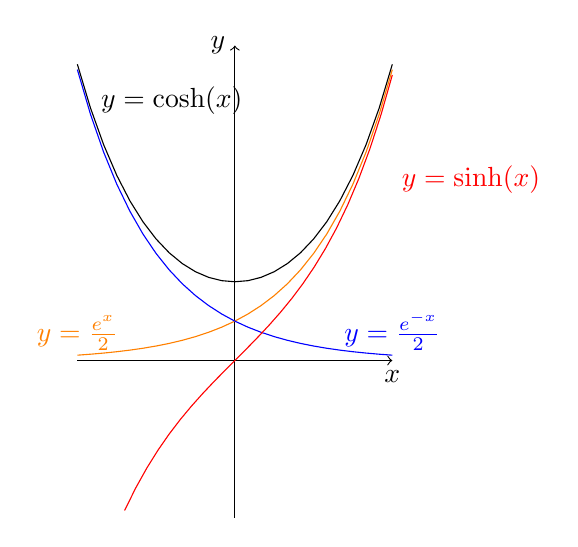
\begin{tikzpicture} 
    	\draw[->] (-2,0) -- (2,0) node[below] {$x$};
    	\draw[->] (0,-2) -- (0,4) node[left] {$y$};
    	\draw[orange, domain= -2:2]  plot (\x, {  exp(\x) * 0.5  } ) ;
    	\draw[orange]  (-2,0) node[above] {$y=\frac{e^ x}{2}$};
    	\draw[ blue, domain= -2:2]  plot (\x, {  exp(-\x) * 0.5  } );
    	\draw[blue]  (2,0) node[above] {$y=\frac{e^ {-x}}{2}$};
    	\draw[red, domain= -1.4:2]  plot (\x, {  exp(\x) * 0.5 -  exp(-\x) * 0.5 } ) ;
    	\draw[red]  (3,2) node[above] {$y=\sinh(x)$};
    	\draw[black, domain= -2:2]  plot (\x, {  exp(\x) * 0.5 +exp(-\x) * 0.5 } );
    	\draw[black]  (-0.8,3) node[above] {$y=\cosh(x)$};
	    \end{tikzpicture} 
	\end{center}
\end{frame}	

\subsection{区域边界条件}
\begin{frame}
	\frametitle{圆域拉普拉斯方程}	
	拉普拉斯算符在不同坐标系中的具体形式\\  \vspace{0.6 cm}	
	直角坐标~ $(x,y,z): $	{ 	$ \displaystyle  \nabla ^{2}  = \frac{\partial ^2}{\partial x^2} +\frac{\partial^2 }{\partial y^2} +\frac{\partial^2  }{\partial z^2}$}\\ 	
	球坐标~ $	(r,\theta, \varphi )$ :
	{ 	$ \displaystyle  \nabla ^{2} =\frac{1}{r^2} \frac{\partial }{\partial r} (r^2\frac{\partial }{\partial r} )+
		\frac{1}{r^2 \sin \theta  } \frac{\partial }{\partial \theta } (\sin \theta \frac{\partial }{\partial \theta } )
		+\frac{1}{r^2 \sin^2 \theta  } \frac{\partial^2}{\partial\varphi ^2}$ } \\ 	
	极坐标~ $	(r,\theta)$ :
	{ 	$ \displaystyle  \nabla ^{2} =\frac{\partial ^2 }{\partial r^2 } +\frac{1}{r } \frac{\partial }{\partial r } +
		\frac{1}{r^2 } \frac{\partial ^2 }{\partial \theta ^2 } $ }\\ 		
\end{frame}	
	
\begin{frame}	
	\begin{exampleblock} {例3、求圆域拉普拉斯方程}
	{ $  \displaystyle  \left \{ 
	\begin{array}{cc}
		\displaystyle {	\frac{\partial^2 u }{\partial r^2 } +\frac{1}{r } \frac{\partial u }{\partial r } +
			\frac{1}{r^2 } \frac{\partial ^2 u }{\partial \theta ^2
		} } =0, ~~ 0<r<r_0\\
		\\
		u(r_0,\theta )=f(\theta ) ,~~~~~~~~~~~~ 0<\theta <2\pi 
	\end{array}
	\right. $}  
	\end{exampleblock}	
	\alert{ 解:}	 
	方程可分离变量,令 $\displaystyle  u(r,\theta)=R(r) \Theta(\theta)$,代回原方程  \\ 
	{ $\displaystyle  R''\Theta +\dfrac{1}{r^2} R\Theta '' +\dfrac{1}{r}R'\Theta=0 $} \\ 
	{ $\displaystyle  \dfrac{r^2R''+rR'}{R}=-\dfrac{\Theta '' }{\Theta} =\lambda $} \\ 
	得两常微分方程:
\end{frame}	

\begin{frame}	
	I、 $\displaystyle 	\Theta '' + \lambda \theta =0 $  \\ 
	定解条件:$\displaystyle 	\Theta(\theta +2 \pi )=\Theta (\theta)  $  \\ 
	II、$\displaystyle  r^2 R'' +r R' -\lambda R =0 $  \\   \vspace{0.6 cm}	
	
	解方程I:  根据以前的分析,在 $\lambda > 0 $ 时,有通解\\ 
	{ $\displaystyle  \Theta(\theta)=A\cos \sqrt{\lambda } \theta+B\sin \sqrt{\lambda }\theta$}\\ 
	由定解条件:$\displaystyle 	\Theta(2 \pi )=\Theta (0)~,~~ 	\Theta' (2 \pi )=\Theta' (0)  $ 得方程: \\ 
	$ \left [
	\begin{array}{lll}
		\cos (\sqrt {\lambda} 2\pi )-1  & \sin (\sqrt {\lambda} 2\pi )\\
		-\sin (\sqrt {\lambda} 2\pi ) & \cos (\sqrt {\lambda} 2\pi )-1
	\end{array} \right] 
	\left [
	\begin{array}{lll}
		A\\
		B
	\end{array} \right] 
	=
	\left [
	\begin{array}{lll}
		0\\
		0
	\end{array} \right]
	$ \\
	系数行列式为零,得\\
	$(\cos (\sqrt {\lambda} 2\pi )-1 ) ^2 + \sin ^2 (\sqrt {\lambda} 2\pi ) =0$ \\ 
\end{frame}	

\begin{frame}
	$\cos (\sqrt {\lambda} 2\pi)=1$   \\ 	
	固有值:$\lambda _n =n^2 ~,~~ (n=0,1,2,...)$  \\ 
	固有函数:$\displaystyle  \Theta(\theta)=A_n\cos n \theta +B_n \sin n \theta $\\   \vspace{0.6cm}

	解方程II:
	{$\displaystyle  r^2 R'' +r R' -\lambda R =0 $  } \\ 
	把$\lambda_n =n^2 $代入, 得 \\ 
	{$\displaystyle  r^2 R'' +r R' -n^2R =0 $  } \\ 
	这是欧拉方程:令 $ r=exp(t) $ ,有 $t=\ln r$, 求导 \\ 
	$ \displaystyle \frac{dR}{dr} =\frac{dR}{dt} \frac{dt}{dr} =\frac{1}{r} \frac{dR}{dt} $ \\ 
	$ \displaystyle \frac{d^2R}{dr^2} =-\frac{1}{r^2}\frac{dR}{dt} + \frac{1}{r} \frac{d}{dr} (\frac{dR}{dt} )$ \\ 
	$ \displaystyle \frac{d^2R}{dr^2} =\frac{1}{r^2} (\frac{d^2R}{dt^2}-\frac{dR}{dt} )$ \\ 		
\end{frame}	

\begin{frame}	
	代回方程,得:\\ 
	$ \displaystyle   \dfrac{d^2R}{dt^2} -n^2 R =0 $ \\ 
	由特征方程有两相异实根,得通解:\\ 
	$ R=C_nexp(nt)+D_n exp(-nt) $\\
	把 $t=\ln r$ 代回,得\\
	$R=C_n r^n +D_nr^{-n}$ \\ 
	第二项发散,应删除,得\\
	$R= C_n r^n,  ~~ (n=0,1,2,......) $		\\
	基本解:\\ 
	$\begin{array}{llll}
		u_n(r,\theta) &=&  r^n(a_n \cos n\theta +b_n \sin n \theta )   \\ 
	\end{array}$ \\ 	
\end{frame}	

\begin{frame}	
	叠加解:\\ 
	$\begin{array}{llll}
		u(r, \theta) &=& \dfrac{1}{2} a_0 +\sum\limits_{n=1}^{\infty }r^n (a_n  \cos n\theta +b_n \sin n \theta ) 
	\end{array}$ \\ 
	代入定解条件:$ u(r_0,\theta)=f (\theta) =  \dfrac{1}{2} a_0 +\sum\limits_{n=1}^{\infty } (a_n\cos n\theta +b_n \sin n \theta ) r_0^n $\\ 
	系数公式:\\ 
	$  \displaystyle  a_n = \dfrac{1}{r_0 ^n \pi }  \int\limits_{0}^{2\pi} f(\theta) \cos n \theta d\theta $ \\ 
	$  \displaystyle  b_n = \dfrac{1}{r_0 ^n \pi }  \int\limits_{0}^{2\pi} f(\theta) \sin n \theta d\theta $  \\ 	
\end{frame}	

\begin{frame}	
	\begin{exampleblock} { 例4、求解如下边值问题}
	{ $  \displaystyle  \left \{ 
	\begin{array}{cc}
		\displaystyle {	\dfrac{\partial^2 u }{\partial r^2 } +\dfrac{1}{r } \dfrac{\partial u }{\partial r } +
		\dfrac{1}{r^2 } \dfrac{\partial ^2 u }{\partial \theta ^2
		} } =0, ~~ 0<r<r_0\\
		\\
		u(r_0,\theta )=A\cos(\theta),~~~~~~~~~ 0<\theta <2\pi 
	\end{array}
	\right. $}  
	\end{exampleblock}	
	\alert{ 解:}	 求系数:\\
	$  \displaystyle  a_1 = \dfrac{1}{r_0 ^1 \pi }  \int\limits_{0}^{2\pi} A\cos(\theta) \cos  \theta d\theta  $ \\ 	
	\hspace{0.8cm}$  \displaystyle  = \dfrac{A}{r_0  \pi }  \int\limits_{0}^{2\pi} \cos ^2 (\theta)  d\theta  = \frac{A}{r_0 \pi }  \int\limits_{0}^{2\pi} (1+\cos2\theta) d\theta$ = $\dfrac{2A}{r_0}$ \\ 
	$  \displaystyle  a_n = \dfrac{1}{r_0 ^n \pi }  \int\limits_{0}^{2\pi} A\cos(\theta) \cos n \theta d\theta =0~,~ (n\ne 1)$ \\ 
\end{frame}	

\begin{frame}	
	$  \displaystyle  b_n = \dfrac{1}{r_0 ^n \pi }  \int\limits_{0}^{2\pi} A\cos(\theta) \sin n \theta d\theta =0 $  \\ 
	叠加解:\\
	$\begin{array}{llll}
		u(r, \theta) &=& \dfrac{1}{2} a_0 +\sum\limits_{n=1}^{\infty } (a_n r^n\cos n\theta +b_n \sin n \theta )  \\
		&=& \dfrac{1}{2} a_0+ a_1 r\cos \theta \\
		&=&  \dfrac{A}{r_0} r \cos \theta 
	\end{array}$ \\ 
	\begin{block}{Remark}
		若将边界条件修改为: $A \cos 2\theta$ ,或 $A \sin 2\theta $ ,解会如何变化?
	\end{block}
\end{frame}	

\begin{frame}	
%	\frametitle{作业} 
	作业:
	1、求解固有值问题\\ 
	$\begin{array}{lllllllll}
		& \begin{cases}
			Y~^{''} +\lambda Y=0  ~~,~~ 0<y<2\pi \\
			Y(0) =Y(2\pi) , ~~ Y'(0) =Y'(2\pi)
		\end{cases}\\	
	\end{array}$ \\ 
	2、求解圆域边值问题\\
	$\displaystyle  \begin{array}{lllllllll}
	&\begin{cases}
		\dfrac{\partial^2 u }{\partial r^2 } +\dfrac{1}{r } \dfrac{\partial u }{\partial r } +
		\dfrac{1}{r^2 } \dfrac{\partial ^2 u }{\partial \theta ^2  } =0, ~~ 0<r<1\\
		u(1,\theta)= A\cos 2 \theta +B \cos 4 \theta \\	
	\end{cases} \\	
	\end{array}$ \\ 
	3、求解矩形域边值问题\\
	$\begin{array}{lllllllll}
		& \begin{cases}
			u_{xx} +u_{yy} =0 ,~~~~ (0<x, y<1)\\
			u(x,0)= u(0,y)=u(x,1)= 0 \\
			u(1,y)= \sin 2\pi y
		\end{cases}\\	
		&\begin{cases}
			u_{xx} +u_{yy} =0 ,~~~~ (0<x, y<1)\\
			u(1,y)= u(0,y)=u(x,0)= 0 \\
			u(x,1)= \sin n\pi x
		\end{cases} \\	
	\end{array}$ \\ 	
\end{frame}

\begin{frame}
	\frametitle{课外读物和思考}
	了解和学习三大偏微分方程的各种解法:\\
	《Partial Differential Equations》- 作者: Lawrence C. Evans \\
	《An Introduction to Partial Differential Equations》- 作者: M. Renardy R. C. Rogers
\end{frame}
%%%%%%%%%%%%%%%%%%%%%%%%%%%%%%			

%%%%%%%%%%%%%%%%%%%%%%%%%%%%%%%%%%%%%%%%%%%%%%%%%
\begin{frame}
		\frametitle{}
		\Background[1] 
	    \begin{center}
		{ {\Huge 第三章~~薛定谔方程 (I)\\(6学时)}}
	    \end{center}    
\end{frame}
%%%%%%%%%%%%%%%%%%%%%%%%%%%%%%%%%%%%%%%%%%%%%

\section{1.薛定谔方程基础}
\subsection{薛定谔方程}
\begin{frame}
	\frametitle{}  
	\begin{block}	{量子力学有关波函数的基本结论}
	\begin{itemize}
		\item 	波函数$\Psi$完全描述体系的状态,
		\item 	波函数的模方与粒子出现的概率成比例,$\omega \sim |\Psi|^2$
		\item 	波函数的演化服从薛定谔方程 : $\hat{E} \Psi = \hat{H}  \Psi $ 
	\end{itemize}
	薛定谔方程是量子力学基本方程,与牛顿力学的牛顿第二定理地位相当
	\end{block}	
\end{frame}

%%%%%%%%%%%%%%%%%%%%%%%%%%%%%%%%%%%%%%%%%%%%%
\begin{frame}
	\frametitle{方程的建立}
	\begin{alertblock} {可能思路}  
		\begin{itemize}
			\Item 	\textbf{1:}  最小作用量原理 $\int\limits_{t_1}^{t_2} \delta L d t =0 $\\ 
			\Item 	\textbf{2:}  波粒二象性\\ 
			~\\ 
			\Item 	\textbf{3:}  基本假设,不能从现有理论推导\\
            ~\\ 
            \begin{quote}
            "It is not possible to derive it from anything you know. It came out of the \alert{\faHeartbeat} of Schr$\ddot{o}$dinger"\\
            \rightline{$\cdots$ R. P. Feynman \hspace{3em}}   
            \end{quote}
		\end{itemize}
	\end{alertblock}
\end{frame}
\begin{frame}
	\frametitle{含时薛定谔方程}
	标准形式:    
	 \begin{equation*}
		i\hbar \frac{\partial }{\partial t} \Psi (\overrightarrow{r},t ) =\left [ -\frac{\hbar^2}{2\mu }\nabla ^2 + V(\overrightarrow{r},t ) \right ]\Psi (\overrightarrow{r}, t ) 
	\end{equation*}
	若取 $ \displaystyle  i\hbar \frac{\partial }{\partial t} ~~\to ~~ \hat{E} ~~, ~~  -\frac{\hbar^2}{2\mu }\nabla ^2 + V(\vec{r},t ) ~~\to ~~ \hat{H} $ \\
	算符形式:   \\ 
	\begin{equation*}
		\hat{E} ~ \Psi (\overrightarrow{r},t )  = \hat{H} ~ \Psi (\overrightarrow{r},t )  
	\end{equation*}
\end{frame}

\subsection{分离变量}

\begin{frame}
	\frametitle{分离变量}
	\begin{alertblock} {薛定谔方程$\hat{E} \Psi = \hat{H}  \Psi $ 为什么难求解?因为很难分离变量!}
		~~\\
		多粒子体系的波函数:
		\begin{equation*}
			\Psi (\vec{r_1},\vec{r_2},...,\vec{r_n},t )
		\end{equation*}		
		多粒子体系的哈密顿量:
		\begin{equation*}
			\hat{H} ~=\sum_{i=1}^{n} -\frac{\hbar^2}{2\mu }\nabla ^2 _i + \sum_{i=1}^{n} V(\vec{r_i},t) + \sum_{i,j=1, i\ne j}^{n}  U(\vec{r_i},\vec{r_j}) 
		\end{equation*}	
		有可能分离变量吗?条件呢?
	\end{alertblock}	
\end{frame}

\begin{frame}
\frametitle{分离变量(1)->固有值问题->定态薛定谔方程}
	若势函数$V(\vec{r},t ) $不显含时间$t$,时间变量可分离 \\ \vspace{0.3cm}
	方程: { $ \displaystyle i \hbar \frac{\partial }{\partial t} \Psi (\vec{r},t ) =\left [- \frac{\hbar^2}{2\mu }\nabla ^2 + V(\vec{r}) \right ]\Psi (\vec{r},t ) $}  \\  \vspace{0.3cm}
	\alert{解:}  设  $\Psi (\vec{r},t )  = \Psi (\vec{r} ) f(t) $ , 代回方程 \\ \vspace{0.6em}
	{ $ \displaystyle i\hbar \Psi (\vec{r})  \frac{\partial }{\partial t} f(t)=f(t) \left [ -\frac{\hbar^2}{2\mu }\nabla ^2 + V(\vec{r}) \right ]\Psi (\vec{r}) $}  \\ 	
	{ $ \displaystyle i\hbar \frac{1}{f(t)}  \frac{\partial }{\partial t} f(t)= \frac{1}{\Psi (\vec{r}) } \left [ -\frac{\hbar^2}{2\mu }\nabla ^2 + V(\vec{r}) \right ]\Psi (\vec{r}) =E $}  \\ 	
\end{frame}

\begin{frame}
	\frametitle{}
	得两个微分方程:\\  \vspace{0.3cm}
	I、演化问题(方程)  \[ \displaystyle  i\hbar \frac{1}{f(t)}  \frac{\partial }{\partial t} f(t)=E \]   
	解方程,得:$\displaystyle  f(t) =e^{-iEt/\hbar}$ \\  \vspace{0.6cm}
	II、固有值问题(定态薛定谔方程) \[\displaystyle   \left [ -\frac{\hbar^2}{2\mu }\nabla ^2 + V(\vec{r}) \right ]\Psi (\vec{r}) =E \Psi (\vec{r})  \]   
	算符形式:\[   \hat{H} \Psi (\vec{r}) =E \Psi (\vec{r})    \] 
	哈密顿量决定固有值问题(定态薛定谔方程)求解难度!	
\end{frame}

\begin{frame}
	\frametitle{分离变量(2)->单粒子定态薛定谔方程}
	多粒子体系的定态薛定谔方程:   
	\begin{equation*}
		\left [ \sum\limits_{i=1}^{n} \hat{H}_i + \sum_{i,j=1, i\ne j}^{n}  U(\vec{r_i},\vec{r_j}) \right ]	\Psi (\vec{r_1},\vec{r_2},...,\vec{r_n})=E 	\Psi (\vec{r_1},\vec{r_2},...,\vec{r_n})
	\end{equation*}		
	\alert{解:}  	对于无相互作用体系, 
	有$ U(\vec{r_i},\vec{r_j}) =0 $,\\
	 $ \hat{H}= \sum\limits_{i=1}^{n} (-\dfrac{\hbar^2}{2\mu }\nabla ^2 _i + V(\vec{r_i})) =\sum\limits_{i=1}^{n} \hat{H}_i \qquad (1)$\\   \vspace{0.3cm}
	方程可进一步分离变量!令 : \\
	 $\displaystyle \begin{cases}
	   	\Psi (\vec{r_1},\vec{r_2},...,\vec{r_n}) = \Psi (\vec{r_1}) \Psi (\vec{r_2})...\Psi (\vec{r_n}) \qquad (2) \\
		E= E_1+ E_2 + ... + E_n=\sum\limits_{i=1}^{n} \hat{E}_i \qquad (3)
	\end{cases}$ \\ \vspace{0.3em}
 	把(1)(2)(3)代回原方程
\end{frame}

\begin{frame}
	\frametitle{}
	获得如下方程
	\[ \sum\limits_{i=1}^{n} \hat{H}_i\Psi (\vec{r_1}) \Psi (\vec{r_2})...\Psi (\vec{r_n})= \sum\limits_{i=1}^{n} \hat{E}_i\Psi (\vec{r_1}) \Psi (\vec{r_2})...\Psi (\vec{r_n}) \]
	进一步简化,得单粒子定态薛定谔方程组\\
	$\displaystyle \begin{cases}
		\hat{H}_1\Psi (\vec{r_1})=E_1 \Psi (\vec{r_1})  \\  
		\hat{H}_2\Psi (\vec{r_2})=E_2 \Psi (\vec{r_2})  \\
		\dots\\
		\hat{H}_n\Psi (\vec{r_n})=E_n \Psi (\vec{r_n})  \\
	\end{cases}$ \\	
\end{frame}

\begin{frame}
	\frametitle{分离变量(3)->一维定态薛定谔方程} 
	单粒子定态薛定谔方程标准型
	\begin{equation*}
		\left [ -\dfrac{\hbar^2}{2\mu }\nabla ^2 + V(x,y,z) \right ]\Psi (x,y,z) =E \Psi (x,y,z)  
	\end{equation*}		
	\alert{解:} 若势函数 $ V(x,y,z)=V_1(x)+V_2(y)+V_3(z) $,则  $ \hat{H}=\hat{H}(x)+\hat{H}(y)+\hat{H}(z) $\\
	进一步分离变量:设  $$\Psi (x,y,z)  = \Psi_1 (x)\Psi_2 (y) \Psi_3 (z), \qquad  E= E_x+ E_y+E_z $$ \\
	代回, 得一维薛定谔方程(组)
	$\displaystyle \begin{cases}
		\hat{H}(x)\Psi_1 (x)=E_x \Psi_1 (x) \\
		\hat{H}(y)\Psi _2 (y)=E_y \Psi _2 (y)  \\
		\hat{H}(z)\Psi _3 (z)=E_z \Psi _3 (z) 
	\end{cases}$ \\	
\end{frame}

\begin{frame}
	\frametitle{}	
	如果势函数 $$ V(x,y,z)=V(r,\theta,\varphi) =V_1(r)+V_2(\theta)+V_3(\varphi) $$
	令  $$ \hat{H}=\hat{H}(r)+\hat{H}(\theta)+\hat{H}(\varphi) $$
	分离变量得一维薛定谔方程:\\
	$\displaystyle \begin{cases}
		\hat{H}(r)\Psi_1 (r)=E_r \Psi_1 (r) \\
		\hat{H}(\theta)\Psi _2 (\theta)=E_\theta \Psi _2 (\theta)  \\
		\hat{H}(\varphi)\Psi _3 (\varphi)=E_\varphi \Psi _3 (\varphi) 
	\end{cases}$ \\	
\end{frame}

%%%%%%%%%%%%%%%%%%%%%%%%%%%%%%%%%%%%%%%%%%%%%
\section{2.无限深势阱}

\begin{frame}
	\frametitle{}
	\begin{exampleblock} {例1、	一维无限深势阱I}
	一粒子处于如下一维无限深势阱,求解含时薛定谔方程\\
 	{ $ \displaystyle 
	V(x)=\left \{ 
	\begin{array}{cccc}
		0	~~ ~~ 0<x<a \\  
		+\infty ~~x<0, x>a\\
	\end{array}
	\right.
	$} \\
	\end{exampleblock} %2
	\alert{解:} 	势函数不显含时间t,含时薛定谔方程可分离变量,时间演化方程已求得(见前),现求定态薛定谔方程:\\
	{  $ \displaystyle 
	\left \{ 
	\begin{array}{cccc}
		\left [ -\dfrac{\hbar^2}{2\mu} \dfrac{\mathrm{d} ^2}{\mathrm{d} x^2} +0 \right ]\Psi(x)=E\Psi(x)  ~~ ~~ 0<x<a,~~~~~~~~ (1)  \\ 
		\\	
		\left [ -\dfrac{\hbar^2}{2\mu} \dfrac{\mathrm{d} ^2}{\mathrm{d} x^2} +\infty \right ]\Psi(x)=E\Psi(x)  ~~ ~~ x<0,~ x>a ~~~~~(2)  \\
	\end{array}
	\right.
	$} \\
\end{frame}

\begin{frame}
	\frametitle{}
	方程(2):解为  $\Psi(x) = 0$ \\ 
    方程(1):令 $ k^2= \dfrac{2\mu E}{\hbar ^2} $, 方程是如下边值问题:  \\ 
	{ $ \displaystyle 
		\begin{cases}
			\Psi''(x) + k^2	\Psi(x)=0  \\
			\Psi(0)=0~,~~ \Psi(a)=0 ~~~~~
		\end{cases}
		$} \\  \vspace{0.3cm}
    特征方程有两虚根,通解为:\\
     	\begin{equation*}
  			\Psi(x) = A\cos(kx) +B\sin(kx) 
    	\end{equation*}
    取$x=0, x=a$,  代入上式,由零边值条件得:\\
   	\hspace{2cm} $A=0, ~~~~ \sin ka =0$  \\  \vspace{0.3cm}
	有:$ka=n\pi  \to  k=\dfrac{n\pi}{a} = \sqrt{\dfrac{2\mu E}{\hbar ^2}}$    \\ 
\end{frame}

\begin{frame}
	\frametitle{}
	固有值(能级):{ $E_n = \dfrac{n^2\pi^2\hbar^2}{2\mu a^2} (n=1,2,3,...)$} \\
	能级间隔:  $\triangle E = E_{n+1}-E_n=\dfrac{\pi^2 \hbar^2}{2\mu a^2} (2n+1)$ \\ 
	固有函数: $ \Psi_n(x) = B_n\sin(\dfrac{n\pi}{a}x)  = \sqrt{\dfrac{2}{a}} \sin(\dfrac{n\pi}{a}x)$ \\ 
	\alert{归一化}: $ \int \limits_{0}^{a}  \Psi_n ^*(x)  \Psi_n(x)dx = \int \limits_{0}^{a}  |B_n| ^2 \sin^2(\dfrac{n\pi}{a}x) dx =1$  \\ 
	系数:$B_n=\sqrt{\dfrac{2}{a}}$ \\ 
	解函数: \\
	{  $ \displaystyle 
		\Psi_n(x,t)= \left \{ 
		\begin{array}{cccc}
			\sqrt{\dfrac{2}{a}} \sin(\dfrac{n\pi}{a}x) e^{-\dfrac{i}{\hbar} E_n t} ~~~~   0<x<a \\
			0 ~~~~~~~~~~~~~~~~~~~~~~~ x<0,x>a  
		\end{array}
		\right.
		$} \\	
\end{frame}

\begin{frame}
	\frametitle{}
  叠加解:
	  \[\Psi_(x,t)= A_n \psi_n(x,t)\]

  (1)给出定解条件,如何求$A_n$ \\ 
  (2)势阱有变化.如何解方程\\ \vspace*{0.6em}
	 {$ \displaystyle 
   V(x)=\left \{ 
   \begin{array}{cccc}
	   0+1	~~ ~~ 0<x<a \\  
	   +\infty ~~x<0, x>a\\
   \end{array}
   \right.
   ;$} \\ \vspace*{0.3em}
   {$ \displaystyle  V(x)=\left \{ 
	  \begin{array}{cccc}
		  0	~~ ~~ -a<x<a \\  
		  +\infty ~~x<-a, x>a\\
	  \end{array}
	  \right.
  ;$}\\ \vspace*{0.3em}
  {$ \displaystyle   V(x)=\left \{ 
	  \begin{array}{cccc}
		  0	~~ ~~ -\frac{a}{2}<x<\frac{a}{2} \\  
		  +\infty ~~x<-\frac{a}{2}, x>\frac{a}{2}\\
	  \end{array}
	  \right.
   $} \\
\end{frame}

\begin{frame}
	\frametitle{}
	%\usetikzlibrary {datavisualization.formats.functions} 
	\begin{center}
	\begin{tikzpicture}[baseline, scale=.6]
	\datavisualization [ scientific axes, 
		visualize as smooth line/.list={sin,cos,tan}, style sheet=strong colors,
		style sheet=vary dashing,
		sin={label in legend={text=$\Psi_1$}}, 
		cos={label in legend={text=$\Psi_2 $}}, 
		tan={label in legend={text=$\Psi_3 $}}, 
		data/format=function ]
		data [set=sin] {
			var x : interval [0:1];
			func y = sin(pi* \value x r ) * 1.414;
		}
		data [set=cos] {
			var x : interval [0:1];
			func y = sin(2*pi* \value x r ) * 1.414;
		}
		data [set=tan] {
			var x : interval [0:1];
			func y = sin(3*pi* \value x r ) * 1.414;
		};
	\end{tikzpicture} \\ \vspace{0.3cm}
	\end{center}
	\begin{center}
	\begin{tikzpicture}[baseline, scale=.6]
		\datavisualization [ scientific axes, 
		visualize as smooth line/.list={sin,cos,tan}, style sheet=strong colors,
		style sheet=vary dashing,
		sin={label in legend={text=$|\Psi_1|^2$}}, 
		cos={label in legend={text=$|\Psi_2|^2$}}, 
		tan={label in legend={text=$|\Psi_3|^2$}}, 
		data/format=function ]
		data [set=sin] {
			var x : interval [0:1];
			func y = sin(pi* \value x r ) *sin(pi* \value x r ) *2;
		}
		data [set=cos] {
			var x : interval [0:1];
			func y = sin(2*pi* \value x r ) *sin(2*pi* \value x r ) *2;
		}
		data [set=tan] {
			var x : interval [0:1];
			func y = sin(3*pi* \value x r ) * sin(3*pi* \value x r ) *2;
		};
	\end{tikzpicture}
	\end{center}
\end{frame}

\begin{frame}
	\frametitle{}
	\begin{exampleblock} {例2、无限深势阱II}
		设有一粒子处于如下一维无限深势阱中,求解薛定谔方程\\
		{ $ \displaystyle 
			V(x)=\left \{ 
			\begin{array}{cccc}
				0	~~ ~~ |x|<\dfrac{a}{2} \\  
				+\infty ~~|x|>\dfrac{a}{2}\\
			\end{array}
			\right.
		$} \\
	\end{exampleblock}
	\alert{解:} 	势函数与上例存在平移关系, 令$x' =x+a/2$\\
	有:  $  \sin(\dfrac{n\pi}{a}x') =\sin(\dfrac{n\pi}{a} (x+a/2)) $ \\
	\hspace{2cm}$=\sin \dfrac{n\pi}{a} x \cos \dfrac{n\pi}{2} + \cos \dfrac{n\pi}{a} x \sin \dfrac{n\pi}{2}  $ \\ 
	n为偶数: $E_{2m} = \dfrac{2m^2\pi^2\hbar^2}{\mu a^2} $\\
	\hspace{2cm}$ \Psi_{2m}(x)= B_{2m} \sin(\dfrac{2m\pi}{a}x) $,   \\
\end{frame}

\begin{frame}
	\frametitle{}
	n为奇数:  $E_{2m+1} = \frac{(2m+1)^2\pi^2\hbar^2}{2\mu a^2} $ \\
	\hspace{2cm}$ \Psi_{2m+1}(x)= B_{2m+1} \cos(\dfrac{(2m+1)\pi}{a}x) $,  \\
	归一化,求系数 ... \\	 \vspace{0.6cm}	
	\textbf{如果把势阱宽改为2a}, 直接求解, 可得: \\
	固有值(能级):{ $E_n = \dfrac{n^2\pi^2\hbar^2}{8\mu a^2} (n=1,2,3,...)$} \\
	固有函数: $ \Psi_n(x)= \sqrt{\dfrac{2}{a}} \sin(\dfrac{n\pi}{a}(x+a)) $ \\  \vspace{0.6cm}	
	比较两种解之间的关系!	明确势阱平移与伸缩后解的写法。
\end{frame}

\begin{frame}
	\frametitle{}
	\begin{exampleblock} {例3、无限深势阱III}
	求解一维无限深势阱的非定常问题 \\
		{ $ \displaystyle 
			\begin{cases}
				i\hbar \dfrac{\partial }{\partial t} \Psi = -\dfrac{\hbar^2}{2\mu } \dfrac{\partial ^2 \Psi }{\partial ^2  x ^2 } , ~~ (0<x<L, t>0) \\
				\Psi (0,t) =0, ~~ \Psi (L,t) =0 \\
				\Psi (x,0) =f(x)  \\
			\end{cases}
		$} \\
	\end{exampleblock}
	\alert{解:} 	令$\Psi (x,t) =\Psi (x) T(t) $ ,  代回方程, 得:\\
	{ $ \displaystyle 
	\begin{cases}
		\Psi''(x) + k^2	\Psi(x)=0  \\
		\Psi(0)=0~,~~ \Psi(L)=0 ~~~~~
	\end{cases}
	$} \\
	固有值: $E_n = \dfrac{n^2\pi^2\hbar^2}{2\mu L^2} (n=1,2,3,...)$\\
	固有函数: $ \Psi_n(x) = \sin(\dfrac{n\pi}{L}x) $ 	 \\ 
\end{frame}

\begin{frame}
	\frametitle{}
	时间函数: $T_n(t)  = \exp(-i E_n t /\hbar) $ \\
	级数解为:  $ \Psi(x,t)  = \sum\limits_{n=1}^{\infty}  B_n \exp(-i E_n t /\hbar)  \sin(\dfrac{n\pi}{L}x)  $ \\
	取 t=0, 代入初值条件, 得:  $ f(x)= \sum\limits_{n=1}^{\infty}  B_n \sin(\dfrac{n\pi}{L}x)  $ \\
	得系数:  $ B_n= \dfrac{2}{L} \int\limits_{0} ^{L}  \sin(\dfrac{n\pi}{L}x) dx, ~~ (n=1,2,3,...) $ \\
\end{frame}

\begin{frame}
	\frametitle{作业}
	1、求定态薛定谔方程\\ 
	$\begin{array}{lllllllll}
		& \begin{cases}
			\Psi'' (x) +\dfrac{2\mu E}{\hbar ^2} \Psi(x) =0,~~ |x|<a/2 \\
			\Psi(-a/2) =\Psi(a/2) =0\\
		\end{cases}\\	
	\end{array}$ \\ 
	2、求解非定常问题\\
	$\begin{array}{lllllllll}
		& \begin{cases}
			i\hbar \dfrac{\partial }{\partial t} \Psi = -\dfrac{\hbar^2}{2\mu } \dfrac{\partial ^2 \Psi }{\partial ^2  x ^2 } , ~~ (0<x<L, t>0) \\
			\Psi (0,t) =0, ~~ \Psi (L,t) =0 \\
			\Psi (x,0) =f(x)  \\
		\end{cases}\\
	\end{array}$ \\ 
	3、求三维无限势阱问题\\
	$ ~~~~	V(x,y,z)=\left \{ 
	\begin{array}{cccc}
		0	~~ ,~~ 0<x,y,z<a \\  
		+\infty ,~~others\
	\end{array}
	\right. $ 	
	4. 求自由粒子的一维薛定谔方程\\
\end{frame}

%%%%%%%%%%%%%%%%%%%%%%%%%%%%%%%%%%%%%%%%%%%%%
\section{3.量子谐振子与厄密方程}

\subsection{相互作用势}

\begin{frame}
	\frametitle{相互作用势}
	\begin{exampleblock} {例1、相互作用势的二阶近似}
		半经验Lennard-Jones势(如图所示)\\ \vspace{0.6em }
	   \centerline{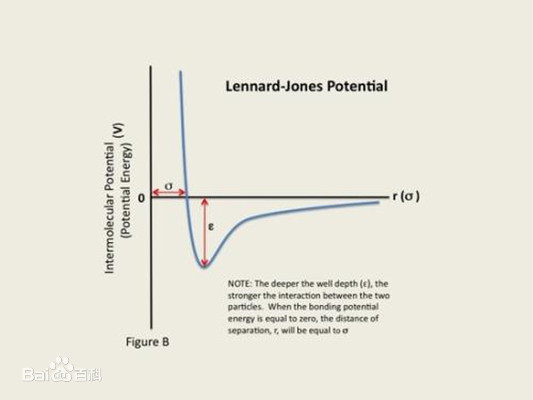
\includegraphics[width=0.45\textwidth]{LJpotential}}  
		实际的相互作用势V(x) 较L-J势更复杂,试求其在平衡位置附近的二阶近似	
	\end{exampleblock}
\end{frame}

\begin{frame}
	\frametitle{}
	\alert{解:} 	不管多复杂,在平衡位置 ($x=a$)附近可泰勒展开
	\begin{equation*}
		V(x)=V(a) +\frac{1}{1!} \frac{\partial V}{\partial x} |_{x=a} (x-a) +\frac{1}{2!} \frac{\partial ^2 V}{\partial x ^2} |_{x=a} (x-a) ^2 + ... 
	\end{equation*}
	一阶导应为零,二阶近似可写为 \\
	$\displaystyle  \begin{array}{lllllllll}
		V(x) &\approx V(a)+\dfrac{1}{2!} \dfrac{\partial ^2 V}{\partial x ^2} |_{x=a} (x-a) ^2   \\
		& =V_0+\dfrac{1}{2} k (x-a) ^2 
	\end{array}$\\
	取坐标原点为($a, V_0 $), 得:\\
	\begin{equation*}
		V(x)=\dfrac{1}{2} k x^2 
	\end{equation*}	
\end{frame}

\begin{frame}
	\frametitle{}
	\begin{block}{弹性势}
		~~\\
		弹簧力正是势函数V(x) 在平衡位置附近的二阶近似\\
		\begin{equation*}
			F=-\frac{ \partial V}{\partial x}=-kx 
		\end{equation*}	
		 把势函数V(x) 改写成弹性势能:\\
		\begin{equation*}
			U(x)=\dfrac{1}{2} \mu \omega ^2 x^2 
		\end{equation*}
	\end{block}	
\end{frame}	

\subsection{量子谐振子方程}

\begin{frame}
	\frametitle{量子谐振子方程}
	\begin{exampleblock} {例2、求解谐振子薛定谔方程}
	\begin{equation*}
		i\hbar \frac{\partial }{\partial t} \Psi (x,t ) =[ -\frac{\hbar^2}{2\mu } \frac{d ^2}{x^2} + \frac{1}{2} \mu \omega ^2 x^2   ] \Psi (x, t ) 
	\end{equation*}
	\end{exampleblock}
	\alert{解:} 	令$\Psi (x,t) =\Psi(x) T(t) $ ,  代回方程\\
	时间和位置分离变量:\\
	时间函数: $T(t)  = \exp(-i E t /\hbar) $ \\
	位置函数满足定态薛定谔方程\\
	\begin{equation*}
		\left [ -\frac{\hbar^2}{2\mu} \frac{\mathrm{d} ^2}{\mathrm{d} x^2} +\frac{1}{2}\mu \omega^2 x^2  \right ]\Psi(x)=E\Psi(x) 
	\end{equation*}	
\end{frame}

\begin{frame}
	\frametitle{}
	整理:\\
	\begin{equation*}
		\frac{1}{\dfrac{\mu\omega}{\hbar}} \frac{\mathrm{d} ^2\Psi}{\mathrm{d} x^2} +	\left ( \frac{2E}{\omega \hbar} -\frac{\mu \omega}{\hbar} x^2 \right )\Psi=0
	\end{equation*}
	令:~~$ \xi =\alpha x$,做自变量伸缩变换 \\
	\begin{equation*}
		\frac{\mathrm{d} \Psi}{\mathrm{d} x} =\frac{\mathrm{d} \Psi}{\mathrm{d} \xi} \frac{\mathrm{d} \xi}{\mathrm{d} x}  = \alpha \frac{\mathrm{d} \Psi}{\mathrm{d} \xi}
	\end{equation*}
	\begin{equation*}
		\frac{\mathrm{d} \Psi ^2 }{\mathrm{d} x ^2} =\frac{\mathrm{d}}{\mathrm{d} x}  ( \alpha \frac{\mathrm{d} \Psi}{\mathrm{d} \xi} ) = \alpha ^2 \frac{\mathrm{d} ^2 \Psi}{\mathrm{d} \xi ^2} 
	\end{equation*}
	代回方程, 得\\
	\begin{equation*}
		\left[ \frac{\hbar ^2 \alpha ^2 }{2\mu} \frac{\mathrm{d}}{\mathrm{d} \xi ^2}  + (E- \frac{\mu \omega ^2 \xi ^2}{2 \alpha ^2}  ) \right] \Psi(\xi) =0
	\end{equation*}	
\end{frame}

\begin{frame}
	\frametitle{}
	同除二阶导数项系数, 得\\
	\begin{equation*}
		\left[ \frac{\mathrm{d}}{\mathrm{d} \xi ^2}  + \frac{2\mu}{\hbar ^2 \alpha ^2 } (E- \frac{\mu \omega ^2 \xi ^2}{2 \alpha ^2}  ) \right] \Psi(\xi) =0
	\end{equation*}
	令 $\dfrac{\mu ^2 \omega ^2 }{\hbar ^2 \alpha ^ 4}=1 $,得伸缩系数:\\
	\begin{equation*}
		\alpha ^2= \frac{\mu\omega}{\hbar}
	\end{equation*}
	引入特征值\\
	\begin{equation*}
		\lambda = \frac{2E}{\omega \hbar}
	\end{equation*}
	得二阶常微分方程\\
	\begin{equation*}
		\left[ \frac{\mathrm{d} ^2\Psi}{\mathrm{d} \xi^2} + \left( \lambda - \xi^2 \right) \right] \Psi=0
	\end{equation*}
\end{frame}

\begin{frame}
	\frametitle{}
	考虑渐近行为, 当 $ |x| \to \infty,  \xi \to \infty$,有 $ \xi ^2  \gg  \lambda $,方程可近似为 \\
	\begin{equation*}
		\left(\frac{\mathrm{d} ^2}{\mathrm{d} \xi^2} - \xi^2 \right) \Psi=0
	\end{equation*}
	方程并无表达式解,但通过检验平方指数函数的导数\\
	\begin{equation*}
		\frac{d^2 }{d \xi ^2} \exp(\frac{\xi ^2}{2}) =(\xi ^2 +1)  \exp(\frac{\xi ^2}{2}) 
	\end{equation*}    
	\begin{equation*}
		\frac{d^2 }{d \xi ^2} \exp( - \frac{\xi ^2}{2}) =(\xi ^2 -1)  \exp( - \frac{\xi ^2}{2}) 
	\end{equation*}     	
\end{frame}

\begin{frame}
	\frametitle{}
	当 $ \xi \to \infty$, 这两导数可近似为:\\
	\begin{equation*}
		(\xi ^2 )  \exp( \frac{\xi ^2}{2}) ~~, ~~ (\xi ^2 )  \exp( - \frac{\xi ^2}{2}) 
	\end{equation*}     
	因此,极限状态解应与如下函数相关联
	\begin{equation*}
		C_1  \exp( \frac{\xi ^2}{2}) + C_2   \exp( - \frac{\xi ^2}{2})  
	\end{equation*}     
	考虑到波函数的有界性,应删除发散项(第一项),得极限状态波函数的简洁形式
	\begin{equation*}
		\Psi_\infty (\xi)  \sim C_2 \exp( - \frac{\xi ^2}{2})  
	\end{equation*}   
\end{frame}

\begin{frame}
	\frametitle{}
	现考虑非极限状态,解函数可写成: 
	\begin{equation*}
		\Psi(\xi) = H(\xi) e^{-\xi^2/2 }  
	\end{equation*}   
	解函数的确定等价于多项式函数 H 的确定。\\
	对上式求导:\\
	\begin{equation*}
		\Psi'(\xi) = H'(\xi) e^{-\xi^2/2 } -  H(\xi) \xi e^{-\xi^2/2 } 
	\end{equation*}  
	\begin{equation*}
		\Psi''(\xi) = \left[  \left( \xi^2 -1 \right) H -2\xi H' +H''  \right] e^{-\xi^2/2}
	\end{equation*}  
	代回原方程  $ \displaystyle \dfrac{\mathrm{d} ^2\Psi}{\mathrm{d} \xi^2} + \left( \lambda - \xi^2 \right) \Psi=0 $  \\ 
\end{frame}

\begin{frame}
	\frametitle{}
	得关于多项式$H(\xi)$的方程: \\  
	\begin{equation*}
		H'' -2 \xi H' +(\lambda -1) H=0 
	\end{equation*}  
	取$\lambda -1= 2n $,方程转化为n阶厄密方程
	\begin{equation*}
		H'' -2 \xi H' +2n H=0 
	\end{equation*}  
	由
	\begin{equation*}
		\lambda = 2n +1 = \frac{2E}{\hbar  \omega}  
	\end{equation*}  
	解出能量固有值(能级)
	\begin{equation*}
		E_n=\left(n+\frac{1}{2}\right) \hbar \omega, ~~~  ( n=0,1,2, ...)  
	\end{equation*}  
	固有函数由n阶厄密方程给出......
\end{frame}

%%%%%%%%%%%%%%%%%%%%%%%%%%%%%%%%%%
\subsection{厄密方程}

\begin{frame}
	\frametitle{厄密方程}
	\begin{exampleblock} {例3、求解n阶厄密方程}
		\begin{equation*}
			H'' -2 \xi H' +2n H=0 
		\end{equation*}  
	\end{exampleblock}
	\alert{解:} 	幂级数方法求解,令:
	\begin{equation*}
		H=\sum_{k=0}^{\infty} c_k \xi ^k
	\end{equation*}     
	求一阶导和二阶导,代回厄密方程,可得系数递推式:
	\begin{equation*}
		c_{k+2} = \frac{ 2(k-n)}{(k+2)(k+1) } c_k, ~~  \left( k=0,1,2,3, ...  \right)
	\end{equation*}   
\end{frame}

\begin{frame}
	\frametitle{}
	分偶数阶和奇数阶写
	\begin{equation*}
		c_{2m} = (-1) ^m \frac{2^mn(n-2)(n-4) ... (n-2m+2)  } {(2m)!} c_0
	\end{equation*}   
	显然有 $ c_{2m} =0~, ~~(2m>n)$
	\begin{equation*}
		c_{k} = (-1) ^m \frac{2^mn !! } {k!} c_0, ~~~(2m=k)
	\end{equation*}   
	\begin{equation*}
		c_{2m+1} = (-1) ^m \frac{2^m (n-1) (n-3)(n-5)...(n-2m+1)  } {(2m+1)!} c_1
	\end{equation*}   
	显然有 $ c_{2m+1} =0~, ~~(2m+1>n)$
	\begin{equation*}
		c_{k} = (-1) ^m \frac{2^m n!! }{k!} c_1, ~~~ (2m+1=k)
	\end{equation*}  
\end{frame}

\begin{frame}
	\frametitle{}
	所有系数求得,幂级数得解\\
	$\displaystyle \begin{cases}
		y_1(\xi)  = [1- \dfrac{2n}{2!} \xi^2+ \dfrac{2^2n(n-2)}{4!} \xi^4 -...  ] \\
		\\
		y_2(\xi)  = [\xi- \dfrac{2(n-1)}{3!} \xi^3+ \dfrac{2^2(n-1)(n-3) }{5!}\xi^5 -...  ]
	\end{cases}$ \\
	n阶厄密方程的解:
	\begin{equation*}
		H(\xi) =c_0y_1(\xi)+c_1 y_2(\xi).
	\end{equation*}   
 	 量子谐振子方程的解:
	\begin{equation*}
		\Psi(\xi) = [c_0y_1(\xi)+c_1 y_2(\xi) ]e^{-\xi^2/2 }  
  	\end{equation*}   
  	根据波函数的有界性性质, H应取多项式 (不能为无穷级数)。当n为偶数时 , $c_1=0$ , 当n为奇数时 , $c_0=0$ 。 待定系数由定解条件给出...
\end{frame}

\begin{frame}
	\frametitle{}
		为了更好地描述,将系数递推式降幂排列,现令最高次项系数为:
	\begin{equation*}
		c_n =2^n
	\end{equation*}  
	系数递推式可写为:
	\begin{equation*}
		c_{k-2} = -\frac{k(k-1) } { 2(n-k+2)}  c_k
	\end{equation*} 
	\begin{equation*}
		c_{n-2} = -\frac{n(n-1) } { 2\times2}  c_n
	\end{equation*} 
	\begin{equation*}
		c_{n-4} = (-1)^2 \frac{n(n-1)(n-2) (n-3) } { 2\times2\times 4}  2^n
	\end{equation*} 
		\begin{equation*}
		c_{n-2m} = (-1)^m \frac{n! } { 2^m (2m) !! (n-2m)!}  2^n =(-1)^m \frac{n! } {  m ! (n-2m)!}  2^{n-2m} 
	\end{equation*} 
\end{frame}

\begin{frame}
	\frametitle{}
	厄密方程的解为厄米多项式:
	\begin{equation*}
		H_n(\xi) =\sum_{m=0}^{M}  (-1)^m \frac{n! } {  m ! (n-2m)!}  2^{n-2m} \xi^{n-2m} ,  ~~~ M=[n/2]
	\end{equation*}   
	量子谐振子的解为
	\begin{equation*}
		\Psi_n(\xi) = N_n \exp(-\frac{\xi ^2}{2}) H_n(\xi) 
	\end{equation*}   
	归一化解:(...)
	\begin{equation*}
		\Psi_n(x) = \left( \frac{\alpha}{\sqrt{\pi} 2^n n!}  \right) ^{1/2}  \exp(-\frac{ \alpha^2 x^2}{2}) H_n( \alpha x) 
	\end{equation*}  
	定态波函数为
	\begin{equation*}
		\Psi_n(x,t) = \left( \frac{\alpha}{\sqrt{\pi} 2^n n!}  \right) ^{1/2}  \exp(-\frac{ \alpha^2 x^2}{2} -\frac{i}{\hbar} E_n t ) H_n( \alpha x) 
	\end{equation*}  	
\end{frame}

\begin{frame}
	\frametitle{作业:}
	1、计算积分\\ 
	$\begin{array}{lllllllll}
		 &\int\limits_{0}^{+\infty} e^{-x^2 /2} dx
	\end{array}$ \\ \vspace{0.6em}
	2、 根据厄米多项式表达式,写出前五个厄米多项式,并分析$H'_n (x)$ 与$H_{n-1} (x)$  之间的联系\\ \vspace{0.6em}
	3、 求解厄米方程\\ \vspace{0.6em}
	$\begin{array}{lllllllll}
		& \dfrac{d^2 H}{d x^2} -2x \dfrac{d y}{d x} +4n H =0 		
	\end{array}$ \\ \vspace{0.6em}
	4、  列出厄米方程的几种形式,说明厄米方程的特点
\end{frame}

%%%%%%%%%%%%%%%%%%%%%%%%%%%%%%%%%%%%%%%%%%%%%
\section{4.厄密多项式及性质}

\subsection{生成函数}

\begin{frame}
	\frametitle{ 生成函数 }
	\begin{exampleblock} { 例1、求厄密多项式的生成函数 }
		找一个函数,它的展开系数刚好就是Hermite 多项式
		 \begin{equation*}
			w(x,t)=e^{2xt-t^2}
		\end{equation*}
		试证明,上述二元函数就是Hermite多项式的一个母函数
	\end{exampleblock}
	\alert {解:}	把函数做关于变量t的Taylor 展开:
	\begin{equation*}
		w(x,t) =\sum_{n=0}^{\infty} \frac{1}{n!}  c_n(x) t^n
	\end{equation*}
	需证明:
	\begin{equation*}
		\left[  \frac{d^2}{dx^2} -2x\frac{d}{dx} +2n  \right] c_n(x)=0
	\end{equation*}
\end{frame}

\begin{frame}
	\frametitle{  }
	\textbf{证明:}	1)、由 $  \dfrac{\partial w}{\partial x} =2t e^{2xt-t^2} =2t ~w(x,t) $, 得 \\ 
	$ \sum\limits_{n=0}^{\infty} \dfrac{1}{n!}  c~'_n(x) t^n  = 2t  \sum\limits_{n=0}^{\infty} \dfrac{1}{n!}  c_n(x) t^n $ \\
	\hspace{2.3cm}	$=  \sum\limits_{n=0}^{\infty} \dfrac{1}{n!}  2c_{n}(x) t^{n+1} $\\
	\hspace{2.3cm}	$=  \sum\limits_{n=1}^{\infty} \dfrac{1}{n!}  2nc_{n-1}(x) t^{n}   $ \\
	比较系数,有:\\
	\hspace{2.1cm}	{ $c~'_n(x)=2nc_{n-1}(x)$} \\  \vspace{0.3cm}
	\hspace{2.1cm}	$c~''_n(x)=2nc~'_{n-1}(x)=4n(n-1)c_{n-2}(x)$ \\  	
\end{frame}

\begin{frame}
	\frametitle{  }
	2)由 $  \dfrac{\partial w}{\partial t} =2(x-t) e^{2xt-t^2} =2(x-t) ~w(x,t) $, 得 \\ 
	\hspace{2.1cm}		$  \dfrac{\partial w}{\partial t} +2(t-x) ~w(x,t) =0$ \\ 
	把展开式代入上式\\ 
	{$  \sum\limits_{n=1}^{\infty} \dfrac{1}{n!}n c_n(x) t^{n-1} +\sum\limits_{n=0}^{\infty} \dfrac{1}{n!}2(t-x) c_n(x)t^n=0$ } \\ \vspace{0.3cm}
	{$ \sum\limits_{n=1}^{\infty} \dfrac{1}{n!}n c_n(x) t^{n-1} +\sum\limits_{n=0}^{\infty} \dfrac{-2x}{n!} c_n(x)t^n +\sum\limits_{n=0}^{\infty}\dfrac{2}{n!} c_n(x)t^{n+1}=0$ } \\ \vspace{0.3cm}
	{$ \sum\limits_{n=0}^{\infty} \dfrac{1}{n!} c_{n+1}(x) t^{n} +\sum\limits_{n=0}^{\infty} \dfrac{-2x}{n!} c_n(x)t^n +\sum\limits_{n=1}^{\infty}\dfrac{2n}{n!} c_{n-1}(x)t^n=0$ } 
\end{frame}

\begin{frame}
	\frametitle{  }
	比较系数,有:\\
	\hspace{2.1cm}	{  $ c_{n+1}(x) -2xc_n(x) +2nc_{n-1} (x) =0 $} \\ \vspace{0.3cm}
	\hspace{2.1cm}	{  $ c_{n}(x) -2xc_{n-1}(x) +2(n-1)c_{n-2} (x) =0 $} \\ 
	3) 把(1)中得到的结论 \\
	\hspace{2.1cm}	{ $c~'_n(x)=2nc_{n-1}(x)$} \\  \vspace{0.3cm}
	\hspace{2.1cm}	$c~''_n(x)=4n(n-1)c_{n-2}(x)$ \\  
	代入(2)中得到的结论,得:\\
	\hspace{2.1cm} $  c_{n}(x) - \dfrac{x}{n}c~'_{n}(x) +\dfrac{1}{2n}c~''_{n} (x) =0 $ \\
	整理为:
	\begin{equation*}
 	    \left[  \dfrac{d^2}{dx^2} -2x\frac{d}{dx} +2n  \right] c_n(x)=0 
	\end{equation*}
 	\textcolor{red}{证毕!}\\
	即有: $c_n(x)=H_n(x)  $ 
\end{frame}

\subsection{性质}
\begin{frame}
	\frametitle{递推公式 }
	{  既然: $c_n(x)=H_n(x) $}  \\ \vspace{0.3cm}
	\hspace{1cm} 	{  $c~'_n(x)=2nc_{n-1}(x)    $ }   \\ 
	{  $ ~\to~~  H~'_n(x)=2nH_{n-1}(x)    $}   \\ \vspace{0.3cm}
	\hspace{1cm} 	{  $ c_{n}(x) -2xc_{n-1}(x) +2(n-1)c_{n-2} (x) =0  $ }   \\ 
	{  $~\to~~   H_{n}(x) -2xH_{n-1}(x) +2(n-1)H_{n-2} (x) =0  $ } \\ \vspace{0.3cm}
	有: $H_0(x)=1,  H_1(x)=2x, $	
\end{frame}

\begin{frame}
	\frametitle{ 微分形式 }
	$ \displaystyle w(x,t) =\sum_{n=0}^{\infty} \frac{1}{n!}  c_n(x) t^n $, ~~~~
	{ $ \displaystyle w(x,t) =\sum_{n=0}^{\infty} \frac{1}{n!}  H_n(x) t^n  $} \\
	由Taylor展式,知:\\
	{ $ \displaystyle  H_n(x) = \left[  \frac{\partial ~^n w  }{\partial t^n}  \right] _{t=0} $}\\ 
	\hspace{1cm} {$ 	\displaystyle  =e^{x^2}   \left[  \frac{\partial ^n }{\partial t^n}  e^{-(x-t)^2}   \right] _{t=0}   $}  \\ 
	\hspace{1cm} {$ 	\displaystyle  =(-1) ^n e^{x^2}   \left[  \frac{d~^n }{d~u^n}  e^{-u^2}   \right] _{u=x}   $}  \\ 
	{$ 	\displaystyle H_n(x) =(-1) ^n e^{x^2}  \frac{d~^n }{d~x^n}  e^{-x^2}   $}  \\ 
\end{frame}

\begin{frame}
	\frametitle{ 正交性 }
	\begin{exampleblock} { 例2、证明厄密多项式正交性 }
	是带权函数($\rho(x) =exp(-x^2)$)的正交函数系:\\
	{$ \displaystyle  
	\left\{  
	\begin{array}{ccccc}
		\int\limits_{-\infty}^{+\infty} e^{-\xi^{2}} H_m(\xi) H_n(\xi)d\xi &=&0 ~~~~~~\\
		\int\limits_{-\infty}^{+\infty} e^{-\xi^{2}} H_n(\xi) H_n(\xi)d\xi &=&2^n n! \sqrt{\pi}  
	\end{array}
	\right.  
	$} 
	\end{exampleblock}
\alert {证明:}	
	谐振子方程:{ $ \displaystyle \dfrac{\mathrm{d} ^2\Psi}{\mathrm{d} \xi^2} + \left( \lambda - \xi^2 \right) \Psi=0  $  }  \\
	代入$\lambda=2n+1 $~\\
	$\to   \Psi''_n +(2n+1-\xi^2) \Psi_n =0$ \\
	解为: $u_n(x)=H_n(\xi) e^{-\xi^{2}/2}$ , 代回方程,得:
\end{frame}

\begin{frame}
	\frametitle{  }
	$u''_n+ (2n+1-\xi^2) u_n =0    ~, ~u''_m+ (2m+1-\xi^2) u_m =0  $\\  \vspace{0.3cm}
	$u_mu''_n +(2n+1-\xi^2) u_mu_n =0 $\\ 
	$u_nu''_m+ (2n+1-\xi^2) u_nu_m =0  $  \\  \vspace{0.3cm}
	$u_mu''_n -u_nu''_m +2(n-m)u_nu_m=0 $\\  \vspace{0.3cm}
	$ \int\limits_{-\infty}^{+\infty} [u_mu''_n -u_nu''_m] d\xi  $\\
	\hspace{2cm} 	$= [u_mu''_n -u_nu''_m] \left |_{-\infty} ^{+\infty}  \right. -\int\limits_{-\infty}^{+\infty} [u'_mu'_n -u'_nu'_m] d\xi =0$\\   
	因此	$ 2(n-m) \int\limits_{-\infty}^{+\infty} u_nu_m d\xi =0$ \\   \vspace{0.3cm}
	即:{ $ \int\limits_{-\infty}^{+\infty} e^{-\xi^{2}} H_m(\xi) H_n(\xi)d\xi =0 $ }	
\end{frame}

\begin{frame}
	\frametitle{  }
	由递推公式:\\
	{$H_{n} -2xH_{n-1} +2(n-1)H_{n-2} =0  $ } \\
	=> 	{ $H^2_{n}-2xH_n H_{n-1}+2(n-1) H_n H_{n-2} =0  $ }\\   \vspace{0.3cm}
	{$H_{n+1} -2xH_{n} +2nH_{n-1} =0  $ } \\
	=>   { $H_{n+1} H_{n-1}-2xH_{n} H_{n-1}+2nH^2_{n-1} =0  $ } \\  \vspace{0.3cm}
	两次相减\\
     $H^2 _n(\xi) -H_{n+1} H_{n-1}=2n H^2 _{n-1}(\xi) - 2(n-1) H_n H_{n-2}$ \\	  \vspace{0.3cm}
	乘以权重函数再积分,  得积分递推式:\\
	{$\int\limits_{-\infty}^{+\infty} e^{-\xi^2} H^2 _n(\xi) d\xi =2n \int\limits_{-\infty}^{+\infty} e^{-\xi^{2}} H^2 _{n-1}(\xi) d\xi$ }\\	
\end{frame}	

\begin{frame}
	\frametitle{  }
	{$\int\limits_{-\infty}^{+\infty} e^{-\xi^2} H^2 _n(\xi) d\xi =2n \int\limits_{-\infty}^{+\infty} e^{-\xi^{2}} H^2 _{n-1}(\xi) d\xi$ }\\
	$= 2n \times 2(n-1) \int\limits_{-\infty}^{+\infty} e^{-\xi^{2}} H^2 _{n-2}(\xi) d\xi$  \\
	$= 2n \times 2(n-1) ... (2(n-n)) \int\limits_{-\infty}^{+\infty} e^{-\xi^{2}} H^2 _{0}(\xi) d\xi$  \\
	$= 2^n n! \int\limits_{-\infty}^{+\infty} e^{-\xi^{2}} H^2 _{0}(\xi) d\xi$  \\	
	$= 2^n n! \int\limits_{-\infty}^{+\infty} e^{-\xi^{2}} d\xi$  \\	
	$= 2^n n! \sqrt{\pi} $ \\	
\end{frame}	

\subsection{归一化系数}

\begin{frame}
	\frametitle{求归一化系数}
	固有解为
	\begin{equation*}
		\Psi_n(\xi) = N_n \exp(-\frac{\xi ^2}{2}) H(\xi) 
	\end{equation*}   
	\begin{equation*}
		\int\limits_{-\infty}^{+\infty} [N_n \exp(-\frac{\xi ^2}{2}) H(\xi) ]^2d\xi  =N^2 _n 2^n n! \sqrt{\pi}=1
	\end{equation*}  
	\begin{equation*}
    	N_n=\dfrac{1}{(2^n n! \sqrt{\pi}) ^{1/2}}
	\end{equation*}    
\end{frame}	

\begin{frame}
	\frametitle{  }
	归一化固有函数:\\  
	{ $  \displaystyle  \Psi_n(x) =  \left(  \dfrac{\alpha}{\sqrt{\pi} 2^n n! } \right) ^{1/2} e^{-a^2 x^2}  H_n(\alpha x)  $ } \\ 
	定态波函数: \\
	{ $  \displaystyle  \Psi_n(x,t) =  \Psi_n(x) e^{-\dfrac{i}{\hbar} E_n t } $} \\
	{$  \displaystyle = \left(  \dfrac{\alpha }{\sqrt{\pi} 2^n n! } \right) ^{1/2} e^{-a^2 x^2 -\dfrac{i}{\hbar} E_n t }  H_n(\alpha  x)  $ } \\  
	叠加解:\\
	{\large $  \displaystyle \Psi(x,t) =\sum a_n \Psi_n(x,t)  $} \\	
\end{frame}	

\begin{frame}
	\frametitle{  }
	下图给出了基态和第一激发态函数及概率分布\\
	%\usetikzlibrary {datavisualization.formats.functions} 
	\begin{tikzpicture}[baseline, scale=.7]
	\datavisualization [ scientific axes, 
		visualize as smooth line/.list={sin,cos}, style sheet=strong colors,
		style sheet=vary dashing,
		sin={label in legend={text=$\Psi_0(x)$}}, 
		cos={label in legend={text=$\Psi_1(x) $}}, 
		data/format=function ]
		data [set=sin] {
			var x : interval [-3:3];
			func y = 1/sqrt(sqrt(pi))* exp(-0.5 * \value x * \value x  )  ;
		}
		data [set=cos] {
			var x : interval [-3:3];
			func y = 2*\value x /sqrt(2*sqrt(pi))* exp(-0.5 * \value x * \value x  )  ;
		};
	\end{tikzpicture}	
   %\usetikzlibrary {datavisualization.formats.functions} 
   	\begin{tikzpicture}[baseline, scale=.7]
   	\datavisualization [ scientific axes, 
   		visualize as smooth line/.list={sin,cos}, style sheet=strong colors,
   		style sheet=vary dashing,
   		sin={label in legend={text=$|\Psi_0(x)|^2$}}, 
   		cos={label in legend={text=$|\Psi_1(x)|^2$}}, 
   		data/format=function ]
   		data [set=sin] {
   			var x : interval [-3:3];
   			func y = 1/sqrt(pi)* exp(- \value x * \value x  )  ;
   		}
   		data [set=cos] {
   		var x : interval [-3:3];
   		func y = 2*\value x * \value x /sqrt(pi)* exp(- \value x * \value x  )  ;
   		};
   \end{tikzpicture}
\end{frame}	

\begin{frame}
	\frametitle{ 课堂测试! }	
	\begin{exampleblock} {课堂测试题1:}
		求处于如下势场:
		\begin{equation*}
			V(x)= \frac{1}{2} \mu \omega ^2 x^2  +\mu
		\end{equation*}
		中粒子的能量固有值和定态波函数。
	\end{exampleblock}	
\end{frame}	

\begin{frame}
	\frametitle{ 作业 }
	1、将函数$f(x)=x^3+2x^2 +1$ 按厄米多项式展开\\ 
	参考答案:$f(x) =\dfrac{1}{8} H_3 + \dfrac{1}{2} H_2 +\dfrac{3}{4} H_1 + 2 H_0 $\\
	2、写出厄米多项式的递推公式,并求 $H_n(0) ,   H'_n(0) , H_n(1) ,   H'_n(1)  $\\ 
	3、求解如下初值问题\\
	\begin{equation*}
		\left\{ 
		\begin{aligned}
			& i \hbar \dfrac{\partial \Psi}{\partial t}  = \left[  -\dfrac{\hbar ^2}{2\mu} \dfrac{\partial ^2}{\partial x^2} +\dfrac{1}{2}  \mu \omega ^2 x ^2 \right] \Psi \\
			& \Psi(x, 0) =\psi(x)
		\end{aligned} 
		\right.
	\end{equation*}
\end{frame}	

\begin{frame}
	\frametitle{ 作业 }
	4、	电荷为q的谐振子,受到沿 x 方向的外电场$\xi $的作用时,其势场为:
	\begin{equation*}
		V(x)= \frac{1}{2} \mu \omega ^2 x^2  +q\xi x  
	\end{equation*}
	求解其能量固有值和定态波函数。(移轴法)
\end{frame}

\begin{frame}
	\frametitle{课外读物和思考}
	薛定谔方程的数值解法:\\
	Matlab or Python or VASP
\end{frame}	
%%%%%%%%%%%%%%%%%%%%%%%%%%%%%%%%%%%%%%%%%%%%%%
%%%%%%%%%%%%%%%%%%%%%%%%%%%%%%%%%%%%%%%%%%%%%%%%%
\begin{frame}
		\frametitle{}
		\Background[1] 
	    \begin{center}
		{ {\Huge 第四章~~氢原子~~  (6学时)}}
	    \end{center}    
\end{frame}
%%%%%%%%%%%%%%%%%%%%%%%%%%%%%%%%%%%%%%%%%%%%%xs

\section{1.氢原子薛定谔方程分离变量 }

\subsection{相对坐标系}

\begin{frame}
	\frametitle{氢原子薛定谔方程}
	氢原子含一原子核和一核外电子,是二体问题。\\
	{\Bullet}哈密顿量为:
	\begin{equation*}
		H=\left[-\frac{\hbar^2}{2 m_1} \nabla_1 ^2 + V(\vec{r_1},t) \right]  + \left[-\frac{\hbar^2}{2 m_2} \nabla_2 ^2 + V(\vec{r_2},t) \right]  +U(| \vec{r_1}-\vec{r_2} | )
	\end{equation*}
	其中 V为背景势,U为库仑势(相互作用势):
	\begin{equation*}
		U(| \vec{r_1}-\vec{r_2} | )=-\frac{e_s ^2}{| \vec{r_1}-\vec{r_2} |} ~~,~~~ e_s =\frac{Ze}{\sqrt{4\pi\epsilon_0}}
	\end{equation*}
\end{frame}

\begin{frame}
	\frametitle{}
	{\Bullet}薛定谔方程为:
	\begin{equation*}
		i\hbar \frac{\partial }{\partial t} \Psi (\vec{r_1},\vec{r_2},t ) =H (\vec{r_1},\vec{r_2}, t  )  \Psi (\vec{r_1},\vec{r_2},t ) 
	\end{equation*}
	{\Bullet}当背景势V不显含时间t,时空可分离变量。解得的时间函数为:
	\begin{equation*}
		f(t) =e^{-iEt/\hbar}
	\end{equation*}
	空间函数服从定态薛定谔方程:
	\begin{equation*}
		\left[-\frac{\hbar^2}{2 m_1} \nabla_1 ^2 + V_1  -\frac{\hbar^2}{2 m_2} \nabla_2 ^2 + V_2  +U_{1,2} \right] \Psi (\vec{r_1},\vec{r_2}) =E \Psi (\vec{r_1},\vec{r_2}) 
	\end{equation*}
\end{frame}		

\begin{frame}
	\frametitle{}
	对于自由氢原子,背景势V=0,方程简化为:
	\begin{equation*}
		\left[-\frac{\hbar^2}{2 m_1} \nabla_1 ^2  -\frac{\hbar^2}{2 m_2} \nabla_2 ^2 +U(| \vec{r_1}-\vec{r_2} | ) \right] \Psi (\vec{r_1},\vec{r_2}) =E \Psi (\vec{r_1},\vec{r_2}) 
	\end{equation*}
	其中, 
	\begin{equation*}
		U(| \vec{r_1}-\vec{r_2} | )=-\frac{e_s ^2}{| \vec{r_1}-\vec{r_2} |} 
	\end{equation*}
	这是一个6维势,决定着方程求解的难度.
\end{frame}		

\begin{frame}
	\frametitle{相对坐标}
	{\Bullet} 引入相对坐标和质心坐标\\ \vspace{0.6em}
	令:(1)
	$\displaystyle \begin{cases}
		\vec{r} (x,y,z)= \vec{r_1}-\vec{r_2}  , \qquad \text{(相对坐标)} \\ \vspace{0.3em}
		\vec{R} (X,Y,Z)= \dfrac{ m_1\vec{r_1}+ m_2\vec{r_2}  }{ m_1+m_2} , \qquad \text{(质心坐标)} 
	\end{cases}$ \\	
	\hspace{1.6em} (2)
	$\displaystyle \begin{cases}
		m = \dfrac{m_1m_2}{m_1+m_2}, \qquad \text{(折合质量)}\\
		M= m_1+m_2,  \qquad \text{(质心质量)}
	\end{cases}$ \\	\vspace{1em}
	可实现变量分离!
\end{frame}		

\begin{frame}
	有坐标函数:
	$\displaystyle \begin{cases}
		\vec{r_1}= f_1(\vec{r},\vec{R}) \\
		\vec{r_2}= f_2(\vec{r},\vec{R}) 
	\end{cases}$ \\	
	对其求导:
	\begin{equation*}
		\begin{split}
		\dfrac{d}{dx_1}= &\dfrac{\partial}{\partial X}  \dfrac{\partial X}{ \partial x_1} +\dfrac{\partial }{\partial x}  \dfrac{\partial x}{\partial x_1} 
		= \dfrac{m_1}{M}  \dfrac{\partial }{ \partial X} +\dfrac{\partial }{\partial x} \\ \vspace{0.3em}
		\dfrac{d^2}{dx^2 _1}= &\dfrac{m^2 _1}{M^2 }  \dfrac{\partial^2 }{ \partial X^2} + \dfrac{2m _1}{M }  \dfrac{\partial^2 }{ \partial X \partial x}+\dfrac{\partial ^2 }{\partial x^2} \\		
		\nabla ^2 _1= &\dfrac{m^2 _1}{M^2 }  \nabla ^2 _R + \dfrac{2m _1}{M }  (\dfrac{\partial^2 }{ \partial X \partial x} +  \dfrac{\partial^2 }{ \partial Y \partial y} + \dfrac{\partial^2 }{ \partial Z \partial z})    + \nabla ^2 _r  \\
		\nabla ^2 _2= &\dfrac{m^2 _2}{M^2 }  \nabla ^2 _R - \dfrac{2m _2}{M }  (\dfrac{\partial^2 }{ \partial X \partial x} +  \dfrac{\partial^2 }{ \partial Y \partial y} + \dfrac{\partial^2 }{ \partial Z \partial z})    + \nabla ^2 _r
		\end{split}
	\end{equation*}
\end{frame}		

\begin{frame}
	结合在一起,得:	
	\begin{equation*}
		\dfrac{1}{m_1}\nabla ^2 _1	+ \dfrac{1}{m_2}\nabla ^2 _2 = \dfrac{1}{M}\nabla ^2 _R+ \dfrac{1}{m}\nabla ^2 _r
	\end{equation*}	
	代回简化后的方程,得:
	\begin{equation*}
		\left[-\frac{\hbar^2}{2 M} \nabla_R ^2  -\frac{\hbar^2}{2 m} \nabla_r ^2 +U(\vec{r} ) \right] \Psi (\vec{R},\vec{r}) =E \Psi (\vec{R},\vec{r}) 
	\end{equation*}
	相对和质心坐标可分离变量! \\ 
	令: $\Psi (\vec{R},\vec{r}) = \psi (\vec{R}) \Psi (\vec{r})  $, 代入上方程,
\end{frame}		

\begin{frame}
	\frametitle{质心运动方程}
	得方程(1):
	\begin{equation*}
		-\frac{\hbar^2}{2 M} \nabla_R ^2  \psi (\vec{R}) =E_c \psi (\vec{R})  ..... (1)
	\end{equation*}	
	这是质心运动方程,解为自由粒子平面波:
	\begin{equation*}
	\psi (\vec{R},t)=-\frac{1}{(2\pi\hbar)^{3/2}}e^{-\frac{i}{\hbar}(E_c t -\vec{p}\cdot\vec{R})}
	\end{equation*}
\end{frame}		

\begin{frame}
	\frametitle{相对运动方程}
	不失一般性,方程(2)写为:
	\begin{equation*}
		\left[-\frac{\hbar^2}{2 m} \nabla ^2 +U(\vec{r}) \right] \Psi (\vec{r}) =E \Psi (\vec{r})   ..... (2)
	\end{equation*}
	这是相对运动方程,是核与核外电子相对于质心的运动方程.\\
	可以近似地看成是核外电子相对于核的运动方程.
\end{frame}	

\begin{frame}
	其中,
	\begin{equation*}
		U(\vec{r})=U(| \vec{r_1}-\vec{r_2} | )=-\frac{e_s ^2}{| \vec{r_1}-\vec{r_2} |} = -\frac{e_s ^2}{r} ~~,~~~ r =\sqrt{x^2+y^2+z^2}
	\end{equation*}
	 有
	\begin{equation*}
		U(r)=-\frac{e_s ^2}{r}
	\end{equation*}	
	是一个与角量无关的物理量。 \\
	若改用球坐标系描述方程(2), 则经向r可分离变量!\\
	\begin{equation*}
		\left[-\frac{\hbar^2}{2 \mu} \nabla ^2 +U(r) \right] \Psi (\vec{r}) =E \Psi (\vec{r})   ..... (2)
	\end{equation*}
	因此要求普拉斯算子$\nabla ^2$的球坐标系形式
\end{frame}		

\subsection{球坐标拉普拉斯}

\begin{frame}
	\frametitle{球坐标拉普拉斯算子}
	\例[1.已知x,y,z)坐标系下的拉普拉斯算子为] 
	{\begin{equation*}
		\nabla ^{2}  = \dfrac{\partial ^2}{\partial x^2} +\dfrac{\partial^2 }{\partial y^2} +\dfrac{\partial^2  }{\partial z^2}
	\end{equation*}\\
	求 ($r, \theta, \varphi $)坐标系下的拉普拉斯算子 \\ 
	}
	\begin{center}
		   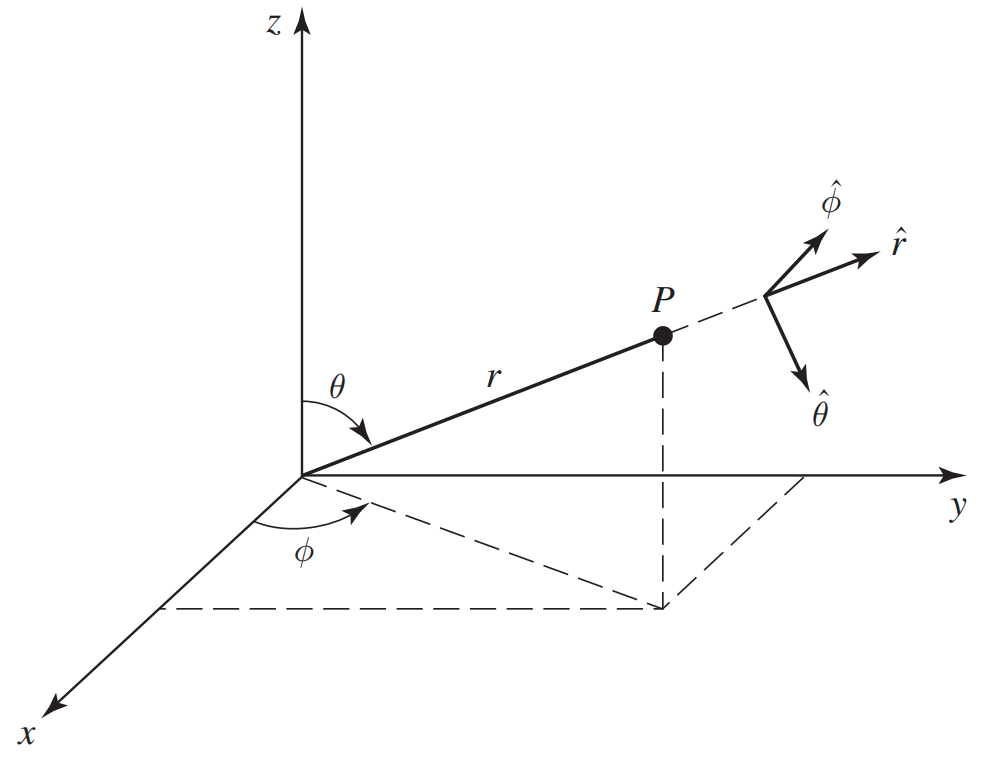
\includegraphics[width=0.48\textwidth]{figs/2022-03-28-22-51-18.png}
	\end{center}
\end{frame}

\begin{frame}
	  \frametitle{}	  
	\alert{解:}  坐标变换关系为:\\
	$\begin{cases}
		x= r\sin \theta \cos \varphi \\
		y= r\sin \theta \sin \varphi \\
		z=r\cos \theta
	\end{cases} $ \\
	对函数$u(x,y,z)$,进行 $r, \theta, \varphi $求导,有:\\ \vspace{0.6em}
	{\small $\begin{cases}
		\dfrac{\partial {u}}{\partial {r}}=\dfrac{\partial {u}}{\partial x} \dfrac{\partial {x}}{\partial {r}}+\dfrac{\partial u}{\partial {y}} \dfrac{\partial {y}}{\partial {r}}+\dfrac{\partial u}{\partial z} \dfrac{\partial z}{\partial {r}} \\ \vspace{0.3em}
		\dfrac{\partial {u}}{\partial \theta}=\dfrac{\partial {u}}{\partial x} \dfrac{\partial{x}}{\partial \theta}+\dfrac{\partial u}{\partial {y}} \dfrac{\partial {y}}{\partial \theta}+\dfrac{\partial{u}}{\partial z} \dfrac{\partial z}{\partial \theta} \\ \vspace{0.3em}
		\dfrac{\partial {u}}{\partial \varphi}=\dfrac{\partial u}{\partial x} \dfrac{\partial{x}}{\partial \varphi}+\dfrac{\partial u}{\partial y} \dfrac{\partial y}{\partial \varphi}+\dfrac{\partial u}{\partial z} \dfrac{\partial z}{\partial \varphi}
	\end{cases} $}\\ \vspace{1em}
\end{frame}	

\begin{frame}
	写成矩阵形式 \\ \vspace{1em}
	{\small $\left[\begin{array}{ccc}
		\dfrac{\partial u}{\partial r} \\ \vspace{0.3em}
		\dfrac{\partial u}{\partial \theta} \\ \vspace{0.3em}
		\dfrac{\partial u}{\partial \varphi}
	\end{array}\right]$
	=
	$\left[\begin{array}{ccc}
		\sin \theta \cos \varphi & \sin \theta \sin \varphi & \cos \theta \\ \vspace{0.3em}
		r \cos \theta \cos \varphi & r \cos \theta \sin \varphi & -r \sin \theta \\ \vspace{0.3em}
		-r \sin \theta \sin \varphi & r \sin \theta \cos \varphi & 0
	\end{array}\right]$
	$\left[\begin{array}{ccc}
		\dfrac{\partial u}{\partial x} \\ \vspace{0.3em}
		\dfrac{\partial u}{\partial y} \\ \vspace{0.3em}
		\dfrac{\partial u}{\partial z}
	\end{array}\right]$
	}\\
	{\small $\left[\begin{array}{ccc}
		\dfrac{\partial u}{\partial r} \\ \vspace{0.3em}
		\dfrac{\partial u}{\partial \theta} \\ \vspace{0.3em}
		\dfrac{\partial u}{\partial \varphi}
	\end{array}\right]$
	=
	$\left[\begin{array}{ccc}
		1 & 0 & 0 \\ \vspace{0.3em}
		0 & r  & 0 \\ \vspace{0.3em}
		0 & 0 & r \sin \theta 
	\end{array}\right]$
	$\left[\begin{array}{ccc}
		\sin \theta \cos \varphi & \sin \theta \sin \varphi & \cos \theta \\ \vspace{0.3em}
		\cos \theta \cos \varphi & \cos \theta \sin \varphi & - \sin \theta \\ \vspace{0.3em}
		-\sin \varphi &  \cos \varphi & 0
	\end{array}\right]$
	$\left[\begin{array}{ccc}
		\dfrac{\partial u}{\partial x} \\ \vspace{0.3em}
		\dfrac{\partial u}{\partial y} \\ \vspace{0.3em}
		\dfrac{\partial u}{\partial z}
	\end{array}\right]$
	}
\end{frame}	

\begin{frame}
	\small {$
		\left[\begin{array}{ccc}
			\dfrac{\partial u}{\partial x} \\
			\dfrac{\partial u}{\partial y} \\
			\dfrac{\partial u}{\partial z}
		\end{array}\right]$
		=
		$\left[\begin{array}{ccc}
			\sin \theta \cos \varphi & \cos \theta \cos \varphi & -\sin \varphi \\
			\sin \theta \sin \varphi &  \cos \theta \sin \varphi &  \cos \varphi \\
			\cos \theta & -\sin \theta & 0
		\end{array}\right]$
		$\left[\begin{array}{ccc}
			\dfrac{\partial u}{\partial r} \\
			\dfrac{1}{r}\dfrac{\partial u}{\partial \theta} \\
			\dfrac{1}{r \sin \theta}\dfrac{\partial u}{\partial \varphi}
		\end{array}\right]
		$}	\\ \vspace{0.3cm}
	\small {$
		\left[\begin{array}{ccc}
			\dfrac{\partial u}{\partial x} \\
			\dfrac{\partial u}{\partial y} \\
			\dfrac{\partial u}{\partial z}
		\end{array}\right]$
		=
		$\left[\begin{array}{ccc}
			{\vec{e}_r}&  {\vec{e}_\theta} & {\vec{e}_\varphi}
		\end{array}\right]$
		$\left[\begin{array}{ccc}
			\dfrac{\partial u}{\partial r} \\
			\dfrac{1}{r}\dfrac{\partial u}{\partial \theta} \\
			\dfrac{1}{r \sin \theta}\dfrac{\partial u}{\partial \varphi}
		\end{array}\right]
		$}	\\ 
\end{frame}	

\begin{frame}
	球坐标系下, 有:
	\begin{equation*}
	\nabla=\vec{e}_{r} \frac{\partial}{\partial r}+\frac{1}{r} \vec{e}_{\theta} \frac{\partial}{\partial \theta}+\frac{1}{r \sin \theta} \vec{e}_{\varphi} \frac{\partial}{\partial \varphi}
	\end{equation*}
	\begin{equation*}
	\begin{split}
		\nabla ^2&=\nabla \cdot \nabla \\
		&=(\vec{e}_{r} \frac{\partial}{\partial r}+\frac{1}{r} \vec{e}_{\theta} \frac{\partial}{\partial \theta}+\frac{1}{r \sin \theta} \vec{e}_{\varphi} \frac{\partial}{\partial \varphi})  \cdot (\vec{e}_{r} \frac{\partial}{\partial r}+\frac{1}{r} \vec{e}_{\theta} \frac{\partial}{\partial \theta}+\frac{1}{r \sin \theta} \vec{e}_{\varphi} \frac{\partial}{\partial \varphi}) \\
		&=\frac{\partial ^2}{\partial r^2} + ( \frac{1}{r} \frac{\partial}{\partial r} + \frac{1}{r^2} \frac{\partial^2} {\partial \theta ^2}  ) + (\frac{1}{r} \frac{\partial}{\partial r}  + \frac{\cos \theta}{r^2 \sin \theta} \frac{\partial} {\partial \theta }  + \frac{1}{r^2 \sin^2 \theta  } \frac{\partial^2}{\partial\varphi ^2} )\\
		&=\frac{1}{r^2} \frac{\partial }{\partial r} (r^2\frac{\partial }{\partial r} )+
		\frac{1}{r^2 \sin \theta  } \frac{\partial }{\partial \theta } (\sin \theta \frac{\partial }{\partial \theta } )
		+\frac{1}{r^2 \sin^2 \theta  } \frac{\partial^2}{\partial\varphi ^2}
	\end{split}
	\end{equation*}

	{\Bullet}~利用球坐标单位矢(1)正交归一性和(2)微分性质完成计算(见讲义 15页)
\end{frame}	

\begin{frame}
	直角坐标~ $(x,y,z) $: 
	\begin{equation*}
		\nabla ^{2}  = \dfrac{\partial ^2}{\partial x^2} +\dfrac{\partial^2 }{\partial y^2} +\dfrac{\partial^2  }{\partial z^2}
	\end{equation*}
	球坐标~ $(r,\theta, \varphi )$ :
	\begin{equation*}
		\nabla ^{2} =\frac{1}{r^2} \frac{\partial }{\partial r} (r^2\frac{\partial }{\partial r} )+
		\frac{1}{r^2 \sin \theta  } \frac{\partial }{\partial \theta } (\sin \theta \frac{\partial }{\partial \theta } )
		+\frac{1}{r^2 \sin^2 \theta  } \frac{\partial^2}{\partial\varphi ^2}
	\end{equation*}	
	令角向部分为:
	\begin{equation*}
		L^2 = - \left[ \frac{1}{ \sin \theta  } \frac{\partial }{\partial \theta } (\sin \theta \frac{\partial }{\partial \theta } )
		+\frac{1}{ \sin^2 \theta  } \frac{\partial^2}{\partial\varphi ^2} \right]
	\end{equation*}	
	有 :
	\begin{equation*}
		\nabla ^{2} =\frac{1}{r^2} \frac{\partial }{\partial r} (r^2\frac{\partial }{\partial r} )-
		\frac{1}{r^2 } L^2 
	\end{equation*}	
	的确它由径向和角向二部分加和构成,因此可实现径向和角向的分离变量!
\end{frame}	

\begin{frame}
	\frametitle{角向与角动量的关系}	
	角向(方)算子:
	\begin{equation*}
		L^2 = - \left[ \frac{1}{ \sin \theta  } \frac{\partial }{\partial \theta } (\sin \theta \frac{\partial }{\partial \theta } )
		+\frac{1}{ \sin^2 \theta  } \frac{\partial^2}{\partial\varphi ^2} \right]
	\end{equation*}	
    角动量(方)算子:
		\begin{equation*}
		L^2 = -\hbar ^2 \left[ \frac{1}{ \sin \theta  } \frac{\partial }{\partial \theta } (\sin \theta \frac{\partial }{\partial \theta } )
		+\frac{1}{ \sin^2 \theta  } \frac{\partial^2}{\partial\varphi ^2} \right]
	\end{equation*}	
	动量的切向分量
	\begin{equation*}
	p_ \perp  ^2 =  \frac{L^2}{r^2}
	\end{equation*}	
	动量的径向分量
	\[ p_r ^2 = -\hbar ^2  \frac{1}{r^2} \frac{\partial }{\partial r} (r^2\frac{\partial }{\partial r} ) \]
\end{frame}		

\begin{frame}
	得动量算子: 
	\[ \hspace{1em}\hat{p}^2 =-\hbar ^2 \nabla ^{2}
		\]
	\[ \hat{p} =-i\hbar \nabla \quad \text{or} \quad i\hbar \nabla\]
	在球坐标系下,
	\[ \hat{p} =-i\hbar  ( \vec{e}_{r} \frac{\partial}{\partial r}+\frac{1}{r} \vec{e}_{\theta} \frac{\partial}{\partial \theta}+\frac{1}{r \sin \theta} \vec{e}_{\varphi} \frac{\partial}{\partial \varphi})
		\]
\end{frame}		

\begin{frame}
	\frametitle{位置算子 }	
	$\begin{cases}
		x= r\sin \theta \cos \varphi \\
		y= r\sin \theta \sin \varphi \\
		z=r\cos \theta
	\end{cases} $\\ 
	~~\\
	矩阵形式: \\ \vspace{0.6em}
	$
	\left[\begin{array}{ccc}
		x \\
		y \\
		z
	\end{array}\right]$
	=
	$\left[\begin{array}{ccc}
		r\sin \theta \cos \varphi  \\
		r\sin \theta \sin \varphi  \\
		r\cos \theta
	\end{array}\right]$	
	=
	$r \vec{e}_r$ \\ \vspace{0.3cm}
	球坐标系下,位置算子:
	\[ \qquad \hat{r}=r \vec{e}_r \]
\end{frame}	

\begin{frame}
	角动量: $ \vec{L}= \vec{r}\times \vec{p} $, \\
	球坐标系下,角动量算子:
	\begin{equation*}
		\hat{L}= \hat{r}\times \hat{p} = -i \hbar r \vec{e}_r \times \nabla  
	\end{equation*}
	\begin{equation*}
		\hat{L}=   -i \hbar   ( \vec{e}_{\varphi} \frac{\partial}{\partial \theta} - \frac{1}{\sin \theta}  \vec{e}_{\theta} \frac{\partial}{\partial \varphi} )
	\end{equation*}
	\begin{equation*}
		\begin{split}
		\hat{L}	^2 &=   - \hbar ^2  ( e_{\varphi} \frac{\partial}{\partial \theta} - \frac{1}{\sin \theta}  e_{\theta} \frac{\partial}{\partial \varphi} )  \cdot   ( e_{\varphi} \frac{\partial}{\partial \theta} - \frac{1}{\sin \theta}  e_{\theta} \frac{\partial}{\partial \varphi} ) \\
		&= - \hbar ^2 (\frac{1}{\sin \theta  } \frac{\partial }{\partial \theta } (\sin \theta \frac{\partial }{\partial \theta } )
		+\frac{1}{\sin^2 \theta  } \frac{\partial^2}{\partial\varphi ^2} ) 	
		\end{split}
	\end{equation*}
	正是前面的假设, 完全自洽!\\ \vspace{1em}

	同样, 可得到角动量的Z分量 (不证):
	\begin{equation*}
		\hat{L}_z= -i \hbar \frac{\partial }{\partial\varphi }
	\end{equation*}	
\end{frame}	

%#############################################
\subsection{球坐标系氢原子方程 }	

\begin{frame}
	\frametitle{ 球坐标系氢原子方程 }	
	球坐标下的哈密顿量 (折合质量$m$计为 $\mu$):
	\begin{equation*}
		\begin{split}
		H&=-\frac{\hbar^2}{2 \mu r^2}  \frac{\partial }{\partial r} (r^2\frac{\partial }{\partial r} ) +  \frac{\hbar^2}{2 \mu r^2} L^2  -\frac{e_s ^2}{r} \\
		&= \frac{1}{2 \mu } p_r ^2 +  \frac{1}{2 \mu r^2} L^2  -\frac{e_s ^2}{r} 	
		\end{split}	
	\end{equation*}	
	球坐标系氢原子定态方程:	
	\begin{equation*}
		\left[ (\frac{1}{2 \mu } p_r ^2  -\frac{e_s ^2}{r})  +\frac{1}{2 \mu }	p_ \perp  ^2   \right] \Psi (r,\theta,\varphi) =E \Psi (r,\theta,\varphi)  
	\end{equation*}	
	方程可做动量的径向/切向分离.......\\
\end{frame}		

\begin{frame}
	为了与数学方程统一,先不考虑物理意义,仅采用角向(方)算子 $L^2$(与角动量(方)算子差~$\hbar ^2$):
	\begin{equation*}
		L^2 =  -\left[ \frac{1}{ \sin \theta  } \frac{\partial }{\partial \theta } (\sin \theta \frac{\partial }{\partial \theta } )
		+\frac{1}{ \sin^2 \theta  } \frac{\partial^2}{\partial\varphi ^2} \right]
	\end{equation*}	
	球坐标系下的方程为:
	\begin{equation*}
		\left[-\frac{\hbar^2}{2 \mu r^2}  \frac{\partial }{\partial r} (r^2\frac{\partial }{\partial r} ) +  \frac{\hbar ^2 }{2 \mu r^2} L^2  -\frac{e_s ^2}{r} \right] \Psi
		=E\Psi
	\end{equation*}	
	数学上的径向/角向分离变量,令: 
	\begin{equation*}
		\Psi=R (r) Y(\theta,\varphi)
	\end{equation*}	
	代回原方程,得:
	\begin{equation*}
		\frac{ L^2 Y}{Y}= \frac{1}{R}   \frac{\partial }{\partial r} (r^2\frac{\partial R }{\partial r} ) + \frac{2 \mu r^2} {\hbar^2}(E+ \frac{e_s ^2}{r} )=\lambda
	\end{equation*}	
\end{frame}		

\begin{frame}
	氢原子的定态方程在球坐标系下变量分离,得两个方程:	\\
	(1)角向方程:
	\begin{equation*}
		L^2 Y=\lambda Y
	\end{equation*}	
	(2)径向方程:
	\begin{equation*}
		\frac{d}{d r} (r^2\frac{d R }{d r} ) + \frac{2 \mu r^2} {\hbar^2}(E+ \frac{e_s ^2}{r} ) R =\lambda R
	\end{equation*}	
	下面分别求解数学上的角向/径向方程...
\end{frame}	

\begin{frame}
	\frametitle{ 作业 }
	1、求基向量($\vec{e}_r, \vec{e}_\theta, \vec{e}_\varphi$) 点积和叉积的运算规律\\
	2、求如下偏分
	\begin{equation*}
	\frac{\partial }{\partial \theta}  e_\theta, \qquad \frac{\partial }{\partial \theta}  e_r 
	\end{equation*}	
    3、角向算子与角动量算子有什么区别? \\
	4、为什么只有氢原子薛定谔方程可以精确求解?
\end{frame}	
%%%%%%%%%%%%%%%%%%%%%%%%%%%%%%%%%%%%%%%%%%%%%%

\section{2.角向方程与勒让德多项式}

\subsection{ 经/纬分离}

\begin{frame}
	\frametitle{角向方程分离变量}
	(1)角向方程:
	\begin{equation*}
		L^2 Y=\lambda Y
	\end{equation*}	
	令 $\lambda=l(l+1) $ 课外参考 \href{https://zhuanlan.zhihu.com/p/133865994}{点这里}
	\begin{equation*}
		L^2 Y=l(l+1) Y
	\end{equation*}	
	代入角向算子:
	\begin{equation*}
		\left[ \frac{1}{ \sin \theta  } \frac{\partial }{\partial \theta } (\sin \theta \frac{\partial }{\partial \theta } )
		+\frac{1}{ \sin^2 \theta  } \frac{\partial^2}{\partial\varphi ^2}  +l(l+1) \right] Y=0 
	\end{equation*}	
	方程可进一步分离变量,令:
	\begin{equation*}
		Y(\theta,\varphi)= \Theta(\theta) \Phi(\varphi)
	\end{equation*}	
	代回上方程,得:
\end{frame}	

\begin{frame}
	\begin{equation*}
		\Phi \frac{1}{\sin \theta} \frac{d}{d \theta}\left(\sin \theta \frac{d \Theta}{d \theta}\right)+\Theta \frac{1}{\sin ^{2} \theta} \frac{d^{2} \Phi}{d \varphi^{2}}+l(l+1) \Theta \Phi=0
	\end{equation*}	
	整理:
	\begin{equation*}
		\frac{\sin ^{2} \theta}{\Theta \sin \theta} \frac{d}{d \theta}\left(\sin \theta \frac{d \Theta}{d \theta}\right)+\sin ^{2} \theta l(l+1)=-\frac{1}{\Phi} \frac{d^{2} \Phi}{d \varphi^{2}}=\lambda
	\end{equation*}	
	(1)经度方程:
	\begin{equation*}
		\frac{d^{2} \Phi}{d \varphi^{2}}+\lambda \Phi=0,(0<\varphi\le2 \pi)
	\end{equation*}	
	(2)纬度方程:
	\begin{equation*}
		\frac{1}{\sin \theta} \frac{d}{d \theta}\left(\sin \theta \frac{d \Theta}{d \theta}\right)+\left[l(l+1)-\frac{\lambda}{\sin ^{2} \theta}\right] \Theta=0,(0<\theta \le \pi)
	\end{equation*}	
\end{frame}	

\subsection{解经度方程}

\begin{frame}
	\frametitle{解经度方程}
	经度方程是周期性边界条件下的固有值问题:\\
	\[\begin{cases}
		\dfrac{d^{2} \Phi}{d \varphi^{2}}+\lambda \Phi=0,0<\varphi<2 \pi \\ 
		\Phi(0)=\Phi(2 \pi), \Phi^{\prime}(0)=\Phi^{\prime}(2 \pi)
	\end{cases}\]
	
	特征方程有两虚根,对应固有值和固有函数为:
	\[\begin{cases}
		\lambda=m^2, ~~~ (m=0,\pm 1,\pm 2,\cdots) \\ 
		\Phi_m (\varphi)=A\cos m\varphi+B\sin m\varphi
	\end{cases}\]
	
	指数形式
	\begin{equation*}
		\Phi_m (\varphi)=A_m e^{im\varphi}
	\end{equation*}	
\end{frame}	

\begin{frame}
	求归一化系数 :
	\begin{equation*}
	\begin{split}
		\int_{0}^{2\pi}  |\Phi_m (\varphi)|^2 d\varphi &= 1 \\
		\int_{0}^{2\pi}  A_m e^{im\varphi} A_m e^{-im\varphi} d\varphi &= 1 \\
		A^2_m \int_{0}^{2\pi} 1 d\varphi &= 1 \\
		A^2_m 2\pi &= 1 \\
		A_m&=\frac{1}{\sqrt{2\pi}} 
	\end{split}
	\end{equation*}	
	\begin{equation*}
	\to 	\Phi_m (\varphi)=\frac{1}{\sqrt{2\pi}} e^{im\varphi}
	\end{equation*}	
\end{frame}	

\subsection{解纬度方程}
\begin{frame}
	\frametitle{解纬度方程}
	把固有值$\lambda=m^2$代回纬度方程,得m阶连带勒让德方程:
	\begin{equation*}
		\boxed{\frac{1}{\sin \theta} \frac{d}{d \theta}\left(\sin \theta \frac{d \Theta}{d \theta}\right)+\left[l(l+1)-\frac{m^{2}}{\sin ^{2} \theta}\right] \Theta=0}
	\end{equation*}	
	\alert{解:}~微分展开,得:
	\begin{equation*}
		\frac{d^{2} \Theta}{d \theta^{2}}+\frac{\cos \theta}{\sin \theta} \frac{d \Theta}{d \theta}+\left[l(l+1)-\frac{m^{2}}{\sin ^{2} \theta}\right] \Theta=0
	\end{equation*}		
	(勒让德)令:$x=\cos \theta$,  $y(x)= y(\cos \theta) =\Theta (\theta)$, 有:
	\begin{equation*}
		\frac{d x}{d  \theta} =-\sin \theta  
	\end{equation*}		
	\begin{equation*}
		\frac{d \Theta}{d \theta} =\frac{d y}{d x}\frac{d x}{d \theta} =-\sin \theta \frac{d y}{d x}
	\end{equation*}		
\end{frame}	

\begin{frame}
	\begin{equation*}
		\frac{ d^2 \Theta }{d \theta ^2} =\sin ^2 \theta \frac{d^2 y}{d x^2} -\cos \theta \frac{d y}{d x}
	\end{equation*}		
	代回方程,注意($\cos\theta =x,~ \sin  \theta =1-x^2 $), \\
	得标准连带勒让德方程:
	\begin{equation*}
		\left(1-x^{2}\right) \frac{d^{2} y}{d x^{2}}-2 x \frac{d y}{d x}+\left[l(l+1)-\frac{m^{2}}{1-x^{2}}\right] y=0, \quad (|x|\le 1)
	\end{equation*}		
	若 m=0,就是(0阶)勒让德方程:
	\begin{equation*}
		\left(1-x^{2}\right) \frac{d^{2} y}{d x^{2}}-2 x \frac{d y}{d x}+l(l+1)y=0
	\end{equation*}		
\end{frame}	

\subsection{解勒让德方程}

\begin{frame}
	\frametitle{解勒让德方程}
	\begin{equation*}
		\boxed{\left(1-x^{2}\right) \frac{d^{2} y}{d x^{2}}-2 x \frac{d y}{d x}+l(l+1)y=0}
	\end{equation*}		
	\alert{解:} (勒让德)令方程有级数解,
	\[ y=\sum_{k=0}^{\infty} a_k x ^k \]
	求导,并代回方程,得:
	\begin{equation*}
		\sum_{k=0}^{\infty}\left\{(k+1)(k+2) a_{k+2}+[l(l+1)-k(k+1)] a_{k}\right\} x^{k}=0
	\end{equation*}	
	系数项为零:
	\begin{equation*}
		(k+1)(k+2) a_{k+2}+[l(l+1)-k(k+1)] a_{k}=0
	\end{equation*}	   
\end{frame}	

\begin{frame}
	得递推式:
	\begin{equation*}
		a_{k+2}=-\frac{(l-k)(l+k+1)}{(k+1)(k+2) }a_{k}
	\end{equation*}	   
	k为偶数:
	\begin{equation*}
		y_{1}(x)=\left[1-\frac{l(l+1)}{2} x^{2}+\frac{l(l+1)(l+3)(l-2)}{4 !} x^{4}+\cdots\right]
	\end{equation*}	
	k为奇数:
	\begin{equation*}
		y_{2}(x)=\left[x-\frac{(l-1)(l+2)}{3 !} x^{3}+\frac{(l+2)(l+3)(l-1)(l-3)}{5 !} x^{5}+\cdots\right]
	\end{equation*}	    
	方程的级数解:\[ y(x)=  a_{0}y_{1}(x) + a_{1} y_{2}(x)  \]	
\end{frame}	

\begin{frame}
	\frametitle{}
	\begin{equation*}
		a_{k+2}=-\frac{(l-k)(l+k+1)}{(k+1)(k+2) }a_{k}
	\end{equation*}
	说明存在最高项$k=l$ \\
	逆向递推式为 
	\begin{equation*}
		a_{k}=-\frac{(k+1)(k+2) }{(l-k)(l+k+1)}a_{k+2}
	\end{equation*}	   
	{\Bullet}逆向递推式
	\begin{equation*}
		a_{k-2}=-\frac{(k-1)(k) }{(l-k+2)(l+k-1)}a_{k}
	\end{equation*}	    
	注意到级数最高项 $k=l$,现以$n$描述, 有 
	\begin{equation*}
		a_{n-2}=-\frac{(n-1) n}{2(2n-1)} a_{n}
	\end{equation*}	 
\end{frame}	

\begin{frame}
	令最高项系数: \[a_n=\frac{(2n)!}{2^n (n!)^2} = \frac{(2n-2)!\times 2n \times (2n-1)}{2^n (n-1)!\times n \times (n-2)!\times n \times (n-1)  } \]
	得逆向递推式:
	\begin{equation*}
		a_{n-2}=-\frac{(2 n-2) !}{2^{n} 1! (n-1) !(n-2) !}
	\end{equation*}	 
	\begin{equation*}
		a_{n-2\times2}=(-)^2\frac{(2 n-2\times2) !}{2^{n} 2! (n-2) !(n-2\times2) !}
	\end{equation*}	 
	一般式:
	\begin{equation*}
		a_{n-2 m}=(-1)^{m} \frac{(2 n-2 m) !}{2^{n} m !(n-m) !(n-2 m) !}
	\end{equation*}	 
\end{frame}	

\begin{frame}
	得勒让德方程的多项式解:
	\begin{equation*}
		y(x)=\sum_{k=0}^{\infty}a_k x^k =\sum_{m=0}^{[n / 2]}(-1)^{m} \frac{(2 n-2 m) !}{2^{n} m !(n-m) !(n-2 m) !} x^{n-2 m}=P_{n}(x)
	\end{equation*}	 
	TIPS 指标计算:
	\[ k=n-2m \]
	\[k=0, \to  m=[n/2] \]
	\[k=l=n, \to m=0 \]
	称此多项式为勒让德多项式$P_n(x)$, 即 $P_l(x)$。
\end{frame}	

\subsection{勒让德多项式及其性质}

\begin{frame}
	\frametitle{勒让德多项式}
	\[P_{n}(x)=\sum_{m=0}^{[n / 2]}(-1)^{m} \frac{(2 n-2 m) !}{2^{n} m !(n-m) !(n-2 m) !} x^{n-2 m}\]
	\[ n=0, m=[n/2]=0; \qquad n=1, m=[n/2]=0; \qquad n=2, m=0,1 ; \cdots \hspace{5em}\]
	取 x=$\cos\theta$,得下表右列:\\ \vspace{0.3em}
	{\small $\begin{array}{|l|l|}
		\hline P_{0}(x)=1 & P_{0}(\cos\theta)=1\\
		\hline P_{1}(x)=x & P_{1}(\cos \theta)=\cos \theta \\
		\hline P_{2}(x)=\dfrac{1}{2}\left(3 x^{2}-1\right) & P_{2}(\cos \theta)=\dfrac{1}{4}[3 \cos 2 \theta+1] \\ 
		\hline P_{3}(x)=\dfrac{1}{2}\left(5 x^{3}-3 x\right) & P_{3}(\cos \theta)=\dfrac{1}{8}[5 \cos 3 \theta+3 \cos \theta] \\
		\hline P_{4}(x)=\dfrac{1}{8}\left(35 x^{4}-30 x^{2}+3\right) & P_{4}(\cos \theta)=\dfrac{1}{64}[35 \cos 4 \theta+20 \cos 2 \theta+9] \\
		\hline
	\end{array}$}
\end{frame}	 

\begin{frame}
	\frametitle{勒让德多项式性质}
	\alert{性质1}:勒让德多项式有如下微分形式:
	\begin{equation*}
		P_{n}(x)=\frac{1}{2^{n} n !} \frac{d^{n}}{d x^{n}}\left(x^{2}-1\right)^{n}, \quad(n=0,1,2,3, \cdots \cdots)
	\end{equation*}	 
	\alert{证明:} 由二项式定理,有:
	\begin{align*}
		\left(x^{2}-1\right)^{n}&=\sum_{m=0}^{n} C_{n}^{m}(-1)^{m}\left(x^{2}\right)^{n-m}\\
		&=\sum_{m=0}^{n} \frac{(-1)^{m} n !}{m !(n-m) !} x^{2 n-2 m}
	\end{align*}	 
	求n次导,
	\begin{equation*}
		\frac{d^{n}}{d x^{n}}\left(x^{2}-1\right)^{n}=\sum_{m=0}^{n} \frac{(-1)^{m} n !}{m !(n-m) !} \frac{d^{n}}{d x^{n}}\left(x^{2 n-2 m}\right)
	\end{equation*}	
\end{frame}	

\begin{frame}
	当$2n-2m<n$时, 上次的右边导数为零,即非零的最高项为 $[n/2]$,  有:
	\begin{align*}
		\frac{d^{n}}{d x^{n}}\left(x^{2}-1\right)^{n}&=\sum_{m=0}^{[n/2]} \frac{(-1)^{m} n !}{m !(n-m) !} \frac{d^{n}}{d x^{n}}\left(x^{2 n-2 m}\right)\\
		&=\sum_{m=0}^{[n / 2]}(-1)^{m} \frac{(2 n-2 m) ! n!}{ m !(n-m) !(n-2 m) !} x^{n-2 m}\\
	\end{align*}	
	\begin{align*}
		\frac{1}{2^{n} n !} \frac{d^{n}}{d x^{n}}\left(x^{2}-1\right)^{n} &= \sum_{m=0}^{[n / 2]}(-1)^{m} \frac{(2 n-2 m) !}{2^{n} m !(n-m) !(n-2 m) !} x^{n-2 m}\\
		&=P_n(x)\\
	\end{align*}	
	\alert{证毕!}
\end{frame}	

\begin{frame}
	\alert{性质2:}勒让德多项式具有如下母函数:
	\begin{equation*}
		w(x, z)=\left(1-2 z x+z^{2}\right)^{-1 / 2}
	\end{equation*}	
	\alert{证明:}即要证
	\begin{equation*}
		\left(1-2 z x+z^{2}\right)^{-1 / 2}=\sum_{n=0}^{\infty} P_n(x) z^n
	\end{equation*}	
	由二项式定理有:
	\begin{equation*}
		(1+v)^{p}=\sum_{k=0}^{\infty} \frac{p(p-1) \cdots(p-k+1)}{k !} v^{k}
	\end{equation*}	
\end{frame}	

\begin{frame}
	取$p=-1/2$, 得:
	\begin{align*}
		(1+v)^{-1/2}&=\sum_{k=0}^{\infty} (-1)^{k}\frac{\frac{1}{2}\frac{3}{2}  \cdots \frac{2k-1}{2}}{k !} v^{k}\\
		&=\sum_{k=0}^{\infty} (-1)^{k}\frac{\frac{1}{2}\frac{2}{2}\frac{3}{2} \frac{4}{2}  \cdots \frac{2k-1}{2}\frac{2k}{2}} {(k !)^2} v^{k}\\
		&=\sum_{k=0}^{\infty}(-1)^{k} \frac{(2 k) !}{2^{2 k}(k !)^{2}} v^{k}
	\end{align*}	
	取$v=-2zx+z^2=-z(2x-z)$, 有:
	\begin{equation*}
		v^{k}=(-1)^{k} z^{k}(2 x-z)^{k}=(-1)^{k} z^{k} \sum_{m=0}^{k} C_{k}^{m}(2 x)^{k-m}(-z)^{m}
	\end{equation*}	
	代回
	\begin{equation*}
		\left(1-2 z x+z^{2}\right)^{-\frac{1}{2}}=\sum_{k=0}^{\infty} \frac{(2 k) !}{2^{2 k}(k !)^{2}} \sum_{m=0}^{k}(-1)^{m} C_{k}^{m}(2 x)^{k-m} z^{k+m}
	\end{equation*}	
\end{frame}	

\begin{frame}
	令:$k+m=n$,则有关$z^{n}$的展开系数为
	\begin{equation*}
	\begin{split}
		\sum_{k+m=n}\frac{(2 k) !}{2^{2 k}(k !)^{2}} & (-1)^{m} C_{k}^{m}(2 x)^{k-m}\\
		&=\sum_{m=0}^{n} \frac{(2 (n-m)) !}{2^{2 (n-m)}((n-m) !)^{2}}(-1)^{m} C_{n-m}^{m}(2 x)^{n-2m}\\
		&=\sum_{m=0}^{n}(-1)^{m} \frac{(2 n-2m) !}{2^{2 (n-m)}((n-m) !)^{2}} \frac{(n-m) !}{m!(n-2 m) !}2^{n-2 m}x^{n-2 m}\\
		&=\sum_{m=0}^{n}(-1)^{m} \frac{(2 n-2 m) !}{2^{n} m !(n-m) !(n-2 m) !} x^{n-2 m} \\
		&=P_{n}(x)
	\end{split}
	\end{equation*}	
	\alert{证毕!}
\end{frame}	

\begin{frame}
	\alert{性质3:}勒让德多项式具有如下递推关系:
	\begin{equation*}
		(n+1) P_{n+1}(x)-(2 n+1) x P_{n}(x)+n P_{n-1}(x)=0
	\end{equation*}	
	\alert{证明:} 对于母函数的形式级数:
	\begin{equation*}
		w(x, z)=(1-2zx+z^2{-1/2})=\sum_{n=0}^{\infty} P_{n}(x) z^{n}
	\end{equation*}	
	求关于z的偏导:
	\begin{equation*}
		\frac{\partial w}{\partial z}=\sum_{n=1}^{\infty} n P_{n}(x) z^{n-1}=\sum_{n=0}^{\infty}(n+1) P_{n+1} z^{n}
	\end{equation*}		
\end{frame}	

\begin{frame}
	\begin{equation*}
		\frac{\partial w}{\partial z}=	(x-z)(1-2zx+z^2){-3/2}
	\end{equation*}		
	\begin{equation*}
		(1-2zx+z^2)\frac{\partial w}{\partial z}=(x-z)(1-2zx+z^2){-1/2}
	\end{equation*}		
	\begin{equation*}
		(1-2zx+z^2)\frac{\partial w}{\partial z}-(x-z)w=0
	\end{equation*}		
	\begin{equation*}
		(1-2zx+z^2)\sum_{n=0}^{\infty}(n+1) P_{n+1} z^{n}-(x-z)\sum_{n=0}^{\infty} P_{n}(x) z^{n}=0
	\end{equation*}		
	整理,得
	\begin{equation*}
		\sum_{n=1}^{\infty} [(n+1)P_{n+1} -(2n+1)x P_n + nP_{n-1} ] z^{n}=0
	\end{equation*}		
	系数项等于零,\alert{得证!}   	  
\end{frame}	

\begin{frame}
	\alert{性质4:}~勒让德多项式具有正交性:\\
	\alert{证明:}  勒让德多项式满足勒让德方程($n=l$)
	\begin{equation*}
		\left(1-x^{2}\right) P'' _n  (x) -2 x P' _n (x)+n(n+1)P_n(x)=0
	\end{equation*}		
	等价形式:
	\begin{equation*}
		[\left(1-x^{2}\right) P' _n  (x)]' +n(n+1)P_n(x)=0    \cdots  (1)
	\end{equation*}		
	同理:
	\begin{equation*}
		[\left(1-x^{2}\right) P' _m  (x)]' + m (m+1)P_m(x)=0    \cdots  (2)
	\end{equation*}		
	(1)式$\times P_m$, (2)式$\times P_n$,所得两式相减并积分: 
	{\small \begin{equation*}
			[n(n+1) -m (m+1)]\int_{-1}^{1} P_mP_n dx =\int_{-1}^{1} (P_n [\left(1-x^{2}\right) P' _m] '-P_m [\left(1-x^{2}\right) P' _n ]')dx
	\end{equation*}		}
\end{frame}	

\begin{frame}
	上式右端分部积分,
	\begin{equation*}
	\begin{split}
		= &(P_n [\left(1-x^{2}\right) P' _m] - P_m [\left(1-x^{2}\right) P' _n ])|_{-1} ^{1} \\ 
		&-\int_{-1}^{1}  [\left(1-x^{2}\right) P' _nP' _m -\left(1-x^{2}\right) P' _mP' _n  ]  dx \\
		=&0
	\end{split}
	\end{equation*}		
	因此,式子的左端
	\begin{equation*}
		[n(n+1) -m (m+1)]\int_{-1}^{1} P_mP_n dx =0
	\end{equation*}	
	有:
	\begin{equation*}
		\int_{-1}^{1} P_mP_n dx =0 ,\cdots (n\ne m)
	\end{equation*}	
	\alert{证毕!} 
\end{frame}	

\begin{frame}
	\alert{性质5:} 勒让德多项式平方可积
	\begin{equation*}
		\int_{-1}^{1} P_nP_n dx = \frac{2}{2n+1}
	\end{equation*}	
	\alert{证明:}  由递推公式
	\begin{equation*}
		nP_{n} -(2n-1)x P_{n-1} + (n-1)P_{n-2}  =0
	\end{equation*}		
	\begin{equation*}
		nP ^2 _{n} =(2n-1)x P_n P_{n-1} - (n-1)P_nP_{n-2} 
	\end{equation*}		
	\begin{equation*}
		\int_{-1}^{1}  P ^2 _{n} dx = \frac{(2n-1)}{n} \int_{-1}^{1}  x P_n P_{n-1} dx , \cdots (1)
	\end{equation*}	
	递推式可写成
	\begin{equation*}
		(n+1)P_{n+1} -(2n+1)x P_{n} + nP_{n-1}  =0  
	\end{equation*}		
	\begin{equation*}	
		x P_{n}=\frac{n+1}{2n+1}P_{n+1} + \frac{n}{2n+1}P_{n-1} , \cdots (2)
	\end{equation*}	
	把(2)代入(1)式,
\end{frame}	

\begin{frame}	
	得积分递推式
	\begin{align*}
		\int_{-1}^{1}  P ^2 _{n} dx &=  \frac{2n-1}{2n+1}\int_{-1}^{1}   P^2_{n-1} dx \\
		&=  \frac{2n-1}{2n+1} \cdot \frac{2(n-1)-1}{2(n-1)+1} \int_{-1}^{1}   P^2_{n-2} dx \\
	\end{align*}		
	反复递推:
	\begin{equation*}
		\int_{-1}^{1}  P ^2 _{n} dx =  \frac{1}{2n+1}\int_{-1}^{1}   P^2_{0} dx = \frac{2}{2n+1}
	\end{equation*}		
	\alert{证毕!} 
\end{frame}	


\begin{frame}
	\alert{例 1:}	利用勒让德多项式正交性计算积分:
	\begin{equation*}
		\int_{-1}^{+1} x^2 P _{n}(x) dx 
	\end{equation*}		
	\alert{解:} 由 $ P_{n}(x)=\dfrac{1}{2^{n} n !} \dfrac{d^{n}}{d x^{n}}\left(x^{2}-1\right)^{n} $, 得:
	\begin{equation*}
		P_0(x)=1, 	P_1(x)=x,  P_2(x)= \dfrac{1}{2}(3x^2-1)  
	\end{equation*}	
	 $x^2$的勒让德多项式展开式:
	$$ x^2 =\dfrac{2}{3}P_2+\dfrac{1}{3}P_0$$
	原式为:
	\begin{equation*}
			\int_{-1}^{+1} x^2 P _{n} dx = \int_{-1}^{+1} (\dfrac{2}{3}P_2+\dfrac{1}{3}P_0)  P _{n} dx 	
	\end{equation*}	
\end{frame}	

\begin{frame}
	分情况讨论:\\
	(1)  $n=0$, 
	\begin{equation*}
		\int_{-1}^{+1} x^2 P _{n} dx  =   \int_{-1}^{+1} \dfrac{1}{3}P_0  P _{0} dx=\dfrac{1}{3} \frac{2}{2n+1}  = \dfrac{2}{3}	
	\end{equation*}	
	(2)  $n=2$, 
	\begin{equation*}
		\int_{-1}^{+1} x^2 P _{n} dx  =   \int_{-1}^{+1} \dfrac{2}{3}P_2  P _{2} dx= \dfrac{2}{3}\frac{2}{2n+1}  = \dfrac{4}{15}	
	\end{equation*}	
	(3) $ n\neq 0,2$
	\begin{equation*}
		\int_{-1}^{+1} x^2 P _{n} dx  =  0	
	\end{equation*}
\end{frame}	

\begin{frame}
	\frametitle{Tips:得记住}	
	\begin{equation*}
		\begin{split}
		1&= P_0 \\
		x&=P_1\\
	    x^2&=\dfrac{1}{3}(2P_2+P_0)\\
		x^3&=\dfrac{1}{5}(2P_3+3P_1)		
		\end{split}
	\end{equation*}
\end{frame}	

\subsection{连带勒让德多项式}

\begin{frame}
	\frametitle{连带勒让德多项式}
	勒让德方程:
	\begin{equation*}
		\left(1-x^{2}\right) \frac{d^{2} y}{d x^{2}}-2 x \frac{d y}{d x}+l(l+1)y=0
	\end{equation*}		
	解为勒让德多项式
	\begin{equation*}
		P_{l}(x)=\frac{1}{2^{l} l !} \frac{d^{l}}{d x^{l}}\left(x^{2}-1\right)^{l}, \quad(l=0,1,2,3, \cdots \cdots)
	\end{equation*}	 
	连带勒让德方程:
	\begin{equation*}
		\left(1-x^{2}\right) \frac{d^{2} y}{d x^{2}}-2 x \frac{d y}{d x}+\left[l(l+1)-\frac{m^{2}}{1-x^{2}}\right] y=0
	\end{equation*}		
	解为连带勒让德多项式
	\begin{equation*}
		P^m  _{l}(x)= (1-x^2) ^ {m/2 } \frac{d^{m}}{d x^{m} } P_l(x),  \quad(m < l, l=0,1,2,3, \cdots \cdots)
	\end{equation*}	 
\end{frame}	

\begin{frame}
	\frametitle{证明思路:}
	把勒让德多项式 $P_{l}(x) $ 代入勒让德方程,然后对勒让德方程逐级求导, m次后得连带勒让德方程
	\begin{equation*}
		\begin{split}
			&\left(1-x^{2}\right) P'' _l  (x) -2 x P' _l (x)+l(l+1)P_l(x)=0	\\
			&\left(1-x^{2}\right) P^{3} _l  (x) -2(1+1) x P'' _l (x)+(l(l+1)-1(1+1)P'_l(x)=0	\\
			&\left(1-x^{2}\right) P^{4} _l  (x) -2(2+1) x P^{3} _l (x)+(l(l+1)-2(2+1)P''_l(x)=0	\\
			& \cdots \cdots\\
			&\left(1-x^{2}\right) P^{m+2} _l  (x) -2(m+1) x P^{m+1} _l (x)+(l(l+1)-m(m+1)P^{m} _l(x)=0	\\
		\end{split}
	\end{equation*}
	即: 连带勒让德多项式  $P^{m} _l  (x)  $ 是连带勒让德方程的解,($m < l$)
\end{frame}	

\begin{frame}
	连带勒让德多项式性质:\\
	(1) 正交性: 
	\begin{equation*}
		\int_{-1}^{1} P^m _{l'}P^m _{l} dx =0 ,\cdots (l'\ne l)
	\end{equation*}	
	(2) 归一性:
	\begin{equation*}
		\int_{-1}^{1} P^m _l P^m _l dx =  \frac{(l+m)!}{(l-m)!}\frac{2}{2l+1}
	\end{equation*}	
	(3) 递推式: 
	\begin{equation*}
		(l+1-m)P^m _{l+1} -(2l+1)x P^m _l + (l+m) P^m _{l-1} =0 
	\end{equation*}		
\end{frame}	

\begin{frame}
	\frametitle{球谐函数}
	[小结:]
	氢原子角向方程:
	\begin{equation*}
		\left[ \frac{1}{ \sin \theta  } \frac{\partial }{\partial \theta } (\sin \theta \frac{\partial }{\partial \theta } )
		+\frac{1}{ \sin^2 \theta  } \frac{\partial^2}{\partial\varphi ^2} +l(l+1)\right] Y=0
	\end{equation*}	
	其解为球谐函数:
	\begin{equation*}
		Y_{lm}(\theta,\varphi)= \Theta_{lm}(\theta) \Phi_m (\varphi)
	\end{equation*}	
	经度函数为:
	\begin{equation*}
		\Phi_m (\varphi)=\frac{1}{\sqrt{2\pi}} e^{im\varphi}, \qquad (m=0,\pm 1, \pm 2, \cdots \pm l)
	\end{equation*}
	纬度函数为:
	\begin{equation*}
		\Theta_{lm}(\theta)= P^m  _{l}(\cos \theta) ,  \quad(m \le l, l=0 1,2,3, \cdots (n-1))
	\end{equation*}	 
	Tips: $n$ 由径向方程决定!
\end{frame}	

\begin{frame}
	\frametitle{球谐函数归一化}
	\begin{equation*}
		Y_{lm} (\theta,\varphi)= A_{lm}  P_l ^m (cos \theta)  e^{im\varphi} 
	\end{equation*}	
	求归一化系数
	\begin{equation*}
	\begin{split}
	 	\iint  |Y_{lm}| ^2  d \sigma & =1  \\
	 	\iint  A^2_{lm}  |P_l ^m (cos \theta)|^2  |\Phi (\varphi)|^2 d \sigma  & =1  \\
        A^2_{lm} 2\pi  \int_{0}^{\pi}    |P_l ^m (cos \theta)|^2  \sin \theta d\theta &=1 \\
        A^2_{lm}  2\pi  \frac{(l+m)!}{(l-m)!}  \frac{2}{2l+1}  &=1 \\
        A_{lm} &= \sqrt{\frac{(2l+1)(l-m)!}{4\pi (l+m)!}}
	\end{split}		
	\end{equation*}	 
\end{frame}	

\begin{frame}
	取出经度函数的实部和虚部,球谐函数化为
	\[Y_{lm}=A_{lm} P^m _l(\cos\theta) \Phi_m (\varphi)=A_{lm}\begin{cases}
		 P^m _l(\cos\theta) \cos m \varphi\\
		 P^m _l(\cos\theta) \sin m \varphi\\
	\end{cases}\]
	\begin{enumerate}
		\IItem 谐波是指频率为基波频率整数倍的波,比如琴弦的一维谐波,比如鼓面的二维谐波. 球谐函数描述的是球面上的三维谐波.\\
	\end{enumerate}	
\end{frame}	

\begin{frame}
	\frametitle{}
	{\Bullet}每一个基波都有自己的谐波! 因此球谐函数$Y_{l} ^{m}$具有如下三角形排布
	\begin{table}[htpb]
	\centering
	%\caption{caption}
	%\label{tab:label}
	\begin{tabular}{cccccc}
			&$Y_{1} ^{0}$& $Y_{1} ^{1}$ & $\hspace{1.5em}$ & $\hspace{1.5em}$ & $\hspace{1.5em}$\\
			&$Y_{2} ^{0}$& $Y_{2} ^{1}$ & $Y_{2} ^{2}$ & $\hspace{1.5em}$ & $\hspace{1.5em}$\\
			&$Y_{3} ^{0}$& $Y_{3} ^{1}$ & $Y_{3} ^{2}$ & $Y_{3} ^{3}$ & $\hspace{1.5em}$\\
			&$Y_{4} ^{0}$& $Y_{4} ^{1}$ & $Y_{4} ^{2}$ & $Y_{4} ^{3}$ & $Y_{4} ^{4}$	
	\end{tabular}
	\end{table}	
	{\Bullet} 称 $l$ 为自由度,描述一个基波有多少个谐波, \\
	{\Bullet} 称 $m$ 为阶,描述每一个谐波的阶,阶高的称为高阶谐波.
\end{frame}	


\begin{frame}
	\frametitle{作业}
	1、将$x=\cos x$ 代入勒让德多项式,写出前4个勒让德多项式表达式 \\
	2、求$x^4$的勒让德展开式\\
	3、计算积分
	\begin{equation*}
		\int_{-1}^{1} (x^2+x) P_l(x) dx, \qquad \int_{-1}^{1} x^k P_l(x) dx, \quad(k<l) \qquad  	\int_{-1}^{1} x^l P_l(x) dx   
	\end{equation*}
\end{frame}	

%%%%%%%%%%%%%%%%%%%%%%%%%%%%%%%%%%%%%%%%%%%%%%


\section{3.径向方程与拉盖尔多项式}

\subsection{广义拉盖方程}

\begin{frame}
	\frametitle{径向方程与拉盖方程}
	径向方程:
	\begin{equation*}
		\boxed{\frac{d}{d r} (r^2\frac{d R }{d r} ) + \frac{2 \mu r^2} {\hbar^2}(E+ \frac{e_s ^2}{r} ) =\lambda R}
	\end{equation*}	
	\alert{ 解:}取$ \lambda =l(l+1)  $
	\begin{equation*}
		\frac{d}{d r} (r^2\frac{d R }{d r} ) + \frac{2 \mu r^2} {\hbar^2}(E+ \frac{e_s ^2}{r} ) R=l(l+1) R
	\end{equation*}	
	\begin{equation*}
		\frac{d^2 R}{d r^2} + \frac{2}{r^2}\frac{d R }{d r}  + \frac{2 \mu} {\hbar^2}(E+ \frac{e_s ^2}{r} ) R- \frac{l(l+1)}{r^2} R=0
	\end{equation*}	
	令 $\xi=\alpha r$, $U(\xi)=R(\xi /\alpha) $, $\alpha =\sqrt{-\dfrac{8\mu E}{\hbar^2}}$, $\beta=\dfrac{2\mu e^2 _s}{\alpha \hbar^2}$,\\
	进行伸缩变换 ......,
\end{frame}	

\begin{frame}
	得一般形式:
	\begin{equation*}
		\frac{d^2 U}{d \xi ^2} + \frac{2}{\xi }\frac{d U }{d \xi}  -[ \frac{1} {4}  -\frac{\beta}{\xi} + \frac{l(l+1)}{\xi ^2}] U=0  \cdots (1)
	\end{equation*}	 
	考虑方程解的渐近行为: \\
	(1) $r\to \infty$, $\xi \to \infty$,有方程:
	\begin{equation*}
		\frac{d^2 U}{d \xi ^2}   - \frac{1} {4}  U=0
	\end{equation*}	
	特征方程有两互异实根,通解为:
	\begin{equation*}
		U=C_1 exp(\frac{1}{2}\xi ) +C_2 exp(-\frac{1}{2}\xi ) 
	\end{equation*}	
	考虑到有界性,有特解:
	\begin{equation*}
		U_\infty  =  C  exp(-\frac{1}{2}\xi ) 
	\end{equation*}	
\end{frame}	

\begin{frame}
	(2) $r\to 0$, $\xi \to 0$,有欧拉方程:
	\begin{equation*}
		\frac{d^2 U}{d \xi ^2} + \frac{2}{\xi }\frac{d U }{d \xi}  +[ - \frac{l(l+1)}{\xi ^2}] U=0
	\end{equation*}	 
	通解为:
	\begin{equation*}
		U=C_1 \xi ^{-(l+1)}+C_2 \xi ^ l 
	\end{equation*}	
	考虑到有界性,有特解:
	\begin{equation*}
		U_0=C  \xi ^ l 
	\end{equation*}	
	作常数变异,令方程的解为:
	\begin{equation*}
		U=H(\xi)  \xi ^ l  exp(-\frac{1}{2}\xi ) 
	\end{equation*}	
	问题变为求多项式 $H(\xi)$
\end{frame}	

\begin{frame}
	对上式求导,并把结果代回原方程(1),得
	\begin{equation*}
		\xi H''  + [2(l+1) -\xi] H' +[\beta -(l+1)] H =0
	\end{equation*}	
	令
	\begin{equation*}
		m=2l+1, \qquad n=\beta-(l+1), 
	\end{equation*}	
	方程变为标准的连带拉盖方程
	\begin{equation*}
		\boxed{x H''  + [m+1 -x] H' +n H =0}
	\end{equation*}	
	取 $m=0$, 得一般拉盖方程:
	\begin{equation*}
		\boxed{x y''  + [1 -x] y' +n y =0}
	\end{equation*}	
\end{frame}	

\subsection{拉盖方程与拉盖多项式}

\begin{frame}
	\frametitle{解拉盖方程}
	\begin{equation*}
		\boxed{x y''  + [1 -x] y' +n y =0}
	\end{equation*}	
	\alert{ 解:} 设方程有级数解
	\begin{equation*}
		y=\sum_{k=0}^{\infty} c_k x^k
	\end{equation*}	
	求导,代回上方程, 得 
	\begin{equation*}
		\sum_{k=0}^{\infty} [(n-k)c_k +(k+1)^2 c_{k+1}  ] x^k =0
	\end{equation*}	
	得系数递推式:
	\begin{equation*}
		c_{k+1}=-\frac{n-k}{(k+1)^2} c_k, \qquad (k=0,1,2,\cdots)
	\end{equation*}	
\end{frame}	

\begin{frame}
	反复递推,有:
	\begin{equation*}
		c_{k}=(-1)^k \frac{n(n-1)\cdots (n-k+1)}{(k!)^2} c_0, \qquad (k=1,2,\cdots, n)
	\end{equation*}	
	当$k=n$时,最高项系数为:
	\begin{equation*}
		c_{n}=(-1)^n \frac{1}{n!} c_0, 
	\end{equation*}	
	级数解转化为多项式解(拉盖多项式),取
	\begin{equation*}
		c_{0}=n!, \quad  c_{n}=(-1)^n = (-1)^k 
	\end{equation*}	
	拉盖多项式的系数为:
	\begin{equation*}
		c_{k}=(-1)^k \frac{(n!) ^2}{(k!)^2 (n-k)!},  \qquad (k=0,1,2,\cdots, n)
	\end{equation*}	
\end{frame}	

\begin{frame}
	拉盖多项式:
	\begin{equation*}
	\begin{split}
		L_n(x) &=\sum_{k=0}^{n} c_{k} x^k= \sum_{k=0}^{n} (-1)^k \frac{(n!)^2 }{(k!)^2 (n-k)!}x^k \\
		&= \sum_{k=0}^{n} (-1)^k \frac{(n!) }{(k!) (n-k)!} \frac{n!}{k!}x^k   \\
		&= \sum_{k=0}^{n} (-1)^k C^k _n \frac{n!}{k!}x^k,    \qquad (k=0,1,2,\cdots, n)
	\end{split}		
	\end{equation*}	
\end{frame}	

\begin{frame}
	\frametitle{Tips:}
	\begin{equation*}
	\begin{split}
		L_0(x)&=1\\
		L_1(x)&=1-x\\
		L_2(x)&=2-4x+x^2\\
		L_3(x)&=6-18x+9x^2-x^3\\
	\end{split}		
	\end{equation*}	
	课堂作业:\\
	求 $x, x^2, x^3 $的拉盖尔展开式
\end{frame}	


\begin{frame}
	\frametitle{拉盖多项式的性质}
	\alert{	性质1:}  拉盖多项式微分形式
	\begin{equation*}
		L_n(x) =e^x \frac{d ^n}{d x^n} (x^n e^{-x})
	\end{equation*}	
	\alert{	证明:}  由高阶导数莱布尼兹公式 
	\begin{equation*}
		(u\cdot v) ^{(n)} =\sum_{k=0}^{n} C^k _n u^{(k) }V^{(n-k)}, 
	\end{equation*}	
	得:
	\begin{equation*}
	\begin{split}
		(e^{-x}\cdot x^n) ^{(n)}&= \sum_{k=0}^{n} C^k _n [ e ^{-x}]^{(k)}   [(x^n)^{(n-k)}]\\
		&= \sum_{k=0}^{n} C^k _n [(-1)^k e ^{-x}]   [ \frac{n!}{k!} x^k]
	\end{split}		
	\end{equation*}	
\end{frame}		

\begin{frame}
	\begin{equation*}
	\begin{split}
		e^x \frac{d^n }{d x^n} (e^{-x}\cdot x^n) &=e^x \sum_{k=0}^{n} C^k _n [(-1)^k e ^{-x}]   [ \frac{n!}{k!}  x^k]\\
		&= \sum_{k=0}^{n} (-1)^k C^k _n \frac{n!}{k!}x^k  \\
		&=L_n (x)		
	\end{split}		
	\end{equation*}	
	\alert{	证毕!}
\end{frame}		

\begin{frame}
	\alert{	性质2:}  拉盖多项式生成函数
	\begin{equation*}
		w(t,x) =\frac{e^{-xt/(1-t) } } {1-t}
	\end{equation*}	
	\alert{	证明:}  对函数在$t=0$做泰勒展开
	\begin{equation*}
	\begin{split}
		w(t,x) &= \sum_{n=0}^{\infty} \frac{d^n w}{d t^n} |_{t=0} \frac{t^n}{n!}   \\
		&= \sum_{n=0}^{\infty}  e^x \frac{d^n }{d x^n} (e^{-x}\cdot x^n) \frac{t^n}{n!}\\
		&= \sum_{n=0}^{\infty}  L_n  \frac{t^n}{n!}
	\end{split}		
	\end{equation*}	
\end{frame}		

\begin{frame}
	\alert{	性质3:}  拉盖多项式递推式
	\begin{equation*}
	\begin{split}
		L_{n+1} &= (2n+1-x) L_n  -n^2 L_{n-1}  \\
		L_1 &=(1-x) L_0 
	\end{split}		
	\end{equation*}	
	\alert{	证明:}   
	\begin{equation*}
	\begin{split}
		w(t,x) &=\frac{e^{-xt/(1-t) } } {1-t}\\
		\frac{\partial w}{\partial t}  &= [\frac{1}{(1-t)^2} -\frac{x}{(1-t)^3}]  e^{-xt/(1-t) }     \\
		(1-t)^2	\frac{\partial w}{\partial t}  &= [1 -t-x] w   , \cdots \cdots  (1)
	\end{split}		
	\end{equation*}	
\end{frame}		

\begin{frame}
	\begin{equation*}
	\begin{split}
		w(t,x) &= \sum_{n=0}^{\infty}  L_n  \frac{t^n}{n!} \\
		\frac{\partial w}{\partial t}  &=   \sum_{n=1}^{\infty}  L_n  \frac{t^{n-1}}{(n-1)!}   \\
		&=  \sum_{n=0}^{\infty}  L_{(n+1)}  \frac{t^n}{(n)!} \\
		&=  \sum_{n=2}^{\infty}  L_{(n-1)}  \frac{t^{n-2}}{(n-2)!} \\
	\end{split}		
	\end{equation*}	
	代入(1)式的左边,有:
	\begin{equation*}
		(1-t)^2	\frac{\partial w}{\partial t}  =   \sum_{n=0}^{\infty}  L_{n+1}  \frac{t^n}{(n)!}  -2  \sum_{n=1}^{\infty}  L_{n}  \frac{t^n}{(n-1)!} +  \sum_{n=2}^{\infty}  L_{n-1}  \frac{n(n-1)}{(n)!}  t^n
	\end{equation*}	
\end{frame}		

\begin{frame}
	(1)式的右边,有:
	\begin{equation*}
		\begin{split}
			[1 -t-x] w &= (1-x)w -t w \\
			& =   \sum_{n=0}^{\infty} (1-x) L_n  \frac{t^n}{n!} -  \sum_{n=0}^{\infty}  L_n  \frac{t^{n+1}}{n!} \\
			&=  \sum_{n=0}^{\infty} (1-x) L_n  \frac{t^n}{n!} -  \sum_{n=1}^{\infty}  L_{n-1}  \frac{t^n}{(n-1)!}
		\end{split}		
	\end{equation*}	
	(1)式的左边=右边,整理得递推式!
	\begin{equation*}
			L_{n+1} = (2n+1-x) L_n  -n^2 L_{n-1}  
	\end{equation*}	
\end{frame}		

\begin{frame}
	\alert{	性质4:}  拉盖多项式带权($e^{-x}$)正交 \\
	\alert{	证明:}  拉盖多项式满足拉盖方程:
	\begin{equation*}
		\begin{split}
			x L_n''  + [1 -x] L_n' +n L_n &=0  \\
			[xe^{-x}  L_n'] ' +n e^{-x} L_n &=0  \\
			[xe^{-x}  L_m'] ' +m e^{-x} L_m &=0  \\ 
			L_m[xe^{-x}  L_n'] ' +n e^{-x} L_m L_n &=0  \\
			L_n  [xe^{-x}  L_m'] ' +m e^{-x} L_n L_m& =0  \\ 
			(m-n) \int_{0}^{\infty}  e^{-x} L_n L_m dx &=  \int_{0}^{\infty} [L_n  [xe^{-x}  L' _m] ' - L_m[xe^{-x}  L' _n] '] dx \\
			&=  -\int_{0}^{\infty} L'_n  [xe^{-x}  L' _m] dx + L'_m[xe^{-x}  L' _n]  dx \\
			&=  \int_{0}^{\infty} [xe^{-x}  L' _m L' _n - xe^{-x}  L' _n L' _m]  dx =0
		\end{split}		
	\end{equation*}	
\end{frame}		

\begin{frame}
	\alert{	性质5:}  拉盖多项式带权($e^{-x}$)平方可积 \\
	\alert{	证明:}  有递推式
	\begin{equation*}
		\begin{split}
			L_{n+1} &= (2n+1-x) L_n  -n^2 L_{n-1}  \\
			L_{n} &= (2n-1-x) L_{n-1}  -(n-1)^2 L_{n-2}  \\
			L^2 _{n} &= (2n-1-x) L_n  L_{n-1}  -(n-1)^2 L_n L_{n-2}  \\
			L_{n-1}	L_{n+1} &= (2n+1-x)	L_{n-1}	 L_n  -n^2 	L^2 _{n-1}  \\
			\int_{0}^{\infty}  e^{-x}  L^2 _{n}  dx &=  n^2   \int_{0}^{\infty}  e^{-x}  L^2 _{n-1} dx  \\
			&=  (n!)^2   \int_{0}^{\infty}  e^{-x}  L^2 _{0} dx  \\
			&=  (n!)^2 
		\end{split}		
	\end{equation*}		
\end{frame}		

\subsection{连带拉盖多项式}

\begin{frame}
	\frametitle{连带拉盖多项式}
	连带拉盖方程
	\begin{equation*}
		\boxed{x H''  + [m+1 -x] H' +n H =0}
	\end{equation*}	
	量子力学为实现归一化,在$m=0$时定义了广义拉盖多项式,与数学上的拉盖多项式差$\frac{1}{n!}$
	\begin{equation*}
		L^0 _n (x)= \frac{1} {n!} L_n (x) = \frac{1} {n!} \sum_{k=0}^{n} (-1)^k C^k _n \frac{n!}{k!}x^k
	\end{equation*}	
	连带拉盖多项式是在$m\ne0$时的广义拉盖多项式
	\begin{equation*}
		L^m _n (x)= \frac{1} {n!}  \sum_{k=0}^{n} (-1)^k C^k _n \frac{(n+m)!}{(m+k)!}x^k
	\end{equation*}	
	微分形式: 
	\begin{equation*}
		L^m _n(x) =\frac{x^{-m}e^x  }{n!} \frac{d ^n}{d x^n} (x^{m+n} e^{-x})
	\end{equation*}	
\end{frame}		

\begin{frame}
	递推式:
	\begin{equation*}
		(n+1)	L^m _{n+1} = (2n+1+m -x) L^m _n  - (n+m)  L_{n-1}  
	\end{equation*}	
	正交性:
	\begin{equation*}
		\int_{0}^{\infty}  e^{-x} x^m  L^m _n L^ m _k dx =0, \qquad  (k\ne n)
	\end{equation*}	
	归一性:
	\begin{equation*}
		\int_{0}^{\infty}  e^{-x} x^m  [L^m _{n}]^2  dx = \frac{(n+m)!}{n!} 
	\end{equation*}			
	归一性推论:
	\begin{equation*}
		\int_{0}^{\infty}  e^{-x} x^{m+1}  [L^m _{n}]^2  dx = \frac{(n+m)!}{n!}  (2n+m+1)
	\end{equation*}			
\end{frame}		

\begin{frame}
	\frametitle{能量固有值问题}	
	注意到 $\xi=\alpha r$, $U(\xi)=R(\xi /\alpha) $, $\alpha =\sqrt{-\dfrac{8\mu E}{\hbar^2}}$, $\beta=\dfrac{2\mu e^2 _s}{\alpha \hbar^2}=n, \beta-(l+1)$\\
	能量固有值:
	\\\begin{equation*}
		\begin{split}
			n =&\beta = \frac{2\mu e^2 _s}{\alpha \hbar ^2} \\
			E_n =& - \frac{1}{n^2} \frac{\mu e^4 _s }{2 \hbar ^2} =\frac{E_1}{n^2}, \qquad (n=1,2,3,\cdots) 
		\end{split}		
	\end{equation*}	
	由于${n-(l+1)\ge 0}$,有:
	\[n=1,2,3,\cdots, \qquad l=0,1,2,3,\cdots, n-1\]	

	能量固有解(氢原子径向函数):
	\begin{equation*}
		R_{nl} (r) =N_{nl}R(r)=N_{nl} \xi  ^l  L_{n-l-1} ^{2l+1} (\xi) e^{-\xi/2} , \qquad (\xi =\alpha r)
	\end{equation*}	
\end{frame}			

\begin{frame}
	\frametitle{* 求归一化系数}
  \begin{center}
	   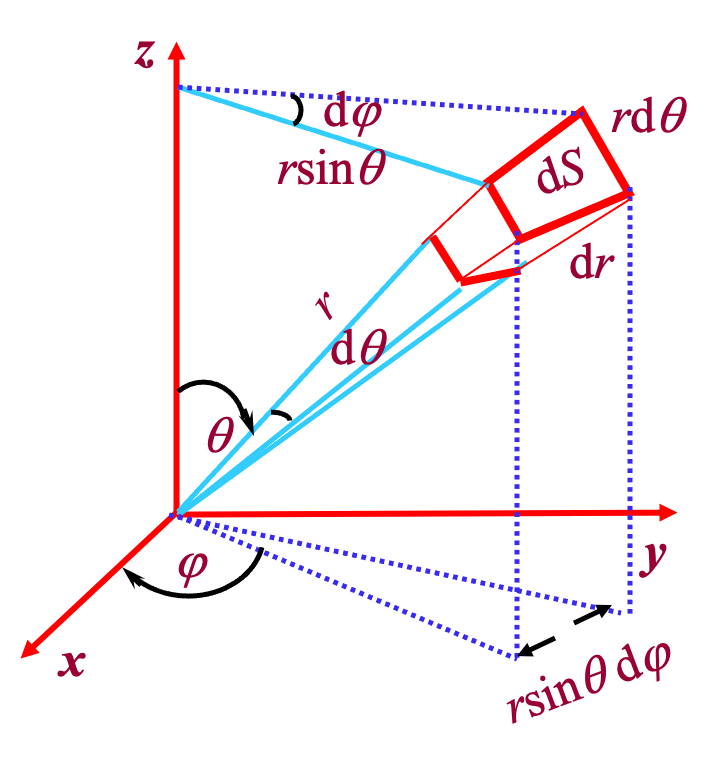
\includegraphics[width=0.4\textwidth]{figs/dt.png}
  \end{center}
$$ \begin{aligned}
  dS&=(rd\theta)\cdot (r\sin \theta d \varphi ) =r^2 \sin \theta d\theta d \varphi \\
  d \tau &=dS \cdot dr = r^2 \sin \theta dr d\theta d \varphi	  
\end{aligned}$$
\end{frame}

\begin{frame}
	* 求 $N_{nl}$ 
	\begin{equation*}
	\begin{split}
		\iiint  &\Psi(r,\theta,\varphi) d \tau =1  \\
		\iiint  &|N_{nl} R (r) Y_{lm} (\theta,\varphi)| ^2 r^2 \sin \theta dr d\theta d\varphi =1  \\
		\int_{0}^{\infty}  & N^2_{nl} R^2  (r)  r^2 dr =1   \\
		\frac{1}{\alpha ^3}	&\int_{0}^{\infty}  N^2_{nl}  R^2 (\xi)  \xi^2 d\xi =1   \\
		\frac{1}{\alpha ^3} &	\int_{0}^{\infty}  N^2_{nl}  \xi ^{2l+2}  [L_{n-l-1} ^{2l+1} (\xi)]^2 e^{-\xi}  d\xi =1   \\
		\frac{1}{\alpha ^3} &	\int_{0}^{\infty}  N^2_{nl}  \xi ^{M+1}  [L_N ^M (\xi)]^2 e^{-\xi}  d\xi =1   \\
	\end{split}		
	\end{equation*}	
\end{frame}		

\begin{frame}
	\begin{equation*}
		\frac{1}{\alpha ^3} 	  N^2_{nl}  \frac{(N+M)!}{N!} (2N+M+1) =1  	
	\end{equation*}	
	$\to$ \\
	\begin{equation*}
		N^2 _{nl}  \frac{2n [(n+1)!]^3} {\alpha^3 (n-l-1)!} =1
	\end{equation*}	
	\begin{equation*}
		N_{nl}  =\sqrt{\alpha^3 \frac{ (n-l-1)!}{2n [(n+1)!]^3}} 
	\end{equation*}	
\end{frame}		

\section{5.氢原子量子描述}

\begin{frame}
	\frametitle{小结:解氢原子}
	\tcbset{enhanced jigsaw,fonttitle=\bfseries,opacityback=0.35,colback=blue!5!white,
		frame style={left color=red!75!black,right color=red!10!yellow}}
	
\begin{tikzpicture}% draw two balls
	  \path[use as bounding box] (0,0.8) rectangle +(0.1,0.1);
	  \shadedraw [shading=ball] (0,0.3) circle (1cm);
	  %\shadedraw [ball color=yellow!20] (3,-2.2) circle (1cm);
	\end{tikzpicture}
	\begin{tcolorbox}[title=\faEnvira\hspace{1em} 第一次分离变量,
	  overlay=
	  {\begin{tcbinvclipframe}
	  \draw[red,line width=1cm] ([xshift=-2mm,yshift=2mm]frame.north west)
	  --([xshift=2mm,yshift=-2mm]frame.south east);
	  \draw[red,line width=1cm] ([xshift=-2mm,yshift=-2mm]frame.south west)
	  --([xshift=2mm,yshift=2mm]frame.north east);
	  \end{tcbinvclipframe}}]
	  {\Bullet}氢原子定态薛定谔方程:
		\begin{equation*}
			\left[-\frac{\hbar^2}{2 m_1} \nabla_1 ^2  -\frac{\hbar^2}{2 m_2} \nabla_2 ^2 +U(| \vec{r_1}-\vec{r_2} | ) \right] \Psi (\vec{r_1},\vec{r_2}) =E \Psi (\vec{r_1},\vec{r_2}) 
		\end{equation*}
	{\Bullet} 质心运动方程
	  \begin{equation*}
		-\frac{\hbar^2}{2 M} \nabla_R ^2  \psi (\vec{R}) =E_c \psi (\vec{R}) 
	\end{equation*}	
	{\Bullet} 相对运动方程
	\begin{equation*}
		\left[-\frac{\hbar^2}{2 m} \nabla ^2 +U(\vec{r}) \right] \Psi (\vec{r}) =E \Psi (\vec{r})   
	\end{equation*}
	  \end{tcolorbox}
\end{frame}

\begin{frame}
	\frametitle{}
	\tcbset{enhanced jigsaw,fonttitle=\bfseries,opacityback=0.35,colback=blue!5!white,
		frame style={left color=red!75!black,right color=red!10!yellow}}
	
\begin{tikzpicture}% draw two balls
	  \path[use as bounding box] (0,0.8) rectangle +(0.1,0.1);
	  \shadedraw [shading=ball] (0,0.3) circle (1cm);
	  %\shadedraw [ball color=yellow!20] (3,-2.2) circle (1cm);
	\end{tikzpicture}
	\begin{tcolorbox}[title=\faEnvira\hspace{1em} 第二次分离变量,
	  overlay=
	  {\begin{tcbinvclipframe}
	  \draw[red,line width=1cm] ([xshift=-2mm,yshift=2mm]frame.north west)
	  --([xshift=2mm,yshift=-2mm]frame.south east);
	  \draw[red,line width=1cm] ([xshift=-2mm,yshift=-2mm]frame.south west)
	  --([xshift=2mm,yshift=2mm]frame.north east);
	  \end{tcbinvclipframe}}]
	{\Bullet}角向方程:
	\begin{equation*}
		\left[ \frac{1}{ \sin \theta  } \frac{\partial }{\partial \theta } (\sin \theta \frac{\partial }{\partial \theta } )
		+\frac{1}{ \sin^2 \theta  } \frac{\partial^2}{\partial\varphi ^2}  +l(l+1) \right] Y=0 
	\end{equation*}
	{\Bullet}径向方程:
	\begin{equation*}
		\frac{d^2 R}{d r^2} + \frac{2}{r^2}\frac{d R }{d r}  + \frac{2 \mu} {\hbar^2}(E+ \frac{e_s ^2}{r} ) R- \frac{l(l+1)}{r^2} R=0
	\end{equation*}	
	  \end{tcolorbox}
\end{frame}

\begin{frame}
	\frametitle{}
	\tcbset{enhanced jigsaw,fonttitle=\bfseries,opacityback=0.35,colback=blue!5!white,
		frame style={left color=red!75!black,right color=red!10!yellow}}
	
\begin{tikzpicture}% draw two balls
	  \path[use as bounding box] (0,0.8) rectangle +(0.1,0.1);
	  \shadedraw [shading=ball] (0,0.3) circle (1cm);
	  %\shadedraw [ball color=yellow!20] (3,-2.2) circle (1cm);
	\end{tikzpicture}
	\begin{tcolorbox}[title=\faEnvira\hspace{1em} 第三次分离变量,
	  overlay=
	  {\begin{tcbinvclipframe}
	  \draw[red,line width=1cm] ([xshift=-2mm,yshift=2mm]frame.north west)
	  --([xshift=2mm,yshift=-2mm]frame.south east);
	  \draw[red,line width=1cm] ([xshift=-2mm,yshift=-2mm]frame.south west)
	  --([xshift=2mm,yshift=2mm]frame.north east);
	  \end{tcbinvclipframe}}]
	{\Bullet}经度方程:
	\begin{equation*}
		\frac{d^{2} \Phi}{d \varphi^{2}}+\lambda \Phi=0,(0<\varphi\le2 \pi)
	\end{equation*}	
	{\Bullet}纬度方程:
	\begin{equation*}
		\frac{1}{\sin \theta} \frac{d}{d \theta}\left(\sin \theta \frac{d \Theta}{d \theta}\right)+\left[l(l+1)-\frac{\lambda}{\sin ^{2} \theta}\right] \Theta=0,(0<\theta \le \pi)
	\end{equation*}	
	{\Bullet}径向方程:
	\begin{equation*}
		\frac{d^2 R}{d r^2} + \frac{2}{r^2}\frac{d R }{d r}  + \frac{2 \mu} {\hbar^2}(E+ \frac{e_s ^2}{r} ) R- \frac{l(l+1)}{r^2} R=0
	\end{equation*}	
	  \end{tcolorbox}
\end{frame}

\begin{frame}
	\frametitle{}
	\tcbset{enhanced jigsaw,fonttitle=\bfseries,opacityback=0.35,colback=blue!5!white,
		frame style={left color=red!75!black,right color=red!10!yellow}}
	
\begin{tikzpicture}% draw two balls
	  \path[use as bounding box] (0,0.8) rectangle +(0.1,0.1);
	  \shadedraw [shading=ball] (0,0.3) circle (1cm);
	  %\shadedraw [ball color=yellow!20] (3,-2.2) circle (1cm);
	\end{tikzpicture}
	\begin{tcolorbox}[title=\faEnvira\hspace{1em} 经度方程的解,
	  overlay=
	  {\begin{tcbinvclipframe}
	  \draw[red,line width=1cm] ([xshift=-2mm,yshift=2mm]frame.north west)
	  --([xshift=2mm,yshift=-2mm]frame.south east);
	  \draw[red,line width=1cm] ([xshift=-2mm,yshift=-2mm]frame.south west)
	  --([xshift=2mm,yshift=2mm]frame.north east);
	  \end{tcbinvclipframe}}]
	{\Bullet}经度方程:
	\begin{equation*}
		\frac{d^{2} \Phi}{d \varphi^{2}}+\lambda \Phi=0,(0<\varphi\le2 \pi)
	\end{equation*}	
	固有值和固有函数:
	\[\begin{cases}
		\lambda=m^2, ~~~ (m=0,\pm 1,\pm 2,\cdots,\pm l) \\ 
		\Phi_m (\varphi)=\frac{1}{\sqrt{2\pi}} e^{im\varphi}
	\end{cases}\]
	物理上对应角动量Z方向投影:
	\[L_z =m\hbar \]
	\end{tcolorbox}
\end{frame}

\begin{frame}
	\frametitle{}
	\tcbset{enhanced jigsaw,fonttitle=\bfseries,opacityback=0.35,colback=blue!5!white,
		frame style={left color=red!75!black,right color=red!10!yellow}}
	
\begin{tikzpicture}% draw two balls
	  \path[use as bounding box] (0,0.8) rectangle +(0.1,0.1);
	  \shadedraw [shading=ball] (0,0.3) circle (1cm);
	  %\shadedraw [ball color=yellow!20] (3,-2.2) circle (1cm);
	\end{tikzpicture}
	\begin{tcolorbox}[title=\faEnvira\hspace{1em} 纬度方程的解,
	  overlay=
	  {\begin{tcbinvclipframe}
	  \draw[red,line width=1cm] ([xshift=-2mm,yshift=2mm]frame.north west)
	  --([xshift=2mm,yshift=-2mm]frame.south east);
	  \draw[red,line width=1cm] ([xshift=-2mm,yshift=-2mm]frame.south west)
	  --([xshift=2mm,yshift=2mm]frame.north east);
	  \end{tcbinvclipframe}}]
	  {\Bullet}纬度方程:
	  \begin{equation*}
		  \frac{1}{\sin \theta} \frac{d}{d \theta}\left(\sin \theta \frac{d \Theta}{d \theta}\right)+\left[l(l+1)-\frac{m^2}{\sin ^{2} \theta}\right] \Theta=0,(0<\theta \le \pi)
	  \end{equation*}	
	固有值
	\[\begin{cases}
		 m^2, ~~~ (m=0,\pm 1,\pm 2,\cdots,\pm l) \\
		l(l+1), ~~~ (l=1, 2,\cdots, n-1) \\ 
	\end{cases}\]
	固有函数:
	\[
		\Theta_{lm}(\theta)= P^m  _{l}(\cos \theta) \]
\end{tcolorbox}
\end{frame}

\begin{frame}
	\frametitle{}
	\tcbset{enhanced jigsaw,fonttitle=\bfseries,opacityback=0.35,colback=blue!5!white,
		frame style={left color=red!75!black,right color=red!10!yellow}}
	
\begin{tikzpicture}% draw two balls
	  \path[use as bounding box] (0,0.8) rectangle +(0.1,0.1);
	  \shadedraw [shading=ball] (0,0.3) circle (1cm);
	  %\shadedraw [ball color=yellow!20] (3,-2.2) circle (1cm);
	\end{tikzpicture}
	\begin{tcolorbox}[title=\faEnvira\hspace{1em} 角向方程的解,
	  overlay=
	  {\begin{tcbinvclipframe}
	  \draw[red,line width=1cm] ([xshift=-2mm,yshift=2mm]frame.north west)
	  --([xshift=2mm,yshift=-2mm]frame.south east);
	  \draw[red,line width=1cm] ([xshift=-2mm,yshift=-2mm]frame.south west)
	  --([xshift=2mm,yshift=2mm]frame.north east);
	  \end{tcbinvclipframe}}]
	{\Bullet}角向方程:
	\begin{equation*}
		\left[ \frac{1}{ \sin \theta  } \frac{\partial }{\partial \theta } (\sin \theta \frac{\partial }{\partial \theta } )
		+\frac{1}{ \sin^2 \theta  } \frac{\partial^2}{\partial\varphi ^2}  +l(l+1) \right] Y=0 
	\end{equation*}
	角动量固有值
	\[\begin{cases}
		m\hbar, ~~~ (m=0,\pm 1,\pm 2,\cdots,\pm l) \\
		l(l+1)\hbar^2, ~~~ (l=1, 2,\cdots, n-1) \\ 
	\end{cases}\]
	固有函数:
	\[
		Y_{lm} (\theta,\varphi)= \sqrt{\frac{(2l+1)(l-m)!}{4\pi (l+m)!}}  P_l ^m (cos \theta)  e^{im\varphi}  \]
\end{tcolorbox}
\end{frame}

\begin{frame}
	\frametitle{}
	\tcbset{enhanced jigsaw,fonttitle=\bfseries,opacityback=0.35,colback=blue!5!white,
		frame style={left color=red!75!black,right color=red!10!yellow}}
	
\begin{tikzpicture}% draw two balls
	  \path[use as bounding box] (0,0.8) rectangle +(0.1,0.1);
	  \shadedraw [shading=ball] (0,0.3) circle (1cm);
	  %\shadedraw [ball color=yellow!20] (3,-2.2) circle (1cm);
	\end{tikzpicture}
	\begin{tcolorbox}[title=\faEnvira\hspace{1em} 径向方程的解,
	  overlay=
	  {\begin{tcbinvclipframe}
	  \draw[red,line width=1cm] ([xshift=-2mm,yshift=2mm]frame.north west)
	  --([xshift=2mm,yshift=-2mm]frame.south east);
	  \draw[red,line width=1cm] ([xshift=-2mm,yshift=-2mm]frame.south west)
	  --([xshift=2mm,yshift=2mm]frame.north east);
	  \end{tcbinvclipframe}}]
	  {\Bullet}径向方程:
	  \begin{equation*}
		\frac{d^2 R}{d r^2} + \frac{2}{r^2}\frac{d R }{d r}  + \frac{2 \mu} {\hbar^2}(E+ \frac{e_s ^2}{r} ) R- \frac{l(l+1)}{r^2} R=0
	  \end{equation*}	
	能量固有值
	\[ E_n =- \frac{1}{n^2} \frac{\mu e^4 _s }{2 \hbar ^2} =\frac{E_1}{n^2}, \qquad (n=1,2,3,\cdots) \]
	固有函数:
	\[
		R_{nl} (r) =\sqrt{(\frac{2}{n a_0})^3 \frac{ (n-l-1)!}{2n [(n+1)!]^3}}  (\frac{2}{n a_0}r) ^l  L_{n-l-1} ^{2l+1} (\frac{2}{n a_0}r) e^{-\frac{r}{n a_0}}\]
\end{tcolorbox}
\end{frame}


\begin{frame}
	\frametitle{}
	\tcbset{enhanced jigsaw,fonttitle=\bfseries,opacityback=0.35,colback=blue!5!white,
		frame style={left color=red!75!black,right color=red!10!yellow}}
	
\begin{tikzpicture}% draw two balls
	  \path[use as bounding box] (0,0.8) rectangle +(0.1,0.1);
	  \shadedraw [shading=ball] (0,0.3) circle (1cm);
	  %\shadedraw [ball color=yellow!20] (3,-2.2) circle (1cm);
	\end{tikzpicture}
	\begin{tcolorbox}[title=\faEnvira\hspace{1em} 氢原子的解,
	  overlay=
	  {\begin{tcbinvclipframe}
	  \draw[red,line width=1cm] ([xshift=-2mm,yshift=2mm]frame.north west)
	  --([xshift=2mm,yshift=-2mm]frame.south east);
	  \draw[red,line width=1cm] ([xshift=-2mm,yshift=-2mm]frame.south west)
	  --([xshift=2mm,yshift=2mm]frame.north east);
	  \end{tcbinvclipframe}}]
	  {\Bullet}	氢原子波函数:
	\begin{equation*}	
		 \Psi_{nlmm_s}(r, \theta, \varphi, s)= R_{nl} (r) Y_{lm} (\theta,\varphi)S_{m_s}(s)
	\end{equation*} 
	\begin{itemize}
		  \item 主量子数: $n=1,2,3,\cdots$, 能级,轨道能量 (主 K,L,M, N, O, P, Q)
		  \item 角量子数: $l=0,1,2,\cdots, n-1$, 角动量大小, 轨道形状 (次 s, p, d, f) 
		  \item 磁量子数: $m=0,\pm 1,\pm 2,\cdots, \pm l$, 角动量方向, 轨道空间取向 
		  \item 自旋量子数: $m_s=\pm 1/2$
	\end{itemize}
\end{tcolorbox}
\end{frame}


\begin{frame}
	  \frametitle{轨道波函数}
	  \begin{center}
		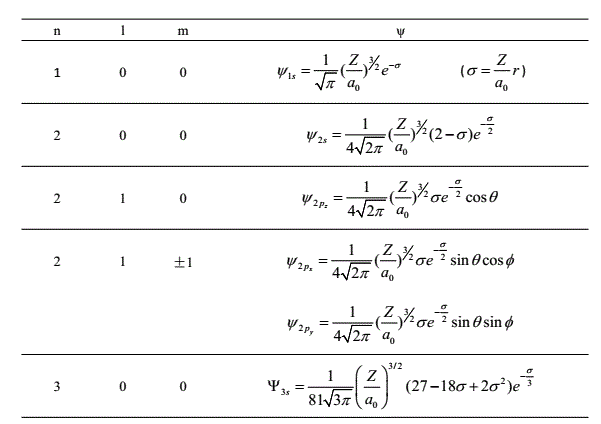
\includegraphics[width=0.95\textwidth]{figs/orbitals.png}
   \end{center}
\end{frame}

\begin{frame}
	  \frametitle{能级与光谱}
	  \[ E_n = - \frac{1}{n^2} \frac{\mu e^4 _s }{2 \hbar ^2} =\frac{E_1}{n^2}, \quad (n=1,2,3,\cdots) , \qquad \nu=\frac{E_n -E_m}{h} = R_H c [\frac{1}{m^2} -\frac{1}{n^2}]
	  \]
	  \begin{center}
		   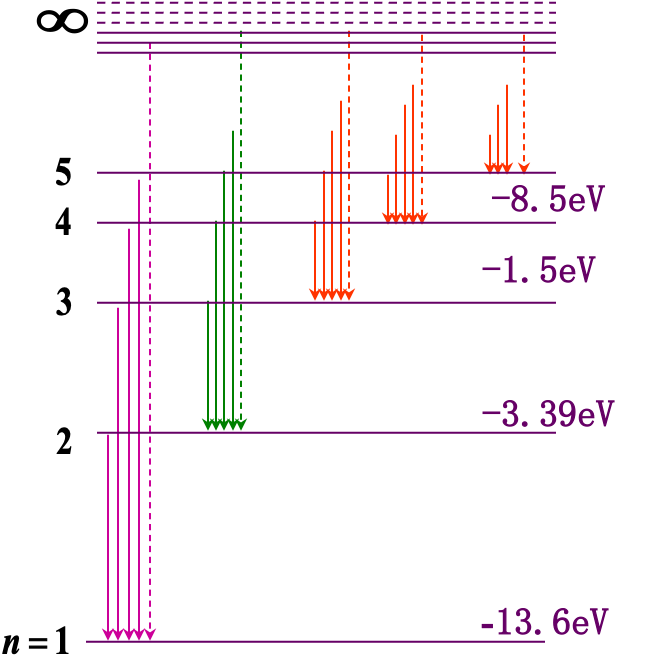
\includegraphics[width=0.40\textwidth]{figs/spectra.png}
	  \end{center}
\end{frame}

\begin{frame} 
    \frametitle{角动量量子化}
    \begin{wrapfigure} {b} {0.4\textwidth} %;图在右
        \includegraphics[width=0.35\textwidth]{figs/LandL2.png}   
    \end{wrapfigure}
    {\Bullet} 角动量大小  $L^2=l(l+1) \hbar^2$\\
	$L=\sqrt{l(l+1)}\hbar, \quad (l=1,2,\cdots, n-1)$\\
    ~~\\ \vspace{0.3em}
    {\Bullet} 角动量Z投影 $L^2_z=m^2\hbar^2$\\
    $L_z=m\hbar, \quad (m=0,\pm 1,\pm 2, \cdots, \pm l)$\\
	~~\\
    {\Bullet} 大小和方向皆量子化
\end{frame} 

\begin{frame}
	  \frametitle{轨道的形态}
		\begin{center}
			 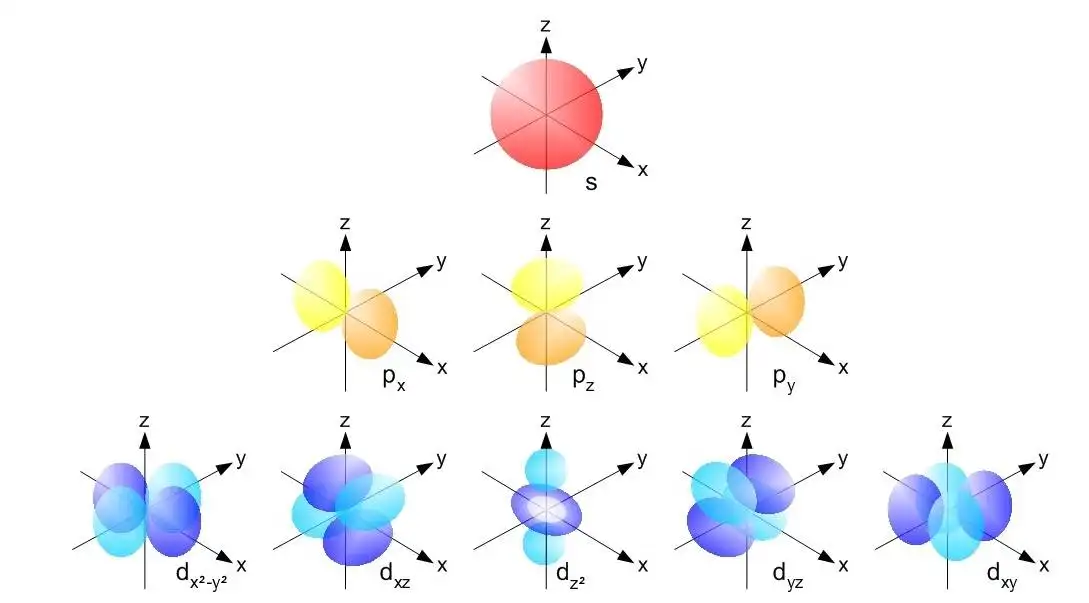
\includegraphics[width=1.0\textwidth,height=2.5in]{figs/2022-03-25-19-35-50.png}
		\end{center}	 
\end{frame}	

\begin{frame}
	  \frametitle{}
	  \例 [求电子云的形态]{}
	  \begin{enumerate}
		  \item 径向分布($r-r+dr$找到粒子的概率)
		   \[ \begin{aligned}
	    \omega_{nl} dr &= \int _{\varphi=0} ^{2\pi} \int _{\theta=0} ^{\pi} |R_{nl}(r)Y_{lm}(\theta,\varphi)|^2 r^2\sin \theta dr d\theta d \varphi \\
		&= R^2_{nl}(r) r^2 dr \\
		\end{aligned}\]
		\item 角向分布($(\theta,\varphi)-(\theta+d\theta,\varphi+d\varphi)$找到粒子的概率)		
		\[ \begin{aligned}
			\omega_{lm} d \Omega &= \int _{r=0} ^{\infty} |R_{nl}(r)Y_{lm}(\theta,\varphi)|^2 r^2dr  d \Omega \\
			&= |Y_{lm}|^2 d \Omega 	
			\end{aligned}\]		
	  \end{enumerate}  
\end{frame}
%%%%%%%%%%%%%%%%%%%%%%%%%%%%%%%%%%%%%%%%%%%%%%
\begin{frame}
	\frametitle{}
  \begin{center}
	   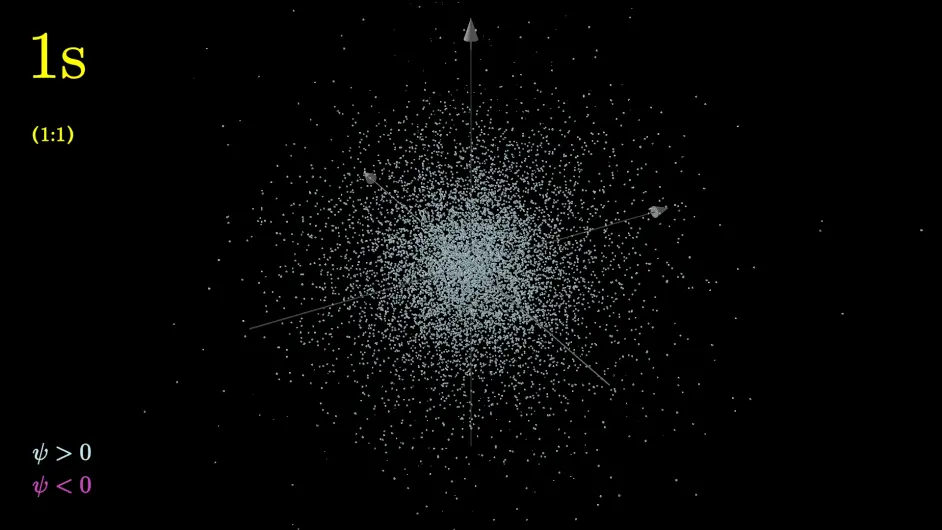
\includegraphics[width=1\textwidth]{figs/2022-03-30-18-45-45.png}
  \end{center}
\end{frame}

\begin{frame}
	\frametitle{}
  \begin{center}
	   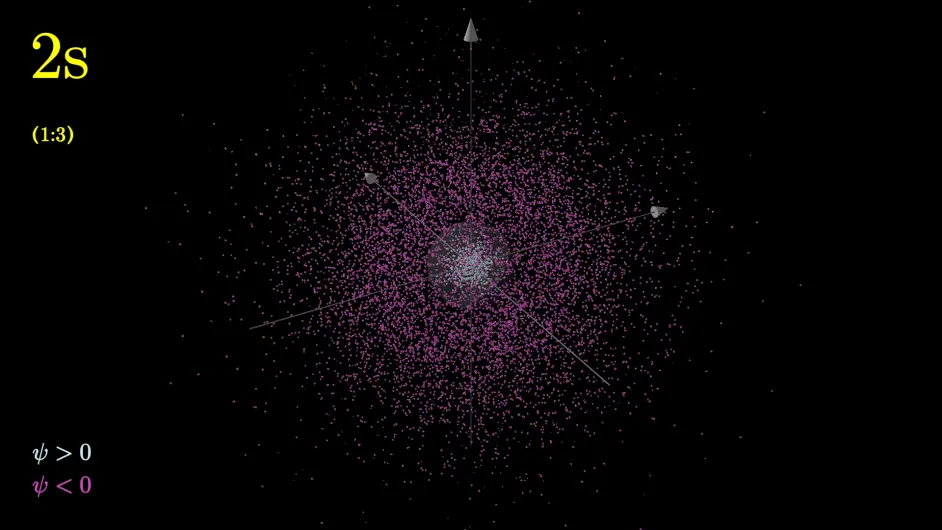
\includegraphics[width=1\textwidth]{figs/2022-03-30-18-46-37.png}
  \end{center}
\end{frame}

\begin{frame}
	\frametitle{}
  \begin{center}
	   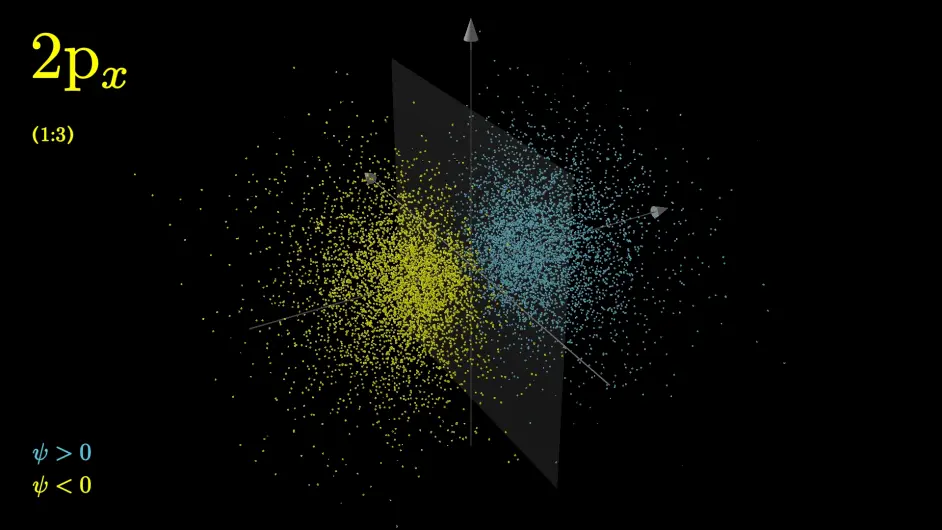
\includegraphics[width=1\textwidth]{figs/2022-03-30-18-48-34.png}
  \end{center}
\end{frame}

\begin{frame}
	\frametitle{}
  \begin{center}
	   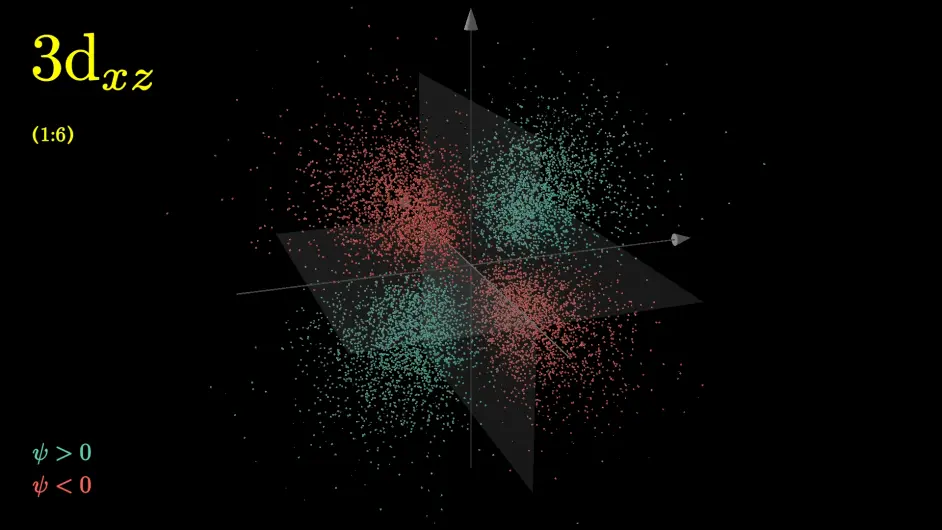
\includegraphics[width=1\textwidth]{figs/2022-03-30-18-49-45.png}
  \end{center}
\end{frame}

\begin{frame}
	\frametitle{}
  \begin{center}
	   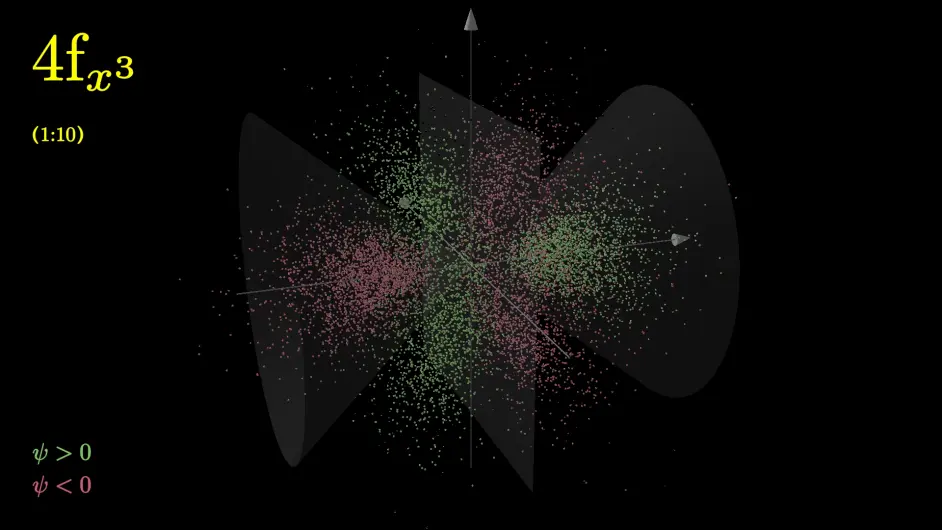
\includegraphics[width=1\textwidth]{figs/2022-03-30-18-55-10.png}
  \end{center}
\end{frame}

\begin{frame}
	\frametitle{作业}
	1、证明拉盖多项式的正交性\\
	2、求方程的解
	\begin{equation*}
		\frac{d^2 U}{d \xi ^2} + \frac{2}{\xi }\frac{d U }{d \xi}  +[\frac{\beta}{\xi} - \frac{l(l+1)}{\xi ^2}] U=0
	\end{equation*}	 
	3、计算积分:
	\begin{equation*}
		\int_{0}^{\infty}   e^{-x} ( L_1 (x) )^2 dx, \qquad  \int_{0}^{\infty}   e^{-x} ( L_2 (x) )^2 dx, 
	\end{equation*}	
	4、写出 $L_1 (x)$ 和 $L_1 ^0 (x)$ 之间的关系式
\end{frame}		

\begin{frame}
	\frametitle{随堂测试}
	\begin{exampleblock} {1.粒子处于如下势场中:}
		\begin{equation*}
			V(x)= \frac{1}{2} \mu \omega ^2 x^2  +1
		\end{equation*}
		\hspace{2em}求能量固有值和定态波函数。
	\end{exampleblock}	
	\begin{exampleblock} {2.基于厄米多项式的正交性求积分:}
		\begin{equation*}
			\int\limits_{-\infty}^{+\infty} (x^3 +1)e^{-x^{2}} H_n(x) d x 
		\end{equation*}
	\end{exampleblock}	
\end{frame}


\begin{frame}
	\frametitle{}
	\begin{exampleblock} {1.粒子处于如下势场中:}
	  \begin{equation*}
		  V(x)= \frac{1}{2} \mu \omega ^2 x^2  +1
	  \end{equation*}
	\end{exampleblock}
	  \hspace{2em}求能量固有值和定态波函数。\\	
	  \解 ~ (1)含时分离变量, 得时间函数: $T(t)  = \exp(-i E t /\hbar) $ \\
	  (2) 定态薛定谔方程:
	  \begin{equation*}
		  \begin{split}
			  \left [ -\frac{\hbar^2}{2\mu} \frac{\mathrm{d} ^2}{\mathrm{d} x^2} +\frac{1}{2}\mu \omega^2 x^2 +1 \right ]\Psi(x)&=E\Psi(x) \\ 
			  \left [ -\frac{\hbar^2}{2\mu} \frac{\mathrm{d} ^2}{\mathrm{d} x^2} +\frac{1}{2}\mu \omega^2 x^2  \right ]\Psi(x)&=(E-1)\Psi(x) 	
		  \end{split}
	  \end{equation*}
	  令 $E'=E-1$, 得:
	  \[\left [ -\frac{\hbar^2}{2\mu} \frac{\mathrm{d} ^2}{\mathrm{d} x^2} +\frac{1}{2}\mu \omega^2 x^2  \right ]\Psi(x)=E'\Psi(x) \]
	  此方程就是谐振子标准方程!
\end{frame}

\begin{frame}
		\frametitle{}	  
	  能量固有值(能级$E_n$)
	  \begin{equation*}
		  E'_n=\left(n+\frac{1}{2}\right) \hbar \omega=E_n-1, ~~~  ( n=0,1,2, ...)  
	  \end{equation*}  
	  定态波函数为
	  \begin{equation*}
		  \Psi_n(x,t) = \left( \frac{\alpha}{\sqrt{\pi} 2^n n!}  \right) ^{1/2}  \exp(-\frac{ \alpha^2 x^2}{2} -\frac{i}{\hbar} E_n t ) H( \alpha x) , \qquad (\alpha ^2= \frac{\mu\omega}{\hbar}) 
	  \end{equation*}  
\end{frame}  
%%%%%%%%%%%%%%%%%%%%%%%%%%%%%%%%%%%%%%%%%%%%%%%%%
\begin{frame}
	\frametitle{}
	\Background[1] 
	\begin{center}
	{ {\Huge 第五章~~贝塞尔函数 (8学时)}}
	\end{center}    
\end{frame}
%%%%%%%%%%%%%%%%%%%%%%%%%%%%%%%%%%%%%%%%%%%%%

\section{1.贝塞尔方程}

\begin{frame}
	\frametitle{方程的建立}
	\begin{exampleblock} {例1、建立贝塞尔方程}
		对于半径为$r_0$的侧面绝缘的薄均匀圆盘,边界温度始终保持为0度,当盘的初始温度已知时 ($\Psi(x,y)$),求体系的温度分布函数。
    \end{exampleblock}
	\begin{center}
		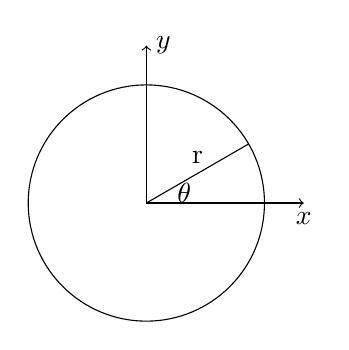
\begin{tikzpicture}
			\def\k{2};
			\node (O) at (0, 0) {};
			\node (A) at (0,1.5) {};
			\node (B) at (30:1.5) {} ;	
			\draw [ ->] (0,0) --  (\k,0)  node[below] {$x$};
			\draw [ ->]  (0,0) -- ( 0,\k)   node[right] {$y$};
			\draw  (0,0) -- (30:1.5) node[midway,above] {r};
			\draw (0,0) circle (1.5cm);
			\path (0,0) ++(15: .5) node{$\theta$};
		\end{tikzpicture}
	\end{center}
\end{frame}	

\begin{frame}
	\alert{ 解:}	这是一个温度场,是非稳恒场,服从热传导方程:\\
	$\begin{cases}
		u_t=a^2 [u_{xx}   +u_{yy}] ~~~~ (0< x^2 +y^2 <r_0 ^2, t>0)\\
		u(x,y,t)|_{x^2+y^2=r_0 ^2}= 0 \\
		u(x,y,t)|_{t=0}= \Psi(x,y)
	\end{cases} $\\	\vspace{0.6em}
	考虑到圆域边界条件,得使用极坐标描述\\
\end{frame}

\begin{frame}
	\frametitle{}
	试证明极坐标拉普拉斯算子为:
	\[[u_{xx}   +u_{yy}]= [ {	\frac{\partial^2 u }{\partial r^2 } +\frac{1}{r } \frac{\partial u }{\partial r } +
	\frac{1}{r^2 } \frac{\partial ^2 u }{\partial \theta ^2
	} }]\]
	\证 ~基本变换关系为 
\[ \begin{cases}
	 x=r\cos \theta\\
	 y=r\sin \theta
	\end{cases}\]
对于函数 $ u(x,y)=u(r\cos \theta,r\sin \theta)$ 计算导数:
\[
\begin{aligned}
	\frac{\partial u}{\partial r}&=\frac{\partial u}{\partial x } \frac{\partial x}{\partial r }+  \frac{\partial u}{\partial y } \frac{\partial y}{\partial r } = \cos \theta \frac{\partial u}{\partial x } +  \sin \theta \frac{\partial u}{\partial y } \\
	\frac{\partial u}{\partial \theta}&=\frac{\partial u}{\partial x } \frac{\partial u}{\partial \theta }+  \frac{\partial u}{\partial y } \frac{\partial y}{\partial \theta } = -r \sin \theta \frac{\partial u}{\partial x } +  r\cos \theta \frac{\partial u}{\partial y } \\
\end{aligned}\]
\end{frame}

\begin{frame}
	改写成矩阵形式:
	\[ 
\begin{aligned}
	&\begin{bmatrix}
	   \frac{\partial u}{\partial r} \\
	   \frac{\partial u}{\partial \theta} 
	\end{bmatrix}
	=
	\begin{bmatrix}
		\cos \theta &  \sin \theta \\
		-r \sin \theta& r\cos \theta \\  
	\end{bmatrix}
	\begin{bmatrix}
		\frac{\partial u}{\partial x} \\
		\frac{\partial u}{\partial y} 
	 \end{bmatrix}\\
	&\begin{bmatrix}
		\frac{\partial u}{\partial r} \\
		\frac{\partial u}{\partial \theta} 
	 \end{bmatrix}
	 =
	 \begin{bmatrix}
		1 &  0 \\
		0 & r \\  
	\end{bmatrix}
	 \begin{bmatrix}
		 \cos \theta &  \sin \theta \\
		 -\sin \theta& \cos \theta \\  
	 \end{bmatrix}
	 \begin{bmatrix}
		 \frac{\partial u}{\partial x} \\
		 \frac{\partial u}{\partial y} 
	  \end{bmatrix}\\
	 &\begin{bmatrix}
		\frac{\partial u}{\partial x} \\
		\frac{\partial u}{\partial y} 
	 \end{bmatrix}
	 =
	 \begin{bmatrix}
		 \cos \theta &  -\sin \theta \\
		 \sin \theta& \cos \theta \\  
	 \end{bmatrix}
	 \begin{bmatrix}
		1 &  0 \\
		0 & 1/r \\  
	\end{bmatrix}
	 \begin{bmatrix}
		 \frac{\partial u}{\partial r} \\
		 \frac{\partial u}{\partial \theta} 
	  \end{bmatrix}\\
\end{aligned}
	  \]
\end{frame}


\begin{frame}
	\frametitle{}
	\[ 
\begin{aligned}
	 &\begin{bmatrix}
		\frac{\partial u}{\partial x} \\
		\frac{\partial u}{\partial y} 
	 \end{bmatrix}
	 =
	 \begin{bmatrix}
		 \cos \theta &  -\sin \theta \\
		 \sin \theta& \cos \theta \\  
	 \end{bmatrix}
	 \begin{bmatrix}
		 \frac{\partial u}{\partial r} \\
		\frac{1}{r} \frac{\partial u}{\partial \theta} 
	  \end{bmatrix}\\
	&\begin{bmatrix}
		\frac{\partial u}{\partial x} \\
		\frac{\partial u}{\partial y} 
	 \end{bmatrix}
	 =
	 \begin{bmatrix}
		 \vec{e}_r & \vec{e}_\theta 
	 \end{bmatrix}
	 \begin{bmatrix}
		 \frac{\partial u}{\partial r} \\
		\frac{1}{r} \frac{\partial u}{\partial \theta} 
	  \end{bmatrix} \\
	&\nabla= \vec{e}_r \frac{\partial }{\partial r} +   \vec{e}_\theta \frac{1}{r} \frac{\partial }{\partial \theta} \\
	&\begin{aligned}
		\nabla ^2 &=\nabla \cdot \nabla \\
		&= (\vec{e}_r \frac{\partial }{\partial r} +   \vec{e}_\theta  \frac{1}{r}\frac{\partial }{\partial \theta})\cdot (\vec{e}_r \frac{\partial }{\partial r} +   \vec{e}_\theta \frac{1}{r} \frac{\partial }{\partial \theta})\\
	\end{aligned}	
\end{aligned}	
	\] 
\end{frame}

\begin{frame}
	\[ \begin{aligned}
	\nabla ^2 &= \vec{e}_r \cdot\frac{\partial }{\partial r}  (\vec{e}_r \frac{\partial }{\partial r} +   \vec{e}_\theta \frac{1}{r} \frac{\partial }{\partial \theta})+  \vec{e}_\theta \cdot \frac{1}{r} \frac{\partial }{\partial \theta} (\vec{e}_r \frac{\partial }{\partial r} +   \vec{e}_\theta \frac{1}{r} \frac{\partial }{\partial \theta})\\
	&=\vec{e}_r \cdot (\frac{\partial \vec{e}_r}{\partial r} \frac{\partial }{\partial r} + \vec{e}_r \frac{\partial ^2 }{\partial r ^2}+  \frac{\partial \vec{e}_\theta}{\partial r} \frac{1}{r}\frac{\partial }{\partial \theta}+  \vec{e}_\theta\frac{\partial }{\partial r} (\frac{1}{r}\frac{\partial }{\partial \theta})) \\
	&\hspace{1em} + \vec{e}_\theta \cdot (\frac{1}{r}\frac{\partial \vec{e}_r}{\partial \theta} \frac{\partial }{\partial r} + \vec{e}_r \frac{1}{r} \frac{\partial }{\partial \theta} \frac{\partial }{\partial r} + \frac{1}{r} \frac{\partial  \vec{e}_\theta}{\partial \theta} \frac{1}{r} \frac{\partial }{\partial \theta} + \vec{e}_\theta \frac{1}{r} \frac{\partial }{\partial \theta} (\frac{1}{r} \frac{\partial }{\partial \theta} )
	) \\
	&=\vec{e}_r \cdot (0 \frac{\partial }{\partial r} + \vec{e}_r \frac{\partial ^2 }{\partial r ^2}+  0\frac{\partial }{\partial \theta}+  \vec{e}_\theta\frac{\partial }{\partial r} (\frac{1}{r}\frac{\partial }{\partial \theta})) \\
	&\hspace{1em} + \vec{e}_\theta \cdot (\vec{e}_\theta \frac{1}{r}\frac{\partial }{\partial r} + \vec{e}_r \frac{1}{r} \frac{\partial }{\partial \theta} \frac{\partial }{\partial r} + \frac{1}{r} (-\vec{e}_r) \frac{1}{r} \frac{\partial }{\partial \theta} + \vec{e}_\theta \frac{1}{r^2} \frac{\partial ^2 }{\partial \theta ^2}
	) \\
	&=  \frac{\partial^2  }{\partial r^2 } +\frac{1}{r } \frac{\partial  }{\partial r } +\frac{1}{r^2 } \frac{\partial ^2  }{\partial \theta ^2} 
	\end{aligned}\] 
~\\ \vspace{1em}
\alert{\textit{Tips:\hspace{1em}}} $\frac{\partial  \vec{e}_\theta}{\partial \theta}=-\vec{e}_r ;\quad \frac{\partial  \vec{e}_\theta}{\partial r}=\vec{e}_\theta ;  \quad \frac{\partial  \vec{e}_r}{\partial r}=0 ; \quad\frac{\partial  \vec{e}_r}{\partial \theta}=0 $ 
\end{frame}

\begin{frame}
	\frametitle{极坐标系下的方程}
	$\begin{cases}
		\displaystyle	u_t=a^2 [ {	\frac{\partial^2 u }{\partial r^2 } +\frac{1}{r } \frac{\partial u }{\partial r } +
		\frac{1}{r^2 } \frac{\partial ^2 u }{\partial \theta ^2
		} }], ~~~~ (0<r<r_0, t>0)\\
		u(r_0,\theta)=0,~~~~~~~~~~~~ 0<\theta <2\pi 	\\
		u(r,\theta,t =0)=\Psi(r,\theta) ,~~~~~~~~~~~~ 0<\theta <2\pi 	
	\end{cases} $\\
	令:$u(r,\theta,t) =R(r)\Theta(\theta)T(t)$,  代回原方程,得:
	\begin{equation*}
		R\Theta T'=a^2 [ R'' \Theta T + \dfrac{1}{r} R' \Theta T  + \dfrac{1}{r^2} R \Theta '' T(t)  ]
	\end{equation*}
	整理:
	\begin{equation*}
		-\frac{T'}{a^2T} =\frac{R''}{R}+\frac{1}{r} \frac{R'}{R} +\frac{1}{r^2} \frac{\Theta ''} {\Theta}  =-\lambda
	\end{equation*}
	转化为两个方程:
	\begin{equation*}
		T'(t)+\lambda a^2T(t)=0  ~~~~~....... ~~~~~~(1)
	\end{equation*}	
	方程1是衰减模型,已求解!\\
\end{frame}	

\begin{frame}
	\begin{equation*}
		r^2 \frac{R'' (r)}{R(r)}+r \frac{R'(r)}{R(r)} + \lambda r^2 +\frac{\Theta ''(\theta)} {\Theta (\theta)} =0  ~~~~~~......~~(2)
	\end{equation*}
	方程2是固有值问题,可继续分离变量:	
	\begin{equation*}
		r^2 \frac{R'' (r)}{R(r)}+r \frac{R'(r)}{R(r)} + \lambda r^2 =-\frac{\Theta ''(\theta)} {\Theta (\theta)} =\mu  
	\end{equation*}
	角向固有值问题:
	$ \begin{cases}
		\Theta ''(\theta)+\mu \Theta (\theta) =0 \\
		\Theta (\theta) =	\Theta (\theta+2\pi)  \\
		\Theta' (\theta) =	\Theta' (\theta+2\pi)  
	\end{cases} $\\	
	径向固有值问题:
	$ \begin{cases}
		r^2 R'' (r)+r R'(r) +( \lambda r^2 -\mu)R(r)=0  \\
		R(r_0)=0
	\end{cases} $\\	
\end{frame}	

\begin{frame}
	角向固有值问题有解,\\
	固有值:
	\begin{equation*}
		\mu=n^2, ~~~~~(n=0,1,2,3...)
	\end{equation*}
	固有函数:
	\begin{equation*}
		\Theta_n(\theta) = a_n \cos(n\theta)+b_n \sin(n\theta), ~~~~~(n=0,1,2,3...)
	\end{equation*}
	\begin{equation*}
		\Theta_n(\theta) = \frac{1}{\sqrt{2\pi}} e^{-i n \theta }, ~~~~~(n=0,1,2,3...)
	\end{equation*}
	~\\
	把$\mu=n^2$,代回径向方程,得径向固有值问题:\vspace{0.6em}
	\[ \boxed{ \begin{cases}
		r^2 R'' (r)+r R'(r) +( \lambda r^2 -n^2)R(r)=0  \\
		R(r_0)=0
	\end{cases} }\]	
	称为贝塞尔方程	
\end{frame}	

\begin{frame}
	\begin{exampleblock} {例2、试证明,圆域波动方程的径向固有值问题也是贝塞尔方程:}~ ~
	\end{exampleblock}
	\证~圆域波动方程如下:\\
	$\begin{cases}
		u_{tt}=a^2 [u_{xx}   +u_{yy}] ~~~~ (0< x^2 +y^2 <r_0 ^2, t>0)\\
		u(x,y,t)|_{x^2+y^2=r_0 ^2}= 0 \\
		u(x,y,t)|_{t=0}= \Psi(x,y) \\
		u_t (x,y,t)|_{t=0}= \varphi  (x,y) 
	\end{cases} $\\	\vspace{0.6em}
	考察方程,发现当使用极坐标拉普拉斯算子后,整个的分离变量过得与热传导方程高度一致,(*P115)\\
	其固有值问题也是贝塞尔方程!\\ \vspace{0.6em}
	$\begin{cases}
		r^2 R'' (r)+r R'(r) +( \lambda r^2 -n^2)R(r)=0  \\
		R(r_0)=0
	\end{cases} $\\		
\end{frame}	

\begin{frame}
	\frametitle{结论: }
	贝塞尔方程是圆域极坐标条件下的一个普适的径向本征方程! \\ \vspace{2em}
	\[\begin{cases}
		r^2 R'' (r)+r R'(r) +( \lambda r^2 -n^2)R(r)=0  \\
		R(r_0)=0
	\end{cases}  \]\\	
\end{frame}	

\begin{frame}	
	在正式求解之前,先预处理一下\\
	令:
	\begin{equation*}
		x=\sqrt{\lambda} r, ~~~~y(x)= R(r) =R(\frac{x}{\sqrt{\lambda}})
	\end{equation*}
	有: 
	\[
	\begin{aligned}
		&\frac{dy}{dx} = \frac{dR}{dr} \frac{dr}{dx} = \frac{1}{ \sqrt{\lambda}} \frac{dR}{dr}\\
		&\frac{d^2y}{dx^2} = \frac{1}{\lambda} \frac{dR^2}{dr^2}\\
	\end{aligned}	
	\]
	代回原方程,
\end{frame}	

\begin{frame}
	得:
	\begin{equation*}
		\boxed{x^2\frac{d^2y}{dx^2} + x\frac{dy}{dx} +(x^2 -n^2)y=0}
	\end{equation*}
	称为n整数阶贝塞尔方程.\\ \vspace{1em}
	{\Bullet}与欧拉方程比较:
	\begin{equation*}
		x^2\frac{d^2y}{dx^2} + x\frac{dy}{dx} +n^2y=0
	\end{equation*}
	欧拉方程是一个变系数微分方程,可通过变量代换(令$t=\ln x $) 转化为常系数微分方程
	\[ \frac{d^2y}{dt^2} - n^2y=0 \]
\end{frame}	

\begin{frame}
	若同样令$t=\ln x $, 贝塞尔方程转化为 
	\[ \frac{d^2y}{dt^2} +(x^2-n^2)y=0 \]
	依然是变系数微分方程,无法进一步进行求解.\\
	因此,贝塞尔方程没有通常意义的初等函数表达式解!
\end{frame}	

\begin{frame}
	\frametitle{方程的求解}
	\begin{exampleblock} {例2、求解贝塞尔方程}
		\begin{equation*}
			x^2\frac{d^2y}{dx^2} + x\frac{dy}{dx} +( x^2 -n^2)y=0
		\end{equation*}	
	\end{exampleblock}
	\alert{ 解:}~没有通常意义的初等函数表达式解,即没有通常意义的级数解,\\
	尝试,设方程有如下非一般意义的级数解:
	\begin{equation*}
		y=\sum\limits_{k=0}^{\infty} a_k x^{s+k},  \qquad (a_0 \not =0)
	\end{equation*}	
\end{frame}	

\begin{frame}
	求导:
	\begin{equation*}
		y'=\sum\limits_{k=0}^{\infty} (s+k) a_k x^{s+k-1}
	\end{equation*}	
	\begin{equation*}
		y''=\sum\limits_{k=0}^{\infty} (s+k) (s+k-1) a_k x^{s+k-2}
	\end{equation*}	
	代回原方程(注意脚标的变化),得:
	\begin{equation*}
		\sum\limits_{k=0}^{\infty} [(s+k) ^2 -n^2]  a_k x^{s+k} + \sum\limits_{k=2}^{\infty}  a_{k-2} x^{s+k} =0
	\end{equation*}	
	第一项(k=0)系数应为零:
	\begin{equation*}
		(s+k) ^2 -n^2=0,~~ \to s_1=-n, \qquad s_2=n. 
	\end{equation*}	
\end{frame}	

\begin{frame}
	第二项(k=1)系数应为零:
	\begin{equation*}
		[(s+k) ^2 -n^2] a_1=0,\qquad \to a_1=0. 
	\end{equation*}	
	后面各项系数都为零:
	\begin{equation*}
		[(s+k) ^2 -n^2] a_k+ a_{k-2}=0, ~~~ (k=2,3,4,...)
	\end{equation*}	
	存在递推关系:
	\begin{equation*}
		a_k=-\frac{1}{(s+k) ^2 -n^2 } a_{k-2}
	\end{equation*}	
	由$a_1=0$,可推出奇数项为零 \[a_{2m+1}=0\]
	现取$s=n$, (-n 不影响解题过程),得:
	\begin{equation*}
		a_{2m}=\frac{-1}{(n+2m) ^2 -n^2 } a_{2m-2} =\frac{-1}{2m (2n+2m) } a_{2m-2}, \qquad (m=1,2,3,...)
	\end{equation*}	
\end{frame}	

\begin{frame}
	归纳,得:
	\begin{equation*}
		a_{2m}=(-1)^m  \frac{1}{2^{2m} m! (n+m) (n+m-1)... (n+1) } a_0 
	\end{equation*}	
	取:$a_0=1/2^n n!$, 得:
	\begin{equation*}
		a_{2m}=(-1)^m  \frac{1}{2^{2m+n} m! (n+m) ! }
	\end{equation*}	
	贝塞尔方程有级数特解:
	\begin{equation*}
		y(x) = \sum\limits_{m=0}^{\infty} a_{2m} x^{n+2m} 
	\end{equation*}	
	分析收敛性,发现:
	\begin{equation*}
		\lim\limits_{m\to \infty}|\frac{ a_{2m+2}} {a_{2m}}|= \lim\limits_{m\to \infty}\frac{ 1}{4(m+1)(n+m+1)} =0
	\end{equation*}	
	说明此级数必为某函数的展开式,称之为贝塞尔函数。
\end{frame}	

\begin{frame}
	记为: \[\boxed{J_n(x) = \sum\limits_{m=0}^{\infty} a_{2m} x^{n+2m}} 
		 \]
	称为n整数阶贝塞尔函数! 
\end{frame}	

\begin{frame}
	\centering
	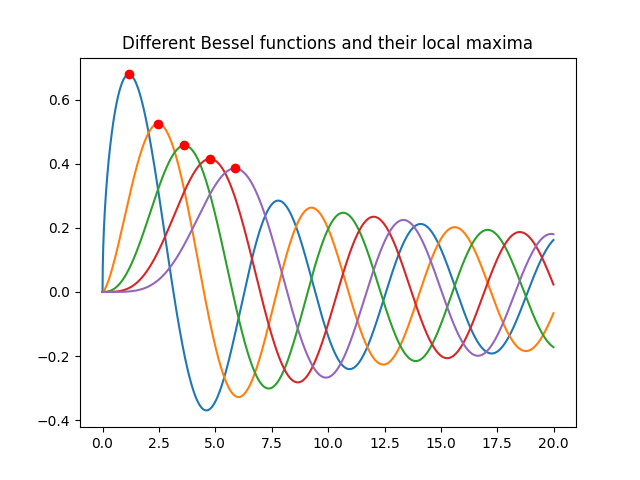
\includegraphics[width=0.8\textwidth]{bessel.png}
\end{frame}	

\begin{frame}
	\begin{center}
		\begin{figure}
			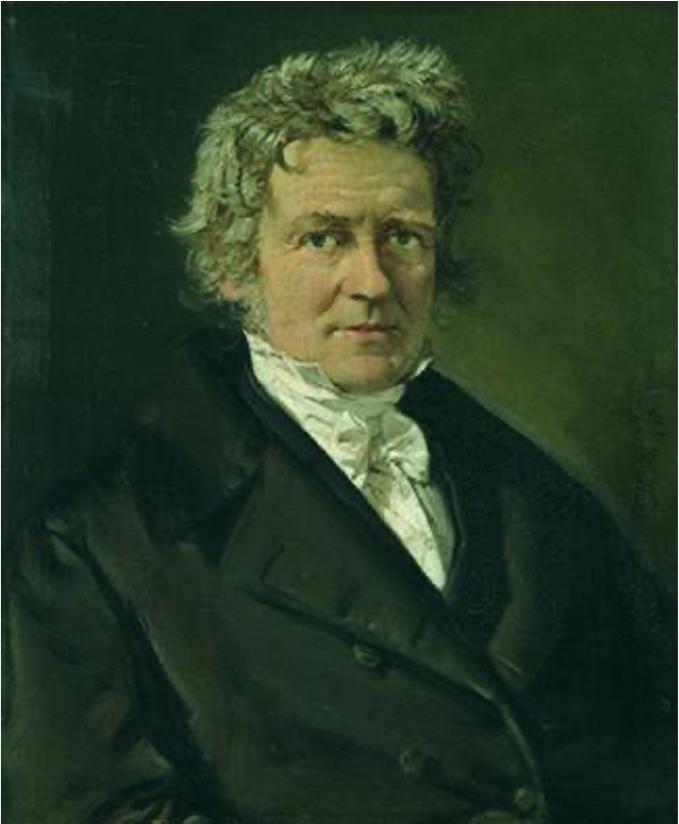
\includegraphics[width=4.2cm]{figs/fig1-3-6.png}	
		\end{figure}
	\end{center}
	贝塞尔(Bessel,Friedrich Wilhelm,1784~1846)德国天文学家,数学家,天体测量学的奠基人.
	提出贝塞尔函数,讨论该函数的一系列性质及其求值方法,为解决物理学、天文学和信息学有关问题提供了重要工具。
\end{frame}

\begin{frame}
	\frametitle{作业}
	1、由圆域波动方程导出贝塞尔方程\\
	2、求衰减模型
	\begin{equation*}
		T'(t)+\lambda a^2T(t)=0  
	\end{equation*}
	3、求角向固有值及归一化的固有函数:\\
	\[ \begin{cases}
		\Theta ''(\theta)+\mu \Theta (\theta) =0 \\
		\Theta (\theta) =	\Theta (\theta+2\pi)  \\
		\Theta' (\theta) =	\Theta' (\theta+2\pi)  
	\end{cases}  \]	
	4、求欧拉方程
\end{frame}	

\section{2.贝塞尔函数与Gamma函数}

\begin{frame}
	\frametitle{贝塞尔函数}
	零阶贝塞尔函数:
	\begin{equation*}
		J_0(x) = \sum\limits_{m=0}^{\infty} (-1)^m  \frac{1}{m! m! } (\frac{x}{2})^{2m} 
	\end{equation*}	
	n阶贝塞尔函数:
	\begin{equation*}
		J_n(x) = \sum\limits_{m=0}^{\infty} (-1)^m  \frac{1}{m! (n+m) ! } (\frac{x}{2})^{n+2m} 
	\end{equation*}	
	第二类塞尔函数:
	\begin{equation*}
		Y_{\alpha}(x)=\frac{J_{\alpha}(x) \cos (\alpha \pi)-J_{-\alpha}(x)}{\sin (\alpha \pi)}
	\end{equation*}	
	贝塞尔函数在除$x=0$点外的整个实数轴上收敛。
\end{frame}	

\begin{frame}
	\frametitle{$\Gamma$函数定义}
	为进一步讨论贝塞尔函数的性质,先由Euler积分定义Gamma函数
	\begin{equation*}
		\Gamma(x)=\int_{0}^{\infty} t^{x-1} e^{-t} dt, \qquad (x>0)
	\end{equation*}	
	是Euler创造出来将积分和阶乘联系起来的一个函数\\ \vspace{0.6em}
	\例 [1.试证明]
	{ \[
		\Gamma(1)=1
	   \]}
	\证 ~	
\[ \begin{aligned}
	\Gamma(1)&=\int_{0}^{\infty} t^{1-1} e^{-t} dt \\	
			&=\int_{0}^{\infty}  e^{-t} dt =1	
\end{aligned}\]
\end{frame}	

\begin{frame}	
	\frametitle{~$\Gamma$函数的性质}
	\alert{性质1:} ~试证明Gamma函数有如下递推式:\\
		$\Gamma(x+1)=x \Gamma(x),\qquad (x>0)$\\
	\alert{证明:}  
	\begin{equation*}
	\begin{split}
		\Gamma(x+1)&= \int_{0}^{\infty} t^{x} e^{-t} dt \\
		&= -t^x e^{-t} |_0 ^\infty + x \int_{0}^{\infty} t^{x-1} e^{-t} dt \\
		&= x \int_{0}^{\infty} t^{x-1} e^{-t} dt \\
		&=x \Gamma(x)
	\end{split}
	\end{equation*}	
\end{frame}	

\begin{frame}
	 推论: 
	\begin{equation*}
		\Gamma(x+n)=(x+n-1)(x+n-2)\cdots (x+1)x\Gamma(x)
	\end{equation*}	 \vspace{2cm}
\end{frame}	

\begin{frame}
	\alert{性质2:}~试证明自变量为正整数的Gamma函数有如下形式:
	\begin{equation*}
		\Gamma(n+1)=n!
	\end{equation*}	
	\alert{证明:}  由递推公式
	\begin{equation*}
	\begin{split}
		\Gamma(x+1)&=x \Gamma(x) \\
		\Gamma(n+1)&=n \Gamma(n) \\
		&=n(n-1)\cdots 1 \Gamma(1) \\
		&=n! \int_{0}^{\infty}  e^{-t} dt \\
		&=n!
	\end{split}
	\end{equation*}	
\alert{\textit{Tips:\hspace{1em}}} ~ 阶乘只是$\Gamma(x)$函数的特例!$(x=1,2,3,\cdots)$
\end{frame}	

\begin{frame}
	\alert{性质3:} ~Gamma函数在非正整数点的极限为无穷大
	\begin{equation*}
		\lim\limits_{x\to -n }\Gamma(x)=\infty, \qquad (n=0,1,2, \cdots)
	\end{equation*}	
	\alert{证明:}  由递推公式
	\begin{equation*}
	\begin{split}
		\Gamma(x)&=\frac{1}{x} \Gamma(x+1) \\
		\lim\limits_{x\to 0 }	\Gamma(x)&=	\lim\limits_{x\to 0 } \frac{1}{x} \Gamma(x+1) =\infty \\
		\lim\limits_{x\to -1 }	\Gamma(x)&=\lim\limits_{x\to -1 } \frac{1}{x} \Gamma(x+1) =  \lim\limits_{x\to 0 } \frac{1}{x-1} \Gamma(x) =\infty \\
		& \cdots \cdots \\
		\lim\limits_{x\to -n }	\Gamma(x)&=\lim\limits_{x\to -n } \frac{1}{x} \Gamma(x+1) = \lim\limits_{x\to -(n-1) } \frac{1}{x-1} \Gamma(x) =\infty \\
	\end{split}
	\end{equation*}	
\end{frame}	

\begin{frame}
	 推论: 
	\begin{equation*}
		\frac{1}{\Gamma(-n)} =0, \qquad (n=0,1,2, \cdots)
	\end{equation*}	 \vspace{2cm}
\end{frame}	

\begin{frame}
	\alert{性质4:} 试证明半正整数$\Gamma$函数有如下性质 
	\begin{equation*}
		\begin{split}
		\Gamma(\frac{1}{2}) &=\sqrt{\pi} \\ 
		\qquad  \Gamma(n+\frac{1}{2}) &= \frac{(2n-1)!!}{2^n} \sqrt{\pi}
		\end{split}	
	\end{equation*}	
	\alert{证明:}  由Gamma函数定义
	\[
	\begin{aligned}
		 \Gamma(x)&=\int_{0}^{\infty} t^{x-1} e^{-t} dt, \qquad (x>0) \\
		 \Gamma(\frac{1}{2})&=\int_{0}^{\infty} t^{\frac{1}{2}-1} e^{-t} dt\\
		 &=\int_{0}^{\infty} \frac{1}{\sqrt{t}} e^{-t} dt\\
	\end{aligned}	
	\]
\end{frame}

\begin{frame}
	  \frametitle{}
	  令$x=\sqrt{t}$
	  \[
		\begin{aligned}
			 \Gamma(\frac{1}{2})
			 &=2\int_{0}^{\infty} e^{-x^2} dx\\
			 &=2\sqrt{\iint_{0}^{\infty} e^{-x^2} e^{-y^2} dxdy}\\
			 &=2\sqrt{\int_{0}^{\frac{\pi}{2}} d\theta \int_{0}^{\infty}  e^{-r^2} r dr }\\
			 &=2\sqrt{\frac{\pi}{2}\int_{0}^{\frac{\pi}{2}} \int_{0}^{\infty} r e^{-r^2} dr d\theta}\\
			 &=2\sqrt{\frac{\pi}{2}[-\frac{1}{2} e^{-r^2}]_{0}^{\infty} }\\
			 &=\sqrt{\pi}
		\end{aligned}	
		\]  
	* 第一象限!			
\end{frame}	

\begin{frame}
	  \frametitle{}
	  由递推公式 $\Gamma(1+x)=x \Gamma(x) ,\qquad (x>0)$\\
	  \[
	\begin{aligned}
		\Gamma(1+\frac{1}{2})&= \frac{1}{2} \Gamma(\frac{1}{2}) =\frac{1}{2} \sqrt{\pi}\\
		\Gamma(2+\frac{1}{2})&= \Gamma(1+\frac{3}{2})=\frac{3}{2} \Gamma(1+\frac{1}{2}) = \frac{3}{2}\frac{1}{2}\sqrt{\pi}\\
		\Gamma(3+\frac{1}{2})& = \frac{5}{2} \frac{3}{2}\frac{1}{2}\sqrt{\pi}\\
		\Gamma(n+\frac{1}{2})& = \frac{(2n-1)!!}{2^n}\sqrt{\pi}\\
		 & = \frac{(2n)!}{2^{2n} n!}\sqrt{\pi}
	\end{aligned} 
	  \]
	证毕!

\end{frame}


\begin{frame}
	\alert{推论:} 半正整数的阶乘
	\[ \begin{aligned}
		(m-\frac{1}{2})! &= \Gamma (m-\frac{1}{2}+1) \\
						 &= \Gamma (m+\frac{1}{2}) \\
						 & = \frac{(2m)!}{2^{2m} m!}\sqrt{\pi} \\
		(\frac{1}{2})! &=  \frac{\sqrt{\pi}}{2} \\
	\end{aligned} \]
	~\\
* 一般分数的阶乘如何求?(余元公式,自己证明!)
\[ \Gamma(x)  \Gamma(1-x) =\frac{\pi}{\sin x \pi}, \qquad  0<x<1 \]
\[ \Gamma(\frac{1}{2}+x)  \Gamma(\frac{1}{2}-x) =\frac{\pi}{\cos x \pi}, \qquad  0<x<\frac{1}{2} \]
\end{frame}

\begin{frame}
	\alert{性质5:} 试求负半正整数$\Gamma$函数的值
	\begin{equation*}
		\begin{split}
		\Gamma(-\frac{1}{2}) &=-2\sqrt{\pi} \\ 
		\Gamma(-\frac{3}{2}) &=\frac{4}{3}\sqrt{\pi}
		\end{split}	
	\end{equation*}	
	\alert{解:} (1) 在递推公式 $\Gamma(1+x)=x \Gamma(x)$中, 令$x=-\dfrac{1}{2}$\\
	\[
	\begin{aligned}
		 \Gamma(-\frac{1}{2})&= -2 \Gamma(1-\frac{1}{2})\\
		 &=-2 \Gamma(\frac{1}{2})\\
		 &=-2 \sqrt{\pi}
	\end{aligned}	
	\]
\end{frame}

\begin{frame}
	  \frametitle{}
	(2) 在递推公式 $\Gamma(1+x)=x \Gamma(x)$中, 令$x=-\dfrac{3}{2}$\\
	\[
	\begin{aligned}
		 \Gamma(-\frac{3}{2})&= -\frac{2}{3} \Gamma(1-\frac{3}{2})\\
		 &=-\frac{2}{3} \Gamma(-\frac{1}{2})\\
		 &=(-\frac{2}{3})(-2 \sqrt{\pi}) \\
		 &=\frac{4}{3}\sqrt{\pi} \\
	\end{aligned}	
	\] ~\\
\end{frame}

\begin{frame}
	\frametitle{}
  \begin{center}
	   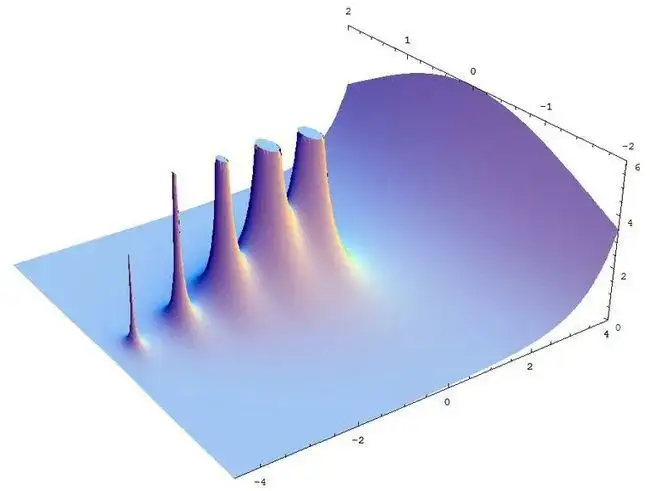
\includegraphics[width=0.85\textwidth,height=2.7in]{figs/2022-03-26-17-20-10.png}
  \end{center}
  \alert{\textit{Tips:\hspace{1em}}} $\Gamma$把阶乘延拓到实数域后, 依然有$x \not = 0,-1,-2,\cdots$, 
进一步延拓到复数域后, 这些奇点依然存在!
\end{frame}

%%%%%%%%%%%%%%%%%%%%%%%%%%%%%%%%%%%%%%%%%%%%%%%%%%%%%%%%%%%%%%%%%%%
\begin{frame}
	\frametitle{课外作业}
	试证明如下量子力学里常用的计算公式
	\begin{enumerate}
		\item $ \int_{-\infty}^{\infty} e^{-\alpha x^{2}} d x=\sqrt{\frac{\pi}{\alpha}}$
		\item $\int_{0}^{\infty} x^{m} e^{-\alpha x} d x=\frac{m !}{\alpha^{m+1}}$ 
		\item $ \int_{-\infty}^{\infty} x^{2 n} e^{-\alpha x^{2}} d x=\frac{1.3 .5 \cdot \cdots(2 n-1)}{(2 \alpha)^{n}} \sqrt{\frac{\pi}{\alpha}}$
		\item $ \int_{-\infty}^{\infty} e^{-a x^{2}+b x} d x=\sqrt{\frac{\pi}{a}} e^{\frac{b^{2}}{4 a}}$
	\end{enumerate}
\end{frame}
%%%%%%%%%%%%%%%%%%%%%%%%%%%%%%%%%%%%%%%%%%%%%%%%%%%%%%%%%%%%%%%%%%%

\section{3.贝塞尔函数的性质}

\begin{frame}
	现在讨论贝塞尔函数的性质:\\
	\alert{性质1:} 负数阶贝塞尔函数与正数阶贝塞尔函数有如下关系
	\begin{equation*}
		J_{-n}(x)=(-1)^n J_n(x)
	\end{equation*}	
	\alert{证明:}  
	用$\Gamma$ 函数重写出贝塞尔函数:
	\begin{equation*}
		J_n(x) = \sum\limits_{m=0}^{\infty} (-1)^m  \frac{1}{m! (n+m) ! } (\frac{x}{2})^{n+2m} 
	\end{equation*}	
	\begin{equation*}
		J_n(x) = \sum\limits_{m=0}^{\infty} (-1)^m  \frac{1}{m! \Gamma(n+m+1) } (\frac{x}{2})^{n+2m} 
	\end{equation*}	
	负数阶塞尔函数可写成
	\begin{equation*}
		J_{(-n)}(x) = \sum\limits_{m=0}^{\infty} (-1)^m  \frac{1}{m! \Gamma(-n+m+1) } (\frac{x}{2})^{-n+2m} 
	\end{equation*}	
\end{frame}	

\begin{frame}
	对于 $m<n$ 的项,由于分母中的Gamma函数为无穷大,所以都为零:
	\begin{equation*}
		J_{(-n)}(x) = \sum\limits_{m=n}^{\infty} (-1)^m  \frac{1}{m! \Gamma(-n+m+1) } (\frac{x}{2})^{-n+2m} 
	\end{equation*}	
	令 $m-n=k$, 有 $m=n+k $, 
	\begin{equation*}
		J_{(-n)}(x) = (-1)^n\sum\limits_{k=0}^{\infty} (-1)^k  \frac{1}{(n+k)! \Gamma(k+1) } (\frac{x}{2})^{n+2k} 
	\end{equation*}	
	\begin{equation*}
		J_{-n} (x) = (-1)^n\sum\limits_{k=0}^{\infty} (-1)^k  \frac{1}{(n+k)! k! } (\frac{x}{2})^{n+2k} =(-1)^n J_{n} (x)
	\end{equation*}	
\end{frame}	

\begin{frame}
	\alert{性质2:} 半整数阶贝塞尔函数与三角函数有如下关系
	\begin{equation*}
		J_{1/2} (x) =\sqrt{\frac{2}{\pi x}} \sin x,  \qquad  J_{-1/2} (x) =\sqrt{\frac{2}{\pi x}} \cos x
	\end{equation*}	
	\alert{证明:}  基于Gamma函数,可以写出半整数阶贝塞尔函数
	\begin{equation*}
		J_n(x) = \sum\limits_{m=0}^{\infty} (-1)^m  \frac{1}{m! \Gamma(n+m+1) } (\frac{x}{2})^{n+2m} 
	\end{equation*}	
	\begin{equation*}
		J_{1/2}(x) = \sum\limits_{m=0}^{\infty} (-1)^m  \frac{1}{m! \Gamma(1/2+m+1) } (\frac{x}{2})^{1/2+2m} 
	\end{equation*}	
\end{frame}	

\begin{frame}
	其中, 
	\begin{equation*}
		\begin{split}
			\Gamma(1/2+m+1) &= (\frac{2m+1}{2}) \Gamma(1/2+m) \\
			& = (\frac{2m+1}{2}\frac{2m-1}{2})  \Gamma(1/2+m-1) \\
			&\cdots \cdots \\
			& = \frac{(2m+1)!!}{2^{m+1}} \Gamma(1/2) \\
			& = \frac{(2m+1)!!}{2^{m+1}} \sqrt{\pi} \\
		\end{split}	
	\end{equation*}	
\end{frame}	

\begin{frame}
	代回,有:
	\begin{equation*}
		J_{1/2}(x) = \sqrt{\frac{2}{\pi x}} \sum\limits_{m=0}^{\infty} (-1)^m  \frac{x^{2m+1}}{(2m+1)!} 
	\end{equation*}	 
	\begin{equation*}
		J_{1/2}(x) = \sqrt{\frac{2}{\pi x}} \sin x  
	\end{equation*}	 
	同理,有  
	\begin{equation*}
		J_{-1/2}(x) = \sqrt{\frac{2}{\pi x}} \cos x  
	\end{equation*}	 
	\alert{证毕!} 
\end{frame}

\begin{frame}
	\frametitle{作业}
	1、证明 \[ \Gamma(1/2)=\sqrt{\pi}\]
	2、证明
	\begin{equation*}
		J_{-1/2}(x) = \sqrt{\frac{2}{\pi x}} \cos x  
	\end{equation*}
\end{frame}

\begin{frame}
	\alert{性质3:} 贝塞尔函数的导数与递推式 \\
	\begin{equation*}
		\begin{split}
			\frac{d}{d x}\left[x^{n} J_{n}(x)\right]= &x^{n} J_{n-1}(x) \\
			\frac{d}{d x}\left[x^{-n} J_{n}(x)\right]=& -x^{-n} J_{n+1}(x) \\
			2 n J_{n}(x)=&xJ_{n-1}(x)+x J_{n+1}(x) \\
			2 J_{n}^{\prime}(x)=&J_{n-1}(x)-J_{n+1}(x)
		\end{split}
	\end{equation*}		
	\alert{证明:}
	\begin{equation*}
		J_n(x) = \sum\limits_{m=0}^{\infty} (-1)^m  \frac{1}{m! \Gamma(n+m+1) } (\frac{x}{2})^{n+2m} 
	\end{equation*}	 
	等于两端乘以$x^n$ 再求导:
	\begin{equation*}
	\begin{split}
		\frac{d}{dx} [x^n J_n(x)]&= \frac{d}{dx}\sum\limits_{m=0}^{\infty} (-1)^m  
		\frac{1}{m! \Gamma(n+m+1) } (\frac{x^{2n+2m}}{2^{n+2m}})\\	
	\end{split}
	\end{equation*}		
\end{frame}	

\begin{frame}
	\begin{equation*}
		\begin{split}
			\frac{d}{dx} [x^n J_n(x)] &=\sum\limits_{m=0}^{\infty} (-1)^m  
			\frac{1}{m! \Gamma(n+m+1) } (\frac{(2n+2m)x^{2n-1+2m}}{2^{n+2m}})\\
			&=x^n\sum\limits_{m=0}^{\infty} (-1)^m  
			\frac{1}{m! \Gamma(n-1+m+1) } (\frac{x^{n-1+2m}}{2^{n-1+2m}})\\ 
			&=x^n J_{n-1}(x)
		\end{split}
	\end{equation*}	
	同理,得:
	\begin{equation*}
		\begin{split}
		\frac{d}{d x}\left[x^{-n} J_{n}(x)\right]&=-x^{-n} J_{n+1}(x) \\
		\end{split}
	\end{equation*}	 
	把上二式左端求导,然后相加相减,得
	\begin{equation*}
		\begin{split}
		2 n J_{n}(x)=&x J_{n-1}(x)+x J_{n+1}(x) \\
		2 J_{n}^{\prime}(x)=&J_{n-1}(x)-J_{n+1}(x)
		\end{split}
	\end{equation*}	 	
\end{frame}

\begin{frame}
	\alert{性质4:} 贝塞尔函数的零点\\
	\alert{解:}对n(整数)阶贝塞尔方程
	\begin{equation*}
		x^2\frac{d^2y}{dx^2} + x\frac{dy}{dx} +(x^2 -n^2)y=0
	\end{equation*}
	做变量代换 \[ y=\frac{u}{\sqrt{x}}\] 
	得到 u(x)的方程:
	\begin{equation*}
		u'' +[1+\frac{\frac{1}{4}-n^2}{x^2}] u=0
	\end{equation*}
	当$x \to \infty $ 有方程:
	\begin{equation*}
		u'' + u=0 
	\end{equation*}	
\end{frame}	

\begin{frame}
	通解为:\[u=A\cos(x+\theta)\]
	确定A和$\theta$,得n阶贝塞尔函数的渐近公式\\
	\begin{equation*}
		J_{n}(x) \approx \sqrt{\frac{2}{\pi x}} \cos \left(x-\frac{n \pi}{2}-\frac{\pi}{4}\right)
	\end{equation*}
	得零点近似公式:
	\begin{equation*}
		\mu_{m}^{n} \approx m \pi+\frac{n \pi}{2}+\frac{3 \pi}{4}
	\end{equation*}
	对于热传导方程和波动方程,其解为n阶贝塞尔函数$J_n(x)$
	\[\begin{cases}
		r^2 R'' (r)+r R'(r) +( \lambda r^2 -n^2)R(r)=0  \\
		R(r_0)=0
	\end{cases}  \]
	对于零边界条件$J_n(\sqrt{\lambda}r_0)=0$, 正是求贝塞尔函数的零点
\end{frame}	

\begin{frame}
	基此可确定:\\	
	(1)固有值:
	\[ \sqrt{\lambda}r_0 = \mu_{m}^{n}  \qquad \to \qquad \lambda_m ^n =(\frac{\mu_{m}^{n}}{r_0})^2 \]
	(2)固有函数:\[R_m ^n(r) = J_n (\frac{\mu_{m}^{n}}{r_0}r) \]
\end{frame}

\begin{frame}
	\alert{性质5:} 贝塞尔函数正交归一性\\
	固有函数体现塞尔函数的正交归一性:
	\begin{equation*}
		\int_0 ^{r_0} r J_n (\frac{\mu_{m} ^{n}}{r_0}r) J_n (\frac{\mu_{k} ^{n}}{r_0}r) dr =?
	\end{equation*}
	\alert{证明:}对径向方程做等价变换
	\begin{equation*}
		r^2 R''+r R' +(\lambda r^2 -n^2)R=0 
	\end{equation*}	
	\begin{equation*}
		r R''+ R' +((\frac{\mu_{m}^{n}}{r_0})^2 r -\frac{n^2}{r})R=0  
	\end{equation*}	
	\begin{equation*}
		(r R')' +((\frac{\mu_{m}^{n}}{r_0})^2 r -\frac{n^2}{r})R=0  
	\end{equation*}	
\end{frame}	

\begin{frame}
	令:\[J_n (\frac{\mu_{m}^{n}}{r_0}r)=R_1, \qquad J_n (\frac{\mu_{k}^{n}}{r_0}r) =R_2\]
	有
	\begin{equation*}
		(r R_1')' +((\frac{\mu_{m}^{n}}{r_0})^2 r -\frac{n^2}{r})R_1=0  \cdots (1)
	\end{equation*}	 
	\begin{equation*}
		(r R_2')' +((\frac{\mu_{m}^{n}}{r_0})^2 r -\frac{n^2}{r})R_2=0  \cdots (2) 
	\end{equation*}	
	$(1)\times R_2,  (2)\times R_1,$所得两次相减,并做积分,有
	\begin{equation*}	
		\int_0 ^{r_0} \left[\left(\frac{\mu_{m}^{(n)}}{r_0}\right)^{2}-\left(\frac{\mu_{k}^{(n)}}{r_0}\right)^{2}\right] r R_{1} R_{2} dr 
		=\int_0 ^{r_0}  [R_{1}\left(r R_{2}^{\prime}\right)^{\prime}-R_{2}\left(r R_{1}^{\prime}\right)^{\prime}] dr
	\end{equation*}
\end{frame}	

\begin{frame}
	\begin{equation*}
		\begin{split}
			=& [r R_1 R_2']|_0 ^{r_0} - [r R_2 R_1']|_0 ^{r_0} + \int_0 ^{r_0} r R_2' R_1 dr - \int_0 ^{r_0} rR_1' R_2 dr\\
			=& \int_0 ^{r_0} rR_2'R_1 dr - \int_0 ^{r_0} rR_1'R_2 dr\\
			=& 0
		\end{split}
	\end{equation*}	
	\begin{equation*}	
		\to \qquad	\int_0 ^{r_0} r R_{1} R_{2} dr = 0
	\end{equation*}
	正交性,\alert{证毕!}
\end{frame}	

\begin{frame}
	下面证明归一性:
	\begin{equation*}
		r^2 R''+r R' +(\lambda r^2 -n^2)R=0 
	\end{equation*}	
	\begin{equation*}
		2r^2 R'R''+2r (R')^2 +(\lambda r^2 -n^2)R'R=0 
	\end{equation*}	
	 整理:
	\begin{equation*}
		[r^2 (R')^2 + (\lambda r^2 -n^2)R^2]'=2 \lambda rR^2
	\end{equation*}	
\end{frame}	

\begin{frame}
	\begin{equation*}
		\begin{split}
			\int_0 ^{r_0} r R^2 dr =& \frac{1}{2\lambda} \int_0 ^{r_0} [r^2 (R')^2 + (\lambda r^2 -n^2)R^2]' dr  \\
			=& \frac{1}{2\lambda} |r^2 (R')^2 + (\lambda r^2 -n^2)R^2 |_0 ^{r_0} \\
			=& \frac{1}{2\lambda} r_0^2 (R'(r_0))^2 \\
			=& \frac{1}{2} r_0^2 [J'_n(\mu_m ^n)]^2 \\
			=& \frac{r_0^2}{2} [J_{n+1}(\mu_m ^n)]^2
		\end{split}
	\end{equation*}	
\end{frame}	

\section{4.贝塞尔函数的应用}
\begin{frame}
	\frametitle{应用实例}
	求解圆域热传导问题 \\
	$\left\{
		\begin{array}{l}
		\dfrac{\partial u}{\partial t}=a^{2}\left(\dfrac{\partial^{2} u}{\partial r^{2}}+\dfrac{1}{r} 
		\dfrac{\partial u}{\partial r}+\dfrac{1}{r^{2}} \dfrac{\partial^{2} u}{\partial \theta^{2}}\right), 0<r<R, 0<\theta<2 \pi \\
		\left. u\right|_{r=R}=0,\left.u\right|_{t=0}=\varphi(r, \theta)
	\end{array}
	\right. $\\
	\alert{解:} 令 
	\begin{equation*}
		u(r,\theta,t)= T(t) V(r, \theta) 
	\end{equation*}	
	代入方程,进行第一次分离变量,得衰减方程:\[T'+\lambda a^2 T=0, \qquad \cdots (1) \]	
\end{frame}

\begin{frame}
	及亥姆霍兹方程:
	$\left\{
	\begin{array}{l}
		\frac{\partial^{2} V}{\partial r^{2}}+\frac{1}{r} \frac{\partial V}{\partial r}+\frac{1}{r^{2}} 
		\frac{\partial^{2} V}{\partial \theta^{2}}+\lambda V=0, 0<r<R, 
		0 \leq \theta \leq 2 \pi \\
		\left.V\right|_{r=R}=0, 0 \leq \theta \leq 2 \pi
		\end{array}
	\right.$\\
	令\[V(r, \theta) =F(r)G(\theta)\], 代入亥姆霍兹方程, 得两个方程\\
	\[G''+\mu G=0, \qquad \cdots (2) \]
	\[r^2 F''+r F' +(\lambda r^2 -\mu )F=0, \qquad \cdots (3) \]
\end{frame}	

\begin{frame}
	方程(1)的解为:\[T(t)=Ae^{-\lambda a^2 t}\]
	方程(2)的解为:\[G(\theta)=C_1\cos\sqrt{\mu}\theta + C_2\sin \sqrt{\mu}\theta \]
	由周期性边界条件,有$G(2\pi)=G(0)$, 必有$\cos \sqrt{\mu}\theta =1 $, 得\\
	固有值:
	\[\mu = n^2, \qquad (n=0,1,2,\cdots)\]
	固有函数:
	\[G_0(\theta)=\frac{1}{2}a_0, G_n(\theta)= a_n\cos n \theta + b_n \sin n \theta, \qquad (n=0,1,2,\cdots)\]
	固有函数也可写成 $ G_n(\theta)=a_n e^{-i n \theta} =\frac{1}{\sqrt{2\pi}} e^{-i n \theta}$
\end{frame}	

\begin{frame}
	将固有值代入方程(3),得方程 
	\[r^2 F''+r F' +(\lambda r^2 -n^2 )F=0 \]
	令 $x=\sqrt{\lambda} r, y(x)=F(x/\sqrt{\lambda})$, 
	方程转化为标准整数贝赛尔方程:
	\begin{equation*}
		x^2\frac{d^2y}{dx^2} + x\frac{dy}{dx} +(x^2 -n^2)y=0
	\end{equation*}
	则方程(3)的零边界条件解用贝赛尔函数的零点表示:\\
	固有值:
	\[\lambda_m ^n =(\frac{\mu_{m}^{n}}{R})^2 \]
	固有函数:\[F_m ^n(r) = J_n (\frac{\mu_{m}^{n}}{R}r) \]
\end{frame}	
\begin{frame}
	原方程的基本解为:
	\begin{equation*}
		u(r,\theta,t) =F_m ^n (r) G_n(\theta) e^{-\lambda_m a^2 t}
	\end{equation*}
	叠加解为:
	\begin{equation*}
		u(r,\theta,t) =\sum_{n=0}^{\infty} \sum_{m=0}^{\infty} A_m ^n F_m ^n (r) G_n(\theta) e^{-\lambda_m a^2 t}
	\end{equation*}
	应用初值条件, 
	\begin{equation*}
		\varphi(r, \theta)=\sum_{n=0}^{\infty} \sum_{m=0}^{\infty} A_m ^n F_m ^n (r) G_n(\theta) 
	\end{equation*}
	利用正交归一性确定系数$A_m ^n$
\end{frame}	

\begin{frame}
	\begin{equation*}
		 \int_0 ^{2\pi} G_k ^* (\theta) \varphi(r, \theta) d\theta =\sum_{n=0}^{\infty} \sum_{m=0}^{\infty} A_m ^n F_m ^n (r) \int_0 ^{2\pi} G_n(\theta) G_k(\theta) d\theta
	\end{equation*}
	\begin{equation*}
		 \int_0 ^{2\pi} G_n  ^* (\theta) \varphi(r, \theta) d\theta = \sum_{m=0}^{\infty} A_m ^n F_m ^n (r)
	\end{equation*}
	{\small \begin{equation*}
		\int_0 ^{R} \int_0 ^{2\pi} G_n ^* (\theta) r J_n (\frac{\mu_{k}^{n}}{R}r) \varphi(r, \theta) d\theta dr = \sum_{m=0}^{\infty} A_m ^n \int_0 ^{R} r J_n (\frac{\mu_{k}^{n}}{R}r)J_n (\frac{\mu_{m}^{n}}{R}r) dr
	\end{equation*}}
	\begin{equation*}
		\int_0 ^{R} \int_0 ^{2\pi} G_n ^* (\theta) r J_n (\frac{\mu_{m}^{n}}{R}r) \varphi(r, \theta) d\theta dr = A_m ^n \frac{R^2}{2} [J_{n+1}(\mu_m ^n)]^2
	\end{equation*}
\end{frame}	

\begin{frame}
	\begin{equation*}
		\to A_m ^n=	\frac{2}{R^2[J_{n+1}(\mu_m ^n)]^2} \int_0 ^{R} \int_0 ^{2\pi} G_n ^* (\theta) r J_n (\frac{\mu_{m}^{n}}{R}r) \varphi(r, \theta) d\theta dr 
	\end{equation*}
\end{frame}

\begin{frame}
	\frametitle{作业}
	1、证明 
	\begin{equation*}
		J_{3/2}(x)=\sqrt{\frac{2}{\pi x}} [\frac{1}{x}\sin x -\cos x]
	\end{equation*}
	2、证明
	\begin{equation*}
		\frac{d}{d x}\left[x^{-n} J_{n}(x)\right]=-x^{-n} J_{n+1}(x) 
	\end{equation*}	
	3、用分离变量法分析球域热传导方程
	\begin{equation*}
		u_t=a^2 (u_{xx}+u_{yy}+u_{zz}), \qquad (0<r<R)
	\end{equation*}	
\end{frame}	
%%%%%%%%%%%%%%%%%%%%%%%%%%%%%%%%%%%%%%%%%%%%%%%%

\section{5. Dirac函数}
\subsection{定义}
\begin{frame}
	  \frametitle{引入}
	  {\Bullet}设有一条质量为$1$,长度为$2l$ 的均匀直线(段).则直线的线密度为$\rho=1/2l$\\
	  若将直线的中点放置于坐标轴的原点,则密度函数为: 
	  \[\rho(x)=\left\{\begin{array}{c}
		\frac{1}{2 l}, \qquad (-l \leq x \leq l) \\
		0, \quad (x<-l, x>l)
		\end{array}\right.\]
	 积分得质量:
	 \[\int_{-\infty}^{+\infty} \rho(x) d x= 1\]
	 显然:
	 \[\int_{a}^{b} \rho(x) d x =1, \qquad (-l,l) \subset (a,b) \]
\end{frame}

\begin{frame}
	  \frametitle{~~$\delta$函数的定义}	 
	{\Bullet} 考虑当$l \to 0$时, 线段变为质点. 质点的密度函数记为$\delta(x)$,有
	\[\delta(x)=\left\{\begin{array}{c}
		\infty, \quad(x=0) \\
		0, \quad(x \neq 0)
		\end{array}\right. \]
	\[\int_{-\infty}^{+\infty} \delta(x) d x=1 \]
	量子力学中,这么定义:
	\[\delta(x)=\left\{\begin{array}{c}
		1, \quad(x=0) \\
		0, \quad(x \neq 0)
		\end{array}\right. \]
	\[\int_{-\infty}^{+\infty} \delta(x) d x=1 \]
\end{frame}

\begin{frame}
	  \frametitle{}
	  考虑到量子化, 一般写成一个连续实函数的序列: 
	  \[\lim_{n\to\infty} \int_{-\infty}^{+\infty} \delta_n (x) d x=1 \]

	  {\Tips} 在很多问题中,我们需要用数学语言描述“点”的相关性质,这就需要推广古典函数概念,引入广义函数(a generalized function).Dirac函数是历史上第一个广义函数,也是使用最广的.
\end{frame}

\subsection{性质}
\begin{frame}
	\frametitle{$\delta$函数的性质}
	\begin{columns}
		\begin{column}[t]{0.46\linewidth}
			\[\int_{a}^{b} \delta(x) d x=1 , \quad 0\in(a,b)\]
			\[\int_{-\infty}^{+\infty} \delta(x) \psi (x) d x=\psi  (0) \]
			\[\int_{a}^{b} \delta(x) \psi (x) d x=\psi (0)  , \quad 0\in(a,b)\]
			\[ \int_{-\infty}^{+\infty} \delta(x-x_0) \psi (x) d x=\psi  (x_0) \]
		\end{column}
		\begin{column}[t]{0.46\linewidth}
	  \[ \delta(-x)=\delta(x)\]
	  \[ \delta'( -x ) = - \delta'( x ) \]
	  \[ \delta(\alpha x ) = \frac{\delta( x ) }{\left|\alpha \right|} \]
	  \[ x\delta'( x ) = - \delta( x ) \]
	  \[ x\delta_{\lambda}( x ) = \lambda \delta_{\lambda}( x ) \]
	  \[ f(x)\delta( x-a ) = f(a)\delta( x-a ) \]
	  \[ \delta( \sin x ) = \sum_{n=0}^{\infty} \delta(x-n\pi)\]
		\end{column}
	\end{columns}
\end{frame}

\begin{frame}
	  \frametitle{}
	  \例 [1. 试证明$\delta$函数是偶函数 ]
	  {\[ \delta(-x)=\delta(x)\]}
	  \证 ~  \[
		\begin{aligned}
			\int_{-\infty}^{+\infty} \delta(-x) \psi (x) d x &= \int_{+\infty}^{-\infty} \delta(x') \psi (-x') d (-x') \\
			&= \int_{-\infty}^{+\infty} \delta(x') \psi (-x') d (x') \\
			&=  \psi (-x') | _{x'=0}\\
			&=  \psi (0) \\
			&=  \int_{-\infty}^{+\infty} \delta(x) \psi (x) d x 
		\end{aligned}
		   \]
		得证!
\end{frame}

\begin{frame}
	\frametitle{}
	\例 [2. 试证明$\delta$函数的导数是奇函数  ]
	{\[ \delta'(-x) = - \delta'(x)\]}
	\证 ~  \[
	  \begin{aligned}
		\int_{-\infty}^{+\infty} \delta'(x) \psi (x) d x &= \delta(x) \psi (x)|_{-\infty}^{+\infty} - \int_{-\infty}^{+\infty} \delta(x) \psi' (x) d x \\
		  &=  - \int_{-\infty}^{+\infty} \delta(x) \psi' (x) d x \\
		  &=  - \psi' (0)
	  \end{aligned}
		 \]
\end{frame}

\begin{frame}
	  \frametitle{}
	  \[
		\begin{aligned}
		  \int_{-\infty}^{+\infty} \delta'(-x) \psi (x) d x &= \int_{+\infty}^{-\infty} \delta'(x') \psi (-x') d (-x') \\
			&= \int_{-\infty}^{+\infty} \delta'(x') \psi (-x') d (x') \\
			&=  \psi' (-x') _{x'=0}\\
			&=  \psi' (0) 
		\end{aligned}
		   \]
		评毕!\\ \vspace{1em}
		推论:\[ \int_{-\infty}^{+\infty} \delta^{(n)}(-x) \psi (x) d x = (-1)^n \psi^{(n)} (0)\]
\end{frame}

\begin{frame}
	\frametitle{}
	\例 [3. 试证明 ]
	{\[ x\delta(x)  = 0\]}
	\证 \[
		\begin{aligned}
		  \int_{-\infty}^{+\infty} x\delta(x) \psi (x) d x &= \int_{-\infty}^{+\infty} \delta(x) [x \psi (x)] d x \\
		    &=  [x \psi (x)] \mid_{x=0} \\
			&=  0\psi (0) \\
			&=  0
		\end{aligned}
		   \]
		证毕!
\end{frame}

\begin{frame}
	\frametitle{}
	\例 [5. 试证明$\delta$函数的傅里叶变换公式]
	{\[ \frac{1}{2\pi}\int_{-\infty}^{+\infty} e^{ikx} d x = \delta(k), \qquad \frac{1}{2\pi \hbar} \int_{-\infty}^{+\infty} e^{\frac{i}{\hbar} p_x x} d x = \delta(p_x) \]}
	\证 ~  \[
		\begin{aligned}
			\int_{-\infty}^{+\infty} e^{\frac{i}{\hbar} p_x x} d x &= \int_{-\infty}^{+\infty} e^i{\frac{p_x}{\hbar} x} d x  \\
			&= 2\pi \delta(\frac{p_x}{\hbar}) \\
			&= 2\pi \left|\hbar\right| \delta(p_x) \\
			&= 2\pi \hbar \delta(p_x) \\
		\end{aligned}
		   \]
\end{frame}

\begin{frame}
	\frametitle{}
		\begin{columns}
			\begin{column}[t]{0.46\linewidth}
			\例 [6. 试证明$\delta$函数的极限公式]{}
	\[\begin{aligned}
			\delta(x) &= \lim_{n \to \infty} \frac{\sin^2(nx)}{\pi n x^2 }  \\
			&= \lim_{n \to \infty} \frac{n}{\sqrt{\pi} } e^{-n^2x^2} \\
			&= \lim_{\epsilon \to 0} \frac{\epsilon}{\pi(x^2+\epsilon^2)}  \\
			&= \lim_{n \to \infty} \frac{n}{\pi(n^2x^2+1)}  
	\end{aligned}\]			
			\end{column}
			\begin{column}[t]{0.46\linewidth}
				  \begin{center}
					   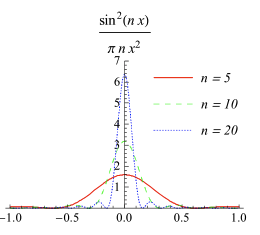
\includegraphics[width=0.9\textwidth,height=2.3in]{figs/5-1.png}
				  \end{center}
			\end{column}
		\end{columns}
\end{frame}

\begin{frame}
	\frametitle{}
	\例 [7. 试证明$\delta$函数的微分公式 ]
	{\[ \delta(x)=\frac{dH(x)}{dx}, \qquad H(x)
		=\left\{\begin{array}{c}
			0, \qquad(x<0) \\
			1, \quad(x >= 0)
			\end{array}\right. \]}
	\证 \[
		\begin{aligned}
		  \int_{-\infty}^{+\infty} \frac{dH(x)}{dx} \psi (x) d x &= H(x) \psi (x)\mid_{-\infty}^{+\infty} - \int_{-\infty}^{+\infty} H(x) \psi' (x) d x \\
		    &=  \psi (+\infty) - \int_{0}^{+\infty} \psi' (x) d x\\
			&=  \psi (+\infty)- \psi (+\infty)+\psi (0)\\
			&=  \psi (0) \\ 
			&=\int_{-\infty}^{+\infty} \delta(x) \psi (x) d x
		\end{aligned}
		   \]
		证毕!
\end{frame}

\begin{frame}
	\frametitle{}
	\例 [8. 试证明$\delta$函数的展开公式]
	{}
	 \[
		\begin{aligned}
		  \delta (\vec{r}-\vec{r}_0) &=  \delta (x-x_0) \delta (y-y_0) \delta (z-z_0)\\
		  &=  \frac{1}{r}\delta (r-r_0) \delta (\theta -\theta_0) \\
		  &=  \frac{1}{r^2\sin\theta}\delta (r-r_0) \delta (\theta -\theta_0) \delta (\varphi -\varphi_0)
		\end{aligned}
		   \]
\end{frame}

%%%%%%%%%%%%%%%%%%%%%%%%%%%%%%%%%%%%%%%%%%%%%%%%%%%%%%%%%%%%%%%%%%%
\begin{frame}
	\frametitle{课堂作业}
	 \begin{exampleblock}{1. 试证明:}
	 \[
	\int_{-\infty}^{+\infty} 1 \cdot e^{2\pi i kx} d x = \delta(k)
	\]
	 \end{exampleblock}
	\begin{exampleblock} {2. 求动量表象波函数}
	{已知坐标表象的波函数如下,现基于$\delta$函数求动量表象的波函数 $c(p)$}
		\begin{equation*}
			\Psi(x)=\frac{1}{\sqrt{2\pi \hbar}}  \int_{-\infty}^{+\infty} c(p) e^{\frac{i}{\hbar} px} dp 
		\end{equation*}   	
	\end{exampleblock}
\begin{exampleblock} {3. 证明第一类贝塞尔函数的正交性公式}
	\[\int_{0}^{+\infty} J_n(kr)J_n(k'r) r dr = \frac{\delta(k-k')}{k}, \qquad (m\geq-1; k, k'>0)\]  	
	\end{exampleblock}
\end{frame}
%%%%%%%%%%%%%%%%%%%%%%%%%%%%%%%%%%%%%%%%%%%%%%%%%%%%%%%%%%%%%%%%%%%                        %
%-----------------------------------------------%


\begin{frame}[plain]
    \Background[16] 
	\begin{center}
		{\huge \color{deepred} \textrm{Thanks for your attention!  \\ \vspace{1.0em}
         A \& Q}}
	\end{center}
    \addtocounter{framenumber}{-1} 
\end{frame}

%%%%%%%%%%%%%%%%%%%%%%%%%%%%%%%%%%%%%%%%%
\end{document}
%---------------THE END-----------------%


